\documentclass[11pt,oneside]{book}
\usepackage{fontspec}
\setmainfont{Noto Serif}
\setsansfont{Noto Sans}
\setmonofont{Noto Sans Mono}
\newfontfamily\proseunicodefont{DejaVu Serif}
\usepackage[margin=1in]{geometry}
\usepackage{microtype}
\usepackage{amsmath,amssymb,amsthm,mathtools,bm}
\usepackage{graphicx}
\usepackage{xcolor}
\usepackage{booktabs}
\usepackage{array}
\usepackage{longtable}
\usepackage{enumitem}
\usepackage{float}
\usepackage{caption}
\usepackage{hyperref}
\usepackage{fancyhdr}
\usepackage{tikz}
\usetikzlibrary{arrows.meta,positioning,calc,decorations.pathmorphing}

\hypersetup{
  colorlinks=true,
  linkcolor=blue!50!black,
  urlcolor=blue!50!black,
  citecolor=blue!50!black
}

\setlength{\parskip}{0.5em}
\setlength{\parindent}{0pt}
\setlist[itemize]{topsep=0.25em,itemsep=0.2em}
\setlist[enumerate]{topsep=0.25em,itemsep=0.2em}
\setlength{\headheight}{40pt}
\numberwithin{equation}{chapter}

\newtheorem{theorem}{Теорема}[chapter]
\newtheorem{proposition}[theorem]{Утверждение}
\newtheorem{lemma}[theorem]{Лемма}
\newtheorem{corollary}[theorem]{Следствие}
\theoremstyle{definition}
\newtheorem{definition}[theorem]{Определение}
\newtheorem{example}[theorem]{Пример}
\theoremstyle{remark}
\newtheorem{remark}[theorem]{Замечание}

\providecommand{\ket}[1]{\left\lvert#1\right\rangle}
\providecommand{\bra}[1]{\left\langle#1\right\rvert}
\providecommand{\braket}[2]{\left\langle#1\,\middle|\,#2\right\rangle}
\providecommand{\expect}[1]{\left\langle#1\right\rangle}
\newcommand{\lectureoverview}[1]{\paragraph{Обзор.} #1}

\makeatletter
\newcommand{\course@headerfont}{\normalfont\small\itshape}
\newcommand{\course@pagefont}{\normalfont\small}
\newcommand{\course@headerraise}{14pt}
\newlength{\course@headerboxheight}
\setlength{\course@headerboxheight}{\dimexpr\headheight-\course@headerraise-9pt\relax}
\newcommand{\course@leftheadbox}[1]{%
  \raisebox{\course@headerraise}{%
    \parbox[t][\course@headerboxheight][t]{0.82\textwidth}{%
      \raggedright\course@headerfont\strut\MakeUppercase{#1}\strut%
    }%
  }%
}
\newcommand{\course@rightheadbox}[1]{%
  \raisebox{\course@headerraise}{%
    \parbox[t][\course@headerboxheight][t]{0.82\textwidth}{%
      \raggedleft\course@headerfont\strut\MakeUppercase{#1}\strut%
    }%
  }%
}
\renewcommand{\chaptermark}[1]{\markboth{\MakeUppercase{\chaptername\ \thechapter.\ #1}}{}}
\renewcommand{\sectionmark}[1]{\markright{\MakeUppercase{\thesection\hspace{0.4em}#1}}}
\fancyhf{}
\fancyhead[L]{\course@leftheadbox{\leftmark}}
\fancyhead[R]{\course@pagefont\thepage}
\renewcommand{\headrulewidth}{0.5pt}
\pagestyle{fancy}
\fancypagestyle{plain}{%
  \fancyhf{}
  \fancyhead[L]{\course@leftheadbox{\leftmark}}
  \fancyhead[R]{\course@pagefont\thepage}
  \renewcommand{\headrulewidth}{0.5pt}
}
\makeatother

% Reader-facing provenance for classroom exchanges and editorial additions.
\newenvironment{classroomqa}{%
  \par\medskip\noindent\begin{minipage}{\linewidth}\small\hrule\medskip
}{%
  \medskip\hrule\end{minipage}\par\medskip
}
\newcommand{\audiencequestion}[1]{\noindent\textbf{Вопрос из аудитории.} #1\par\smallskip}
\newcommand{\lecturerresponse}[1]{\noindent\textbf{Ответ.} #1\par}
\newcommand{\lecturetimestamp}[1]{\footnote{Время в лекции: #1.}}
\newcommand{\lectureframe}[1]{\par\smallskip{\centering\footnotesize\itshape Кадр лекции: #1.\par}}
\newcommand{\editorialnote}[1]{\footnote{Редакторское пояснение: #1}}

\usepackage{polyglossia}
\setdefaultlanguage{russian}
\usepackage{sectsty}
\renewcommand{\contentsname}{Содержание}
\renewcommand{\chaptername}{Глава}
\renewcommand{\figurename}{Рисунок}
\renewcommand{\tablename}{Таблица}
\renewcommand{\proofname}{Доказательство}
\renewcommand{\bibname}{Литература}
\sectionfont{\raggedright}
\subsectionfont{\raggedright}
\makeatletter
\renewcommand{\@pnumwidth}{2.2em}
\renewcommand{\@tocrmarg}{3.2em}
\makeatother
\usepackage{tocloft}
\renewcommand{\cftchapfont}{\small\bfseries}
\renewcommand{\cftchappagefont}{\small\bfseries}
\renewcommand{\cftsecfont}{\small}
\renewcommand{\cftsecpagefont}{\small}
\setlength{\cftsecnumwidth}{3em}
\renewcommand{\cftsubsecfont}{\small}
\renewcommand{\cftsubsecpagefont}{\small}
\setlength{\cftsubsecindent}{4.5em}
\setlength{\cftsubsecnumwidth}{4em}
\emergencystretch=6em
\pdfstringdefDisableCommands{\def\proseunicodefont{}}

\geometry{paperwidth=177.6mm,paperheight=252mm,left=16mm,right=16mm,
 top=18mm,bottom=18mm,includeheadfoot,headheight=28pt,headsep=7mm,footskip=9mm}
\usepackage{scrextend}
\changefontsizes[17pt]{12pt}
\raggedbottom
\renewenvironment{classroomqa}{\par\medskip\begingroup}{\par\endgroup\medskip}
\fancyhf{}
\setlength{\headwidth}{\textwidth}
\fancyhead[L]{\parbox{\textwidth}{\raggedright\fontsize{9}{11}\selectfont\nouppercase{\leftmark}}}
\fancyfoot[C]{\small\thepage}
\renewcommand{\headrulewidth}{0.3pt}
\fancypagestyle{plain}{\fancyhf{}\fancyfoot[C]{\small\thepage}\renewcommand{\headrulewidth}{0pt}}

\hypersetup{
  pdftitle={Topics in String Theory},
  pdfauthor={Leonard Susskind},
  pdfsubject={Independently edited companion notes for the 2011 Winter lecture course},
  pdfcreator={LaTeX with hyperref}
}
\graphicspath{{../../../generated_course_notes/supplementary/cosmology_and_black_holes/2011_winter_topics_in_string_theory/figures/}{../../../generated_course_notes/supplementary/cosmology_and_black_holes/2011_winter_topics_in_string_theory/assets/}}
\begin{document}
\frontmatter
\hypersetup{pageanchor=false}
\begin{titlepage}
\hyphenpenalty=10000\exhyphenpenalty=10000
\thispagestyle{empty}
\begin{tikzpicture}[remember picture,overlay]
  \node[anchor=center,inner sep=0] at (current page.center) {%
    \includegraphics[height=\paperheight,keepaspectratio]{../../../generated_course_notes/supplementary/cosmology_and_black_holes/2011_winter_topics_in_string_theory/assets/cover-art.png}%
  };
  \node[
    anchor=north west,
    align=left,
    text width=0.78\paperwidth,
    fill=white,
    fill opacity=0.9,
    rounded corners=8pt,
    inner xsep=10pt,
    inner ysep=8pt
  ] at ([xshift=0.08\paperwidth,yshift=-0.06\paperheight]current page.north west) {%
    {\fontsize{30}{33}\selectfont\bfseries\color{black!88} Темы теории струн\\[0.85em]}
    {\large\color{black!72} Русское издание / зима 2011, темы по теории струн}
  };
  \node[
    anchor=south west,
    align=left,
    text width=0.68\paperwidth,
    fill=white,
    fill opacity=0.82,
    text opacity=1,
    rounded corners=6pt,
    inner sep=12pt
  ] at ([xshift=0.08\paperwidth,yshift=0.08\paperheight]current page.south west) {%
    {\normalsize\color{black!78} Оригинальные лекции: Leonard Susskind\\[0.35em]}
    {\small\color{black!72} Сопроводительное издание: \href{https://lazying.art}{LazyingArt LLC} / \href{https://github.com/lachlanchen/Video2Book}{Video2Book}}
  };
\end{tikzpicture}
\mbox{}
\end{titlepage}
\hypersetup{pageanchor=true}

\clearpage
\chapter*{Об этих конспектах}
Эти независимо отредактированные сопроводительные конспекты основаны на лекциях Леонарда Сасскинда. Они были восстановлены по машинным расшифровкам, субтитрам и отобранным кадрам с изображением доски, а затем сверены с доступными исходными материалами. Они не являются оригинальной рукописью профессора Сасскинда и не были им просмотрены или одобрены.

Издание подготовлено \href{https://lazying.art}{LazyingArt LLC} с использованием инструментария \href{https://github.com/lachlanchen/Video2Book}{Video2Book} с открытым исходным кодом. Машинные расшифровки по-прежнему доступны отдельно и могут содержать ошибки распознавания. Редакторские уточнения и нетривиальные реконструкции отмечены в сносках.
\clearpage
\tableofcontents
\mainmatter
\chapter{Лекция 1: Темы теории струн}

\lectureoverview{Вызов редукционизму становится острее благодаря бозонизации в \(1+1\) измерениях, электрической--магнитной дуальности, D-бранам, переходам при сильной связи, эмерджентной геометрии и комбинаторному ландшафту струнных вакуумов. Одна и та же физическая система может допускать радикально разные элементарные описания; то, какое из них выглядит простым, зависит от константы связи и геометрии.}

\section{Редукционизм, сложность и вопрос о простоте}

Сасскинд начинает с намеренно знакомого философского лозунга: большие вещи состоят из маленьких, а маленькие — из еще меньших. Затем он добавляет более амбициозную версию той же идеи, ту, которая действительно важна для фундаментальной физики: по мере спуска к более глубоким слоям объекты должны становиться не только меньше, но и проще. Его метафора такова: дома сделаны из кирпичей, и никто не примет дом за кирпич. Кирпич меньше, но он и проще.

Первый шаг лекции — сопоставить это ожидание с реальным состоянием физики частиц. Если бы редукционизм действительно приносил возрастающую простоту в этом сильном смысле, можно было бы ожидать, что современная физика элементарных частиц уже будет устроена экономно. Вместо этого Сасскинд подчеркивает, что еще до включения квантовой гравитации учет уже выглядит громоздким. В лекции приводятся грубые подсчеты, но эта грубость и есть часть замысла:
\begin{equation}
\begin{aligned}
N_{\mathrm{species}}&\sim 75,\\
N_{\mathrm{independent}}&\sim 10\text{--}20,\\
N_{\mathrm{parameters}}&\sim 20.
\end{aligned}
\end{equation}
Но и этим история не заканчивается. Стандартная модель не содержит гравитации, не объясняет темную материю, не дает дополнительной структуры, необходимой для инфляции, и несет в себе серьезную проблему тонкой настройки. Добавление обычных механизмов исправления лишь увеличивает число параметров. Примером в лекции служит суперсимметрия. Во время этой лекции многие физики надеялись, что Большой адронный коллайдер обнаружит суперпартнеров; Сасскинд подчеркивает, что соответствующее расширение ввело бы более ста дополнительных параметров, а не сразу упростило бы эту схему учета. Схематически его мысль такова
\begin{equation}
N_{\mathrm{parameters}}^{\mathrm{extended}} \sim 200.
\end{equation}
Эти числа намеренно грубы и имеют исторический характер. Они служат аргументом в пользу того, что более глубокое описание не обязано выглядеть проще на уровне перечня частиц и измеряемых констант.

Это количественное возражение — еще не главный тезис Сасскинда. Это лишь прелюдия. Более глубокое утверждение, и именно оно ведет дальнейшую часть лекции, состоит в том, что современная квантовая теория поля и теория струн, вообще говоря, не дают очевидного основания для единственного, не зависящего от константы связи различия между кирпичами и домами. Следующие примеры выбраны так, чтобы показать, что сам смысл ``элементарного'' может зависеть от того, какие переменные оказываются эффективными.

\section{Бозонизация: первый подрыв идеи фиксированной фундаментальности}

Первый теоретический пример Сасскинда взят из квантовой теории поля в \(1+1\) измерениях: одно пространственное измерение и одно временное. Он сразу оговаривает, что не будет подробно выводить эту эквивалентность; смысл не в формальном доказательстве, а в концептуальном уроке.

Начинают с теории поля фермионов. Фермионное поле обозначается \(\psi\). Два близко расположенных фермиона могут образовать бозонный композит, и соответствующее бозонное поле обозначается \(\phi\). На первый взгляд иерархия кажется ясной: \(\psi\) первично, тогда как \(\phi\) — составная или эффективная переменная. В лекции бозон вводится именно так, как поле, создающее связанные пары фермионов.

Однако было обнаружено, что ту же теорию можно переписать, исходя из противоположной отправной точки. Можно начать с бозонного поля \(\phi\), и тогда фермион больше не возникает как точечный компонент. Вместо этого он появляется как кинк бозонного поля — протяженная конфигурация, в которой \(\phi\) гладко интерполирует между двумя асимптотическими значениями. Минимальное математическое содержание лекции состоит в следующей асимптотической структуре:
\begin{equation}
\phi(x\to -\infty)=\phi_-,
\qquad
\phi(x\to +\infty)=\phi_+.
\end{equation}
Удобный схематический представитель имеет вид
\begin{equation}
\phi(x)\approx \frac{\phi_++\phi_-}{2}
+
\frac{\phi_+-\phi_-}{2}\tanh\!\left(\frac{x}{\ell}\right),
\end{equation}
где \(\ell\) — ширина переходной области.

\editorialnote{Профиль с гиперболическим тангенсом — стандартный гладкий представитель кинка, изображенного в лекции, а не формула, выведенная в ней. Точный словарь бозонизации зависит от модели; концептуально важно здесь то, что фермионное возбуждение и топологический солитон бозонного поля меняются ролями.}

Аналогия с ремнем в лекции достаточно точна, чтобы ее стоило сохранить. Плоский ремень без перекрута — это конфигурация без кинка. Если повернуть один конец на \(2\pi\), вдали ремень возвращается к той же локальной ориентации, но между этими областями он должен пройти через протяженную перекрученную область. Эта перекрученная область и есть кинк. В бозонном описании фермион представлен именно таким протяженным объектом.

Эта мысль становится резче, как только вводится константа связи. В этом примере Сасскинд обозначает ее \(G\). Утверждается не то, что эти два описания как-то расплывчато связаны, а то, что их эффективность зависит от режима параметров:
\begin{align}
G \ll 1
&\Rightarrow
\ell\text{ small, tight kink; }\psi\text{ efficient},\\
G \gg 1
&\Rightarrow
\ell\text{ large, broad kink; }\phi\text{ efficient}.
\end{align}
При малом \(G\) кинк компактен, и именно фермион выглядит простым объектом. По мере роста \(G\) кинк расширяется, и фермион становится менее точечноподобным. Тогда более экономичными оказываются бозонные переменные.

\paragraph{Схематическое правило перехода.}
\begin{enumerate}
\item Начните с фермионной теории, описываемой \(\psi\).
\item Выделите бозонные композиты, описываемые \(\phi\).
\item Перепишите ту же теорию целиком через \(\phi\).
\item В бозонном описании фермион снова возникает как кинк ширины \(\ell\).
\item При \(G\ll 1\) \(\ell\) мало, и самым простым оказывается фермионное описание.
\item При больших \(G\) \(\ell\) растет, и самым простым становится бозонное описание.
\end{enumerate}

Это первый явный контрпример к фиксированной картине ``домов и кирпичей''. Главная мысль лекции не просто в том, что существуют составные объекты, а в том, что то, что считается элементарной переменной, может меняться при изменении константы связи.

\section{Электрический заряд, магнитные монополи и режимы слабой и сильной связи}

Затем Сасскинд спрашивает, возникает ли аналогичная история в более привычной физике частиц. Примером служит электрический заряд в сравнении с магнитным монополем. Обычная заряженная частица, например электрон, в этой терминологии является электрическим монополем: локализованным источником электрического поля. Магнитный монополь вводится через аналогию со стержневым магнитом. Если бы удалось каким-то образом изолировать конец стержневого магнита без невидимого соединительного стержня, силовые линии выглядели бы в точности как у электрического заряда, только магнитные, а не электрические.

Существенным управляющим параметром является постоянная тонкой структуры \(\alpha\). В лекции Сасскинд эвристически трактует ее как квадрат электрического заряда:
\begin{equation}
\alpha \sim e^2.
\end{equation}
Он также дает грубое операционное толкование: она измеряет, насколько легко электрон излучает, и суммирует эту силу, говоря, что ускоренный электрон в соответствующем смысле излучает порядка ``\(1/100\)'' фотонов. В грубом численном языке самой лекции,
\begin{equation}
\alpha \approx 10^{-2}.
\end{equation}
Это не следует понимать как точную конвенцию; это педагогический способ выразить, что электрический заряд слаб.

\editorialnote{Связь слабой--сильной связи имеет точный прообраз в квантовании Дирака. В одном распространенном соглашении электрический и магнитный заряды удовлетворяют \(e g_m=2\pi n\). Следовательно, слабой электрической связи соответствует сильная магнитная, хотя точные численные множители и защищенные соотношения для масс зависят от теории.}

Когда \(\alpha\ll 1\), электрон является простым объектом. Его электрическое поле слабо, облако поляризации вакуума разрежено, и он выглядит почти точечным. Магнитный монополь тогда противоположен ему: его поле огромно, его окрестность резко искажена, и сам он протяжен, сложен и тяжел. Сасскинд резюмирует ситуацию именно в этом стиле слабой--сильной связи:
\begin{equation}
\begin{aligned}
\alpha \ll 1
&\Rightarrow \text{simple electron;}\\
&\phantom{\Rightarrow{}}\text{heavy, extended monopole},\\
\alpha \gg 1
&\Rightarrow \text{simple monopole;}\\
&\phantom{\Rightarrow{}}\text{heavy, structured electron}.
\end{aligned}
\end{equation}
В лекции не выводится формула массы монополя. В ней нет необходимости. Суть здесь качественная. По мере увеличения \(\alpha\) поле электрона усиливается и его структура разрастается, тогда как монополь сжимается и становится легче. При значениях, намного превышающих единицу, удобное описание меняется местами: прост монополь, а электрон сложен.

Это полевотеоретическая версия прежнего урока бозонизации. Различие между фундаментальным и составным не является абсолютным. Оно зависит от константы связи.

\begin{classroomqa}
\audiencequestion{Если редукционизм не является надёжным ориентиром, почему физики полагаются на математический анализ, который, по-видимому, делит систему на сколь угодно малые части? \lecturetimestamp{00:21:21}}
\lecturerresponse{Математический анализ утверждает гладкое изменение; он не определяет фундаментальные объекты теории. Квантовые поля флуктуируют на всех масштабах расстояния, порождая бесконечную иерархию, а не некоторый последний гладкий слой, на котором можно было бы раз и навсегда решить, что является элементарным.}
\end{classroomqa}

Обмен репликами продолжается предположением, что эта иерархия напоминает фрактал. Сасскинд принимает аналогию, а затем уточняет её: квантовые поля флуктуируют на всех масштабах и потому никогда не являются гладкими в классическом смысле. Эта чрезмерная изменчивость — часть того, что делает квантовую теорию поля математически трудной; обычный математический анализ приходится применять к перенормированным величинам, а не к наивно гладкому микроскопическому полю.

\section{Струны, D-браны и возвращение слабой--сильной дуальности}

Следующий переход в лекции намеренно наивен. Если теория струн должна быть теорией фундаментальных составляющих, то ответ, конечно, должен быть прост: этими составляющими являются струны. Сасскинд открыто формулирует это ожидание, а затем посвящает следующую часть лекции тому, чтобы его разобрать.

\subsection{Почему струны — не вся история}

Первая трудность состоит в неизбежном присутствии D-бран. D\(p\)-брана — это \(p\)-мерный объект, на котором могут оканчиваться струны. Буква \(D\) происходит от граничных условий Дирихле, но имя гораздо менее важно, чем роль: эти объекты входят в теорию и не могут быть отброшены. Это не факультативные украшения.

Простейшие примеры таковы:
\begin{itemize}
\item D0-брана, которая является точечным объектом,
\item D1-брана, или D-струна, которая является струноподобным объектом,
\item F-струна, обычная фундаментальная струна.
\end{itemize}
D0-брана — это тяжёлый точечный узел, на котором может оканчиваться сколь угодно много F-струн. D1-брана — тяжёлый кабелеобразный объект, гораздо более толстый и обладающий гораздо большей массой на единицу длины, чем F-струна, но также служащий местом, где могут оканчиваться F-струны. При слабой связи лекция не представляет эти объекты как в равной мере элементарные альтернативы. D-браны вводятся как тяжёлые, структурированные, на вид составные объекты, которые теория, тем не менее, навязывает нам.

\editorialnote{Используемая в этой части лекции теория с нечётными бранами — это теория струн типа IIB. Её стабильные D-браны имеют нечётную пространственную размерность, включая D1- и D3-браны. Сасскинд откладывает эти названия, поскольку непосредственная тема — схема дуальности, а не таксономия.}

\paragraph{Обозначения.}
Сасскинд несколько вольно использует \(G\) и \(g\) в разных частях лекции. Здесь \(G\) зарезервировано для примера с бозонизацией, тогда как \(g\) обозначает струнную константу связи.

Струнная константа связи \(g\) определяется операционально, а не аксиоматически. Это параметр, измеряющий вероятность того, что флуктуирующая струна расщепится и образует дочерние струны. Поэтому Сасскинд напрямую сравнивает её с ролью \(\alpha\) в КЭД. В лекции также делается пауза, чтобы отождествить натяжение с энергией на единицу длины:
\begin{equation}
T=\frac{E}{L}=\frac{M}{L}.
\end{equation}

Для F-струны и D-струны стандартные формулы для натяжения делают сравнение слабой--сильной связи явным:
\begin{equation}
T_{\mathrm{F1}}=\frac{1}{2\pi\alpha'},
\qquad
T_{\mathrm{D1}}=\frac{1}{2\pi\alpha' g_s},
\qquad
\frac{T_{\mathrm{D1}}}{T_{\mathrm{F1}}}=\frac{1}{g_s}.
\end{equation}
\editorialnote{Эти формулы для натяжения задают общепринятую нормировку, стоящую за качественным сопоставлением кабеля и нити в лекции. Это редакторское добавление; в самой лекции используется только зависимость от константы связи.}

\subsection{F-струны и D-струны}

Затем история слабой--сильной связи повторяется на языке струн. При малой связи F-струна легка, тонка и близка к исходному интуитивному образу фундаментального объекта. D-струна толста, тяжела и наполнена структурой из F-струн. По мере роста связи F-струна легче расщепляется; облако дочерних струн вокруг неё разрастается, и она становится тяжелее и сложнее. В то же время D-струне всё труднее испускать ставшие теперь тяжёлыми F-струны, так что окружающая её структура редеет, и она становится легче и более нитевидной. Поэтому схема слабой--сильной связи в лекции такова
\begin{align}
g \ll 1
&\Rightarrow
\begin{gathered}
\text{F-string light and thin;}\\
\text{D-string heavy and structured},
\end{gathered}\\
g \sim 1
&\Rightarrow
\text{F-string and D-string comparable},\\
g \gg 1
&\Rightarrow
\begin{gathered}
\text{D-string light and thin;}\\
\text{F-string heavy and structured}.
\end{gathered}
\end{align}
Сасскинд замечает, что вблизи \(g\sim 1\) эти два описания перестают чётко различаться. За этой точкой они фактически меняются ролями. Это струнно-теоретическая версия обмена электрон--монополь, и её общепринятое название — S-дуальность.

Тот же обмен можно проследить и после того, как струна замыкается в петлю. При слабой связи маленькая петля F-струны является лёгким частицеподобным возбуждением, тогда как соответствующая петля D-струны тяжела и сложна. При сильной связи их роли меняются: петля D-струны становится лёгким описанием, и среди возникающих при этом лёгких возбуждений замкнутой струны есть гравитон. Этот пример в лекции нужен для того, чтобы настоять: даже тождество знакомой частицы может зависеть от того, с какой стороны дуальности ведётся описание.

Лекция продвигает эту мысль ещё на один шаг. В идеализированной теории константа связи — не просто число, которое можно выставлять вручную; она ведёт себя как поле. Схематически,
\begin{equation}
g = g(x).
\end{equation}
Поэтому в разных областях пространства могут быть предпочтительны разные дуальные описания. В одной области лёгкими переменными являются F-струны; в другой — D-струны. Между ними ничто не является особенно простым. Вот почему, с точки зрения Сасскинда, теория струн не восстанавливает простую редукционистскую картину. Она радикализует эту неоднозначность.

\editorialnote{В пертурбативной теории струн локальная константа связи задаётся дилатоном, \(g_s(x)=e^{\Phi(x)}\). Поэтому запись \(g=g(x)\) — не просто аналогия, хотя реалистические компактификации, как правило, порождают потенциал, который ограничивает такие вариации.}

\begin{classroomqa}
\audiencequestion{Если бы константа связи менялась настолько, что в другой области D-струны становились бы легче F-струн, повлияло бы это изменение на наблюдаемые спектры? \lecturetimestamp{00:34:15}}
\lecturerresponse{Да. Это одна из причин, по которым обсуждаемую точно симметричную, математически контролируемую модель нельзя напрямую отождествить с нашим миром. Её уроки касаются того, на что способны непротиворечивые квантовые теории, а не буквального спектра природы.}
\end{classroomqa}

\begin{classroomqa}
\audiencequestion{Существует ли аналогичное дуальное описание для D2-браны? \lecturetimestamp{00:34:39}}
\lecturerresponse{Да, но это не ещё один обмен по типу D-струны. Случай чётных бран приведёт к мембранной интерпретации и к дополнительному пространственному измерению; это и есть следующая конструкция.}
\end{classroomqa}

\begin{classroomqa}
\audiencequestion{Объясняет ли большая вероятность расщепления струны возросшую внутреннюю сложность? \lecturetimestamp{00:34:53}}
\lecturerresponse{Да. Чтобы сделать механизм наглядным, вернёмся к КЭД: электрон испускает фотоны, фотоны флуктуируют в заряженные пары, а эти заряженные линии снова излучают. При увеличении связи эта иерархия становится менее разреженной.}
\end{classroomqa}

\subsection{Возвращение к квантовой электродинамике в ответ на вопросы}

Затем студент спрашивает, означает ли большая вероятность расщепления просто более сложную структуру ``выше по иерархии''. Сасскинд отвечает, возвращаясь к квантовой электродинамике и снова рисуя мировую линию электрона. Это возвращение важно: оно показывает, что история со струнами — не изолированная диковина, а ещё один случай той же схемы слабой--сильной связи.

\begin{figure}[htbp]
\centering
\begin{tikzpicture}[scale=1.0]
\draw[->] (-1.2,0) -- (3.7,0) node[right] {space};
\draw[->] (0,-0.2) -- (0,4.3) node[above] {time};

\draw[line width=0.9pt] (0,0.2) -- (0,4.0);
\node[left] at (0,3.55) {\(e^{-}\)};

\draw[line width=0.8pt] (0,1.0) -- (0.18,1.08) -- (0.36,0.92) -- (0.54,1.10) -- (0.72,0.94) -- (0.90,1.12) -- (1.08,0.96) -- (1.26,1.14);
\draw[line width=0.8pt] (0,2.35) -- (-0.18,2.43) -- (-0.36,2.27) -- (-0.54,2.45) -- (-0.72,2.29) -- (-0.90,2.47);

\draw[line width=0.8pt] (1.26,1.14) -- (1.48,1.42);
\draw[line width=0.8pt] (1.26,1.14) -- (1.04,1.42);
\draw[line width=0.8pt] (1.48,1.42) -- (1.58,2.10);
\draw[line width=0.8pt] (1.04,1.42) -- (0.94,2.10);
\draw[line width=0.8pt] (0.94,2.10) -- (1.58,2.10);

\draw[line width=0.7pt] (1.58,1.78) -- (1.72,1.84) -- (1.86,1.72) -- (2.00,1.86);
\draw[line width=0.7pt] (0.94,1.78) -- (0.80,1.84) -- (0.66,1.72) -- (0.52,1.86);

\node at (2.35,1.95) {\(\gamma\)};
\node at (-1.15,2.75) {\(\gamma\)};
\end{tikzpicture}
\caption{Схематическая иерархия КЭД, используемая в лекции: точечный электрон испускает фотоны, фотоны создают пары, а дочерние заряженные линии снова излучают, порождая структуру на всё меньших масштабах.}
\end{figure}

Идея лекции состоит в том, что даже точечный электрон сопровождается иерархией процессов:
\begin{enumerate}
\item электрон испускает и поглощает фотоны,
\item фотон может создать электрон--позитронную пару,
\item дочерние заряженные линии сами могут испускать фотоны,
\item иерархия продолжается к меньшим масштабам.
\end{enumerate}
При слабой связи это облако разрежено, поэтому в лаборатории электрон выглядит почти точечным. При более сильной связи оно разрастается, и электрон становится структурированным объектом. После этого история со струнами подаётся как прямой аналог этого.

Та же последующая дискуссия также служит мотивировкой для эвристического учёта энергии у Сасскинда. Он настаивает, что существенная энергия — не просто сумма вкладов свободных частиц. Нужно также учитывать энергию взаимодействия:
\begin{equation}
E_{\mathrm{tot}} = E_e + E_\gamma + E_{\mathrm{int}}.
\end{equation}
Здесь \(E_{\mathrm{int}}\) — ключевой член. Именно он позволяет массе одетого электрона включать энергию, связанную с окружающим его полем и виртуальной структурой. Лекция не превращает это в формальный вывод перенормированной собственной энергии. Тезис эвристичен, но существенен: масса объекта уже включает энергию взаимодействия, необходимую для поддержания сложного облака вокруг него.

\begin{classroomqa}
\audiencequestion{Откуда берётся энергия для виртуальных фотонов и электрон--позитронных пар, если электрон не содержит достаточно свободной энергии, чтобы создать реальную пару? \lecturetimestamp{00:37:01}}
\lecturerresponse{Никогда не начинают с голого электрона, а потом не присоединяют к нему его кулоновское поле. Наблюдаемый электрон — это одетое состояние, и его масса уже включает энергию поля и взаимодействия. В КЭД полная энергия — это не просто энергия свободного электрона плюс энергия свободного фотона; член взаимодействия незаменим. Называть промежуточные пары виртуальными полезно, но энергетический баланс относится к полному взаимодействующему состоянию.}
\end{classroomqa}

\begin{classroomqa}
\audiencequestion{Когда высокоэнергетический зонд выявляет эту структуру, не создаёт ли её сам зонд, вместо того чтобы обнаруживать нечто уже существующее? \lecturetimestamp{00:38:59}}
\lecturerresponse{Об этом различии в интерпретации можно спорить. В операционном смысле достаточно энергичное рассеяние имеет вычислимое нетривиальное конечное состояние. При слабой связи большинство событий по-прежнему выглядит простым, тогда как примерно в доле случаев порядка \(\alpha\) проявляются дополнительное излучение или пары.}
\end{classroomqa}

\begin{classroomqa}
\audiencequestion{Когда говорят, что D1-брана массивнее F-струны, означает ли это, что её натяжение тоже больше? \lecturetimestamp{00:39:37}}
\lecturerresponse{Да. Для протяжённой струны ``масса'' здесь означает энергию на единицу длины, что и есть в точности натяжение.}
\end{classroomqa}

\begin{figure}[htbp]
\centering
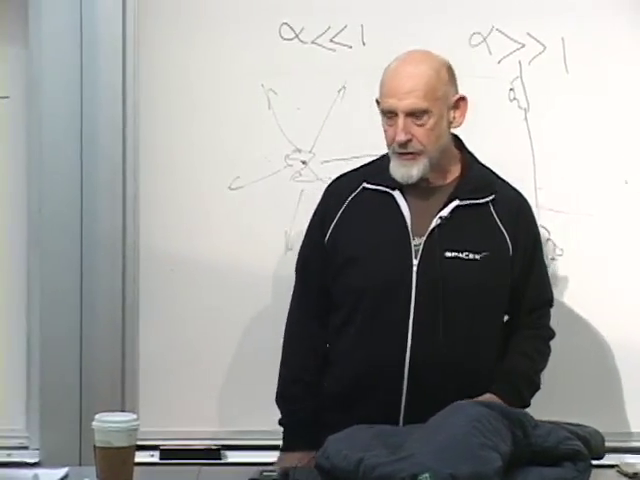
\includegraphics[width=0.72\textwidth]{lecture_01_figure_02.png}
\lectureframe{00:38:22.500}

\vspace{1em}

\begin{tikzpicture}[scale=0.95]
\draw (-5.3,-2.4) rectangle (-1.0,2.1);
\draw (0.3,-2.4) rectangle (4.6,2.1);

\node at (-3.15,2.55) {$\alpha \ll 1$};
\node at (2.45,2.55) {$\alpha \gg 1$};

\draw[line width=0.9pt] (-3.15,-0.15) circle (0.22);
\draw[->,line width=0.8pt] (-3.15,0.07) -- (-3.15,1.35);
\draw[->,line width=0.8pt] (-2.98,-0.01) -- (-1.95,1.00);
\draw[->,line width=0.8pt] (-3.32,-0.01) -- (-4.35,1.00);
\draw[->,line width=0.8pt] (-2.95,-0.23) -- (-1.80,-0.95);
\draw[->,line width=0.8pt] (-3.35,-0.23) -- (-4.50,-0.95);

\draw[line width=1.0pt] (2.15,-1.8) .. controls (1.95,-0.6) and (1.95,0.8) .. (2.15,1.55);
\draw[line width=1.0pt] (2.75,-1.8) .. controls (2.95,-0.6) and (2.95,0.8) .. (2.75,1.55);
\draw[line width=0.8pt] (2.15,-0.85) -- (2.75,-0.85);
\draw[line width=0.8pt] (2.45,1.55) -- (2.45,1.95);
\end{tikzpicture}
\caption{Сравнение слабой--сильной связи в КЭД в ходе обсуждения энергии взаимодействия. Диаграмма выделяет два режима, различимые в изложении Susskind: разрежённое облако при слабой связи и разрастающееся — при сильной.}
\end{figure}

Причина, по которой этот рисунок помещён именно здесь, хотя сравнение слабой--сильной связи было введено раньше, состоит в том, что в лекции Susskind заново проводит это противопоставление в этой более поздней, вызванной вопросом части, обсуждая энергию взаимодействия и разрастающуюся структуру.

\section{Теории с чётномерными бранами и возникающее дополнительное измерение}

До этого момента лекция выстраивала убедительный сюжет о взаимной замене: фермион против бозона, электрон против монополя, F-струна против D-струны. Следующий шаг ещё более удивителен. Susskind переходит к другой версии теории струн, с чётномерными D-бранами, а не с нечётномерными. Это различие существенно, потому что в этой теории нет D-струны, которую можно было бы обменять на F-струну. Здесь имеются D0-браны, D2-браны, D4-браны и так далее.

Поэтому предел сильной связи не может быть просто переименованием одной струны в другую. Согласно лекции, происходит нечто более странное: проявляется дополнительное пространственное измерение. Susskind намеренно сначала формулирует это в максимально драматической форме --- ``материализуется новое измерение'' ---, а затем сразу переводит это в более аккуратное утверждение: очень малое компактное направление расширяется, пока его уже нельзя игнорировать.

Этот учёт — часть самой идеи, поэтому он делает на нём паузу:
\begin{equation}
\begin{aligned}
10\text{-dimensional string theory} &= 9\text{ space}+1\text{ time},\\
11\text{-dimensional theory} &= 10\text{ space}+1\text{ time}.
\end{aligned}
\end{equation}
Согласно лекции, предел сильной связи теории с чётномерными бранами эффективно одиннадцатимерен.

\editorialnote{Теория с чётномерными бранами — это теория струн типа IIA, а её завершение при сильной связи — M-теория. В стандартных единицах радиус возникающей окружности и одиннадцатимерная планковская длина масштабируются как \(R_{11}=g_s\ell_s\) и \(\ell_{11}=g_s^{1/3}\ell_s\). Эти названия и формулы явно показывают современный словарь, стоящий за геометрическим изложением лекции.}

\subsection{Сэндвич с арахисовым маслом}

Чтобы наглядно представить компактное направление, Susskind использует модель ``сэндвича с арахисовым маслом'': две бесконечно тонкие ломтины хлеба, между которыми находится реальное пространство. Особое правило состоит в том, что выход через одну сторону возвращает на другую. В стандартном обозначении, которое в лекции описывается наглядно, а не формально, можно написать
\begin{equation}
y \sim y + 2\pi R.
\end{equation}
Если \(R\) очень мал, наблюдатели, живущие в этом сэндвиче, эффективно описывают свой мир как имеющий меньшую размерность. Тогда ключевое изменение при сильной связи таково:
\begin{equation}
g\uparrow
\qquad \Longrightarrow \qquad
R_{\mathrm{compact}}\uparrow.
\end{equation}
Вот что Susskind имеет в виду, когда говорит, что появляется новое измерение пространства: не то, что пространство создаётся из ничего, а то, что прежде крошечное компактное направление расширяется и становится видимым в эффективной теории.

\begin{figure}[htbp]
\centering
\resizebox{\linewidth}{!}{%
\begin{tikzpicture}[scale=0.95]
\draw[line width=0.9pt] (-5,1.7) -- (5,1.7);
\draw[line width=0.9pt] (-5,-1.7) -- (5,-1.7);

\node[left] at (-5,1.7) {ceiling};
\node[left] at (-5,-1.7) {floor};

\draw[->,line width=0.8pt] (5.2,1.45) -- (5.2,-1.45);
\draw[->,line width=0.8pt] (5.5,-1.45) -- (5.5,1.45);
\node[right] at (5.55,0) {periodic};

\draw[line width=1.0pt] (-2.6,0.45) -- (2.2,0.45);
\draw[line width=1.0pt] (-2.6,-0.05) -- (2.2,-0.05);
\draw[line width=1.0pt] (-2.6,0.45) -- (-2.6,-0.05);
\draw[line width=1.0pt] (2.2,0.45) -- (2.2,-0.05);
\node at (-0.2,0.9) {floating D2-brane};

\draw[line width=1.0pt] (3.15,-1.7) -- (3.8,-1.7);
\draw[line width=1.0pt] (3.15,1.7) -- (3.8,1.7);
\draw[line width=1.0pt] (3.15,-1.7) -- (3.15,1.7);
\draw[line width=1.0pt] (3.8,-1.7) -- (3.8,1.7);
\node[right] at (3.95,0) {D2 ribbon};

\fill (-3.8,0) circle (0.07);
\node[below] at (-3.8,-0.05) {D0};
\end{tikzpicture}
}%
\caption{Сэндвич-компактификация. Верхняя и нижняя границы периодически отождествляются; одна D2-брана парит между ними, как ковёр, а другая тянется от пола до потолка и выглядит струнообразной, когда компактное направление мало.}
\end{figure}

\subsection{Что происходит с D0- и D2-бранами?}

Теперь в лекции ставится вопрос о том, что происходит с D0-бранами и струнами. Ответ несимметричен. По мере роста \(g\) D0-браны делаются всё легче и легче; в более высокоразмерной интерпретации они входят в башню частиц, несущих импульс во вновь проявившемся направлении. Тем самым тяжёлый, сложный объект в картине слабой связи становится обычным лёгким возбуждением в картине сильной связи.

Соотношение масс показывает это отождествление:
\begin{equation}
M_{D0}(n)=\frac{n}{g_s\ell_s}
=\frac{n}{R_{11}}
=M_{\mathrm{KK}}(n).
\end{equation}
\editorialnote{Susskind называет D0-браны ``гравитонами'' одиннадцатимерной теории. Точнее, их связанные состояния — это моды импульса Калуцы--Клейна мультиплета одиннадцатимерной супергравитации, безмассовый сектор которого содержит гравитон. Это различие сохраняет физическое отождествление из лекции, избегая при этом слишком буквального утверждения на уровне одной частицы.}

D2-браны объясняют судьбу струн. В лекции выделены две конфигурации:
\begin{enumerate}
\item D2-брана, плавающая между полом и потолком, как ковёр в арахисовом масле;
\item D2-брана, натянутая от пола до потолка, как лента, и протянутая вдоль видимого направления.
\end{enumerate}
Когда сэндвич тонок, лента выглядит эффективно одномерной. Это тот объект, который наблюдатели низких энергий называют струной. По мере того как компактное направление раскрывается, тот же самый объект становится несомненно мембраноподобным. Поскольку теперь в вертикальном направлении в нём больше материала, он становится тяжёлым и уже не похожим на струну.

\paragraph{Логика перехода.}
\begin{enumerate}
\item Начните с очень тонкого компактного направления, так что лента от пола до потолка эффективно ведёт себя как струна.
\item С увеличением \(g\) компактное направление расширяется.
\item D0-браны становятся лёгкими и переинтерпретируются как состояния импульса Калуцы--Клейна в более высокоразмерной теории.
\item Струноподобная D2-лента становится явно протяжённой мембраной и тяжелеет.
\end{enumerate}
Это узловой переход лекции от дуальности к возникающей геометрии. Сильная связь не просто обменивает один объект на другой; она меняет то, какая геометрия является эффективной.

Susskind останавливается на том, насколько странно это звучит. Сеть предлагаемых отождествлений требовала трудных математических соотношений согласованности; некоторые из них сначала появились у физиков как гипотезы, а позднее были доказаны математиками. Он не утверждает, что каждый реалистический вакуум теории струн понят, но утверждает, что сама сеть дуальностей выдержала необычайно жёсткие проверки.

Если в этой идеализированной постановке константа связи меняется от места к месту, вместе с ней может меняться и эффективная геометрия. Одна область может выглядеть почти десятимерной, с лёгкими струнами и тяжёлыми D0-бранами; другая может раскрываться в одиннадцатимерное описание, с тяжёлыми обёрнутыми мембранами и лёгкими модами Калуцы--Клейна. Локальная смена языка описания — часть той же самой сети дуальностей.

Стенограмма кратко передаёт название этих соотношений как ``неравенства.'' По контексту имеется в виду слово \emph{дуальности}: связи между противоположными концами пространства параметров. Эта поправка важна, потому что вывод лекции как раз и состоит в том, что никакого единственного списка фундаментальных составляющих не известно. Струны, браны, частицы и геометрия более высоких измерений могут переходить друг в друга; либо ни один элемент этой сети не является абсолютно фундаментальным, либо какая-то более глубокая организация остаётся неизвестной.

\section{D3-браны, обёрнутые мембраны и геометрическая картина дуальности}

После перерыва Susskind прямо описывает эту тему как ``огромную сеть'' взаимосвязанных теорий и идей. Следующие примеры — это не новые изолированные эффекты; это мосты, связывающие предыдущие.

\subsection{Мировой объём D3-браны}

В первом мосте используется D3-брана. D3-брана имеет три пространственных измерения, и наблюдатель, ограниченный ею, легко может принять ее за обычное пространство. Брана может изгибаться и флуктуировать, а струны, оканчивающиеся на ней, могут соединяться, расщепляться и рассеиваться. Для наблюдателя, видящего только направления вдоль браны, каждый конец выглядит как частица, а взаимодействия между концами выглядят как обычная квантовая теория поля.

\begin{figure}[htbp]
\centering
\resizebox{\linewidth}{!}{%
\begin{tikzpicture}[scale=1.0]
\draw[fill=gray!15] (-4,-0.35) rectangle (4,0.35);
\node at (0,-0.75) {D3-brane};

\draw[line width=0.9pt] (-1.5,2.1) -- (-1.5,0.35);
\fill (-1.5,0.35) circle (0.07);
\node[left] at (-1.72,1.25) {F-string};
\node[below left] at (-1.5,0.32) {electric charge};

\draw[line width=1.5pt] (1.7,2.1) -- (1.7,0.35);
\fill (1.7,0.35) circle (0.09);
\node[right] at (1.95,1.25) {D-string};
\node[below right] at (1.7,0.32) {magnetic monopole};
\end{tikzpicture}
}%
\caption{Интерпретация на мировом объеме D3-браны. Конец F-струны выглядит как электрический заряд; конец D-струны — как магнитный монополь.}
\end{figure}

Это одно из самых удачных отождествлений в лекции. F-струна, оканчивающаяся на D3-бране, выглядит для наблюдателя на мировом объеме как электрический заряд. D-струна, оканчивающаяся на той же бране, выглядит как магнитный монополь. Иными словами, дуальность между F-струнами и D-струнами на мировом объеме D3-браны становится электрическо--магнитной дуальностью обычной теории поля. То, что раньше было аналогией, теперь стало явным словарем соответствий.

\editorialnote{Для стопки D3-бран низкоэнергетическое описание на мировом объеме представляет собой четырехмерную \(\mathcal N=4\) суперсимметричную теорию Янга--Миллса. Ее электрическо--магнитная дуальность является реализацией S-дуальности теории типа IIB на языке теории поля; одиночная брана дает абелев предел, использованный в лекции для наглядности.}

\subsection{Два компактных направления и асимметричное обертывание}

Затем Susskind возвращается к многомерной геометрии и компактифицирует не одно, а два малых направления. Поскольку изобразить на доске 11 измерений невозможно, он сжимает 7 больших направлений, не использованных в схеме, в одно видимое горизонтальное направление, а затем явно рисует два компактных. Он настаивает на асимметричном изображении компактификации, потому что одно компактное направление должно быть короче другого, если эффективные струны должны иметь разные натяжения.

\begin{figure}[htbp]
\centering
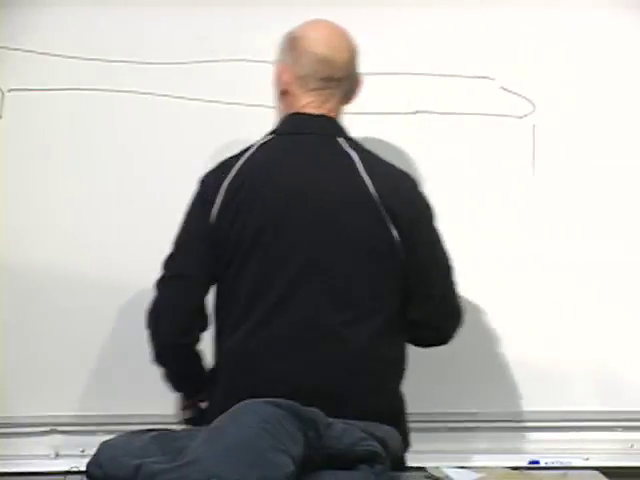
\includegraphics[width=0.78\textwidth]{lecture_01_figure_03.png}
\lectureframe{01:10:25.000}
\caption{Окончательный рисунок на доске для двух обернутых мембран. Короткий и длинный компактные циклы дают показанные справа ленты, подобные F- и D-струнам.}
\end{figure}

Мембрана может обертывать любое из компактных направлений и из некомпактных направлений выглядеть как струна. Если \(R_1\) и \(R_2\) — это два радиуса окружностей, то ее эффективные натяжения равны
\begin{equation}
\begin{aligned}
T_{(1)}&=2\pi R_1 T_{\mathrm{M2}},\\
T_{(2)}&=2\pi R_2 T_{\mathrm{M2}},\\
\frac{T_{(1)}}{T_{(2)}}&=\frac{R_1}{R_2}.
\end{aligned}
\end{equation}
Таким образом, неодинаковые размеры окружностей дают неодинаковые натяжения струн. Если отождествить более короткое обертывание с легкой F-струной, а более длинное — с тяжелой D-струной, то схематически можно написать
\begin{equation}
g_s\sim \frac{R_{\mathrm{short}}}{R_{\mathrm{long}}},
\qquad
\frac{T_{\mathrm{D1}}}{T_{\mathrm{F1}}}\sim \frac{1}{g_s}.
\end{equation}

\begin{classroomqa}
\audiencequestion{Можно ли в этой картине понимать константу связи как отношение двух компактных размеров? \lecturetimestamp{01:10:13}}
\lecturerresponse{Да. Параметр слабо--сильной связи геометризуется как отношение сторон. Если сделать одно направление коротким, константа связи станет малой; если поменять два направления местами, легкая и тяжелая струны поменяются ролями.}
\end{classroomqa}

\editorialnote{В лекции это отношение временно обозначается через \(\alpha\), то есть повторно используется символ, ранее употреблявшийся для постоянной тонкой структуры КЭД. Здесь мы пишем \(g_s\), чтобы различать эти два значения. В полном построении M-теории константа связи типа IIB кодируется комплексной структурой компактного двумерного тора; точный числитель зависит от того, как помечены его циклы.}

Картину с обернутыми мембранами можно подытожить без перспективных искажений рисунка на доске:

\begin{figure}[htbp]
\centering
\begin{tikzpicture}[scale=1.0]
\draw[line width=0.9pt] (0,0) rectangle (5.2,2.2);
\node[below] at (2.6,-0.2) {\(R_1\)};
\node[right] at (5.4,1.1) {\(R_2\)};

\draw[->,line width=0.7pt] (5.45,1.9) -- (5.45,0.3);
\draw[->,line width=0.7pt] (5.7,0.3) -- (5.7,1.9);
\draw[->,line width=0.7pt] (0.4,-0.35) -- (4.8,-0.35);
\draw[->,line width=0.7pt] (4.8,-0.6) -- (0.4,-0.6);

\draw[line width=1.0pt] (1.1,0) -- (1.6,0) -- (1.6,2.2) -- (1.1,2.2) -- cycle;
\node at (1.35,2.55) {light};

\draw[line width=1.0pt] (0,1.45) -- (5.2,1.45);
\draw[line width=1.0pt] (0,1.00) -- (5.2,1.00);
\node at (4.55,1.95) {heavy};

\node at (1.35,-0.95) {F-string};
\node at (4.55,0.55) {D-string};
\end{tikzpicture}
\caption{Обе конфигурации обернутой мембраны из некомпактных направлений выглядят как струны, но из-за неравных компактных масштабов одна эффективная струна оказывается легче другой.}
\end{figure}

Это геометрическая версия прежнего сюжета о дуальности. Сжатие одного направления при растяжении другого делает один обернутый объект тяжелее, а другой легче, так что роли F-струны и D-струны могут меняться местами.

\begin{classroomqa}
\audiencequestion{Если компактные направления циклические, не становятся ли обернутые объекты бесконечно широкими? \lecturetimestamp{01:10:41}}
\lecturerresponse{Нет. Компактная окружность имеет конечную длину, хотя по ней можно проходить снова и снова, не достигая края. Верх и низ разрезанного рисунка представляют одну и ту же точку, так же как концы интервала могут представлять одну точку окружности.}
\end{classroomqa}

\begin{figure}[htbp]
\centering
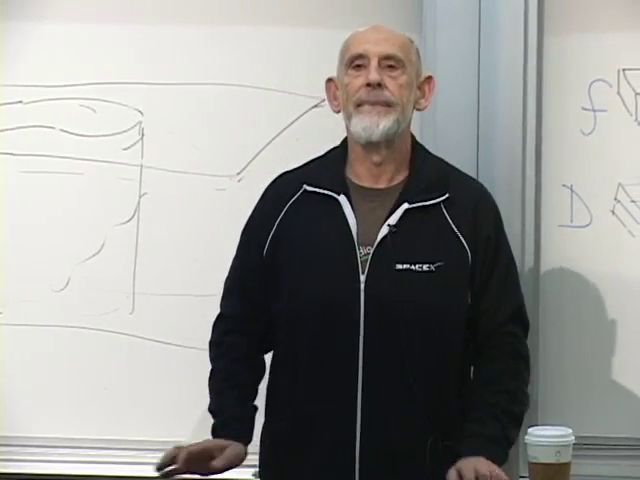
\includegraphics[width=0.78\textwidth]{lecture_01_figure_04.png}
\lectureframe{01:12:25.000}

\vspace{1em}

\begin{tikzpicture}[scale=0.95]
\draw[line width=0.9pt,->] (-3.7,0) arc[start angle=180,end angle=535,radius=0.95];
\node at (-2.75,0) {compact circle};
\draw[line width=0.9pt] (0.0,0) -- (4.8,0);
\fill (0.0,0) circle (0.06);
\fill (4.8,0) circle (0.06);
\draw[<->] (0.0,-0.45) -- (4.8,-0.45);
\node at (2.4,-0.75) {cut-open interval of length \(2\pi R\)};
\node[above] at (0.0,0.1) {same point};
\node[above] at (4.8,0.1) {same point};
\end{tikzpicture}
\caption{Компактная окружность и ее разрезанное изображение на доске. Переход через один конец возвращает к другому; движение по окружности при одновременном движении в некомпактном направлении дало бы вместо этого винтовую линию.}
\end{figure}

\begin{classroomqa}
\audiencequestion{Почему компактный путь — это окружность, а не винтовая линия? \lecturetimestamp{01:12:23}}
\lecturerresponse{В каждой фиксированной точке некомпактного направления компактное направление является окружностью. Винтовая линия появляется только тогда, когда движение по некомпактному направлению сопровождается одновременной намоткой вокруг окружности. Интервал на доске — это просто разрезанная окружность с отождествленными концами.}
\end{classroomqa}

\begin{classroomqa}
\audiencequestion{Объясняет ли сама эта геометрия, как D-брана при достаточно детальном зондировании может выглядеть как набор F-струн? \lecturetimestamp{01:12:49}}
\lecturerresponse{Связь здесь есть, но в этой элементарной картине она не прозрачна; чтобы ее увидеть, нужен более развитый геометрический аппарат. Диаграмма предназначена для организации дуальности, а не для вывода всякого описания на уровне микроскопических составляющих.}
\end{classroomqa}

\begin{classroomqa}
\audiencequestion{Могут ли длинное и короткое компактные направления меняться местами при перемещении в пространстве или по мере эволюции во времени? \lecturetimestamp{01:13:35}}
\lecturerresponse{В идеализированной модели возможно и то и другое. Если сжать один цикл и расширить другой, то меняется, какая из обернутых струн является легкой. Это еще одна причина, почему ``фундаментальная струна'' — лишь название: предпочтительное описание может меняться от области к области или со временем.}
\end{classroomqa}

\section{Идеализация, особо симметричные точки и ландшафт}

В последней части лекции делается шаг назад от изящных примеров дуальности и ставится вопрос о том, что они говорят, и чего не говорят, о реальном мире.

Сначала Susskind предупреждает, что точно контролируемые дуальности являются свойствами сильно идеализированных суперсимметричных теорий, в которых бозоны и фермионы имеют в точности совпадающие массы. В качестве аналогии он приводит круговые орбиты в ньютоновской механике: их сначала изучают потому, что они симметричны и математически удобны, а не потому, что реальное движение планет исчерпывается идеальными окружностями. Точно так же суперсимметричные теории струн легче анализировать, потому что они более симметричны, чем, по-видимому, природа.

Тем не менее такая идеализация поучительна. Идеально круговая орбита не является реалистической планетной системой, но она демонстрирует черты, сохраняющиеся и в менее симметричных орбитах. Аналогично, суперсимметричные примеры показывают непротиворечивые способы, которыми квантовая механика, гравитация и микроскопическая структура могут согласованно сочетаться. Намеренно заостренная формулировка Susskind состоит в том, что теории струн, поддающиеся анализу, не являются в буквальном смысле теорией нашего мира; их ценность в том, что они выявляют явления, которые, вероятно, снова появятся в менее симметричных и менее податливых для анализа ситуациях.

\subsection{Конструктор с множеством вариантов}

D-браны — лишь часть доступного набора строительных элементов. В лекции также упоминаются потоки, орбифолды и ориентifoldы. Сначала выбирают компактную геометрию, затем — какие браны и потоки размещаются на ее циклах. Даже простой сэндвич меняет свою физику в меньшем числе измерений, если вставить в него одну плавающую D2-брану, две или три. Добавление или удаление таких ингредиентов меняет эффективные частицы, взаимодействия и параметры.

Предположим, что в схематическом подсчете, приведенном в лекции, шестимерное компактное пространство имеет примерно \(500\) циклов и каждый цикл допускает порядка \(10\) вариантов обернутых бран, потоков или родственных структур. Тогда число конструкций растет как
\begin{equation}
N_{\mathrm{vacua}} \sim 10^{500}.
\end{equation}
Логика подсчета в лекции элементарна:
\begin{equation}
10 \times 10 \times \cdots \times 10 = 10^{500}
\end{equation}
с \(500\) множителями. Аналогия с ДНК выражает ту же мысль в более привычном виде:
\begin{equation}
N_{\mathrm{DNA}}(500)=4^{500}.
\end{equation}
Во время сравнения с ДНК один из слушателей уточняет, что вдоль одной цепочки есть четыре возможности: A, C, G и T. Эта поправка скорее усиливает аргумент, чем меняет его. Короткий список локальных выборов, многократно повторенный, порождает огромное число глобальных конфигураций. Точное значение показателя несущественно, и Susskind называет \(10^{500}\) старой заниженной оценкой; существенна комбинаторная пролиферация.

Это дает последний переворот исходного редукционистского ожидания. Сложная физика частиц не обязана возникать из сложных микроскопических правил. Она может возникать потому, что наш вакуум представляет собой одну сложную конфигурацию из многих простых ингредиентов, точно так же как сложный организм может кодироваться последовательностью, построенной из четырех оснований.

\begin{classroomqa}
\audiencequestion{После отождествления эквивалентных описаний, связанных дуальностью, выделила бы полная информация только один или несколько из этих возможных вакуумов в качестве описаний нашего мира? \lecturetimestamp{01:26:11}}
\lecturerresponse{Предположительно, она выделила бы ограниченное множество, но многие различные вакуумы могут выглядеть чрезвычайно похожими при доступных энергиях. Приводимая оценка числа ландшафта должна оставаться большой даже после отождествления дуальных описаний, а несущественные высокоэнергетические детали могут функционировать как ``мусорная ДНК.''}
\end{classroomqa}

\subsection{Симметричные точки и типичная сложность}

В ландшафте имеются точки с особой симметрией. В геометрической картине конфигурация с равными размерами,
\begin{equation}
R_1=R_2,
\end{equation}
делает оба описания через обёрнутые струны одинаково простыми. В электрической--магнитной аналогии это схематически выражается как
\begin{equation}
m_{\mathrm{monopole}}=m_e.
\end{equation}

\begin{figure}[htbp]
\centering
\begin{tikzpicture}[scale=0.95]
\draw[line width=0.9pt] (-4.5,-1.0) rectangle (-2.5,1.0);
\draw[<->] (-4.5,-1.35) -- (-2.5,-1.35);
\draw[<->] (-2.15,-1.0) -- (-2.15,1.0);
\node at (-3.5,1.45) {symmetric point};
\node at (-3.5,-1.75) {$R_1=R_2$};

\draw[line width=0.9pt] (0.0,-0.55) rectangle (4.8,0.55);
\draw[<->] (0.0,-0.9) -- (4.8,-0.9);
\draw[<->] (5.15,-0.55) -- (5.15,0.55);
\node at (2.4,1.45) {lopsided point};
\node at (2.4,-1.3) {$R_1\ne R_2$};
\end{tikzpicture}
\caption{При компактификации с равными размерами две обёрнутые струны трактуются симметрично; при перекошенной компактификации одно описание становится намного легче другого.}
\end{figure}

\begin{classroomqa}
\audiencequestion{Существуют ли в ландшафте вакуумы, в которых конструкция становится намного проще, потому что описания через F- и D-струны совпадают? \lecturetimestamp{01:27:21}}
\lecturerresponse{Да, существуют особо симметричные точки. Наш мир, по-видимому, не находится в одной из них: у известной электрической частицы и магнитного монополя массы не равны. Почему природа находится в перекошенной точке, неизвестно.}
\end{classroomqa}

\editorialnote{Электрон--монопольное равенство масс — это схематическая черта должным образом защищённой самодуальной модели, а не предсказание обычной несуперсимметричной КЭД. Оно выражает обсуждаемую в лекции идею симметричной точки, а не утверждение о наблюдаемом электроне.}

Сасскинд затем вспоминает аналогию из теории связи. Случайные коды могут быть необычайно хороши, тогда как коды, которые легче всего описывать и декодировать, обладают дополнительной математической структурой и исторически показывали худшие результаты. Позднее теория кодирования нашла весьма эффективные структурированные конструкции, но аналогия сохраняется: всё, что можно кратко назвать или описать, занимает в полном пространстве возможностей очень особый угол малой сложности. Точно так же струнные вакуумы, которые легче всего вычислять, могут быть нетипично простыми.

Поэтому сами уместные вопросы могут измениться. Вместо того чтобы требовать точную компактификацию во всех микроскопических деталях, можно спрашивать, какие свойства являются общими или типичными в широком ансамбле. Сасскинд представляет это как исследовательскую задачу, а не как окончательный вывод, и отвергает подмену вычислений идеологическими доводами.

\subsection{Космологические вопросы}

\begin{classroomqa}
\audiencequestion{Наблюдательно отличимо ли компактное направление с огромной длиной окружности от бесконечного направления, и знаем ли мы, что наши три большие пространственные измерения бесконечны? \lecturetimestamp{01:30:03}}
\lecturerresponse{Мы не знаем, что они бесконечны. Замкнутая трёхсфера может расширяться, оставаясь компактной. Измерения близости к плоскости дают лишь нижнюю границу на радиус кривизны, подобно тому как съёмка почти плоского поля может дать нижнюю границу на размер Земли, не доказывая, что её поверхность бесконечна. Только обнаруженная кривизна или глобальное отождествление позволили бы определить конечный масштаб.}
\end{classroomqa}

\begin{classroomqa}
\audiencequestion{Если константа связи в идеализированной модели может меняться в пространстве, то как такое изменение могло бы происходить в реальном мире? \lecturetimestamp{01:32:43}}
\lecturerresponse{Не в виде неограниченного гладкого изменения, использованного в симметричном примере. Реалистическая возможность, о которой пойдёт речь позже, — это изменение через дискретные переходы между областями с различными эффективными законами. Вопрос о том, происходят ли такие скачки, является космологическим.}
\end{classroomqa}

\editorialnote{Этот ответ следует читать как предваряющее упоминание в лекции о флюкс-вакуумах и переходах между доменами, а не как общую теорему, запрещающую всякое гладко меняющееся скалярное поле. Наблюдения сильно ограничивают вариации безразмерных констант связи, тогда как механизмы стабилизации определяют, остаются ли в данной модели доступными непрерывные модули.}

Запись не сохранила последний вопрос из аудитории. Сохранившийся ответ говорит, что предложенное явление может происходить для некоторых видов чёрных дыр, но не на горизонте обычной чёрной дыры Шварцшильда, горизонт которой локально является обычным местом для свободно падающего наблюдателя. Поскольку вопрос нельзя надёжно восстановить, этому обмену репликами не приписывается никакого более конкретного утверждения.

\section{От кирпичиков к сети описаний}

Надежда на то, что более глубокие слои физики должны быть проще, оказалась непрочной. В бозонизации в \(1+1\) измерениях одну и ту же теорию можно организовать либо как описание через фермионы, либо как описание через бозоны, причём фермион вновь появляется как кинк. В квантовой электродинамике режимы слабой и сильной связи меняют местами описательные роли электрона и магнитного монополя. В теории струн F-струны и D-струны повторяют ту же схему, а в теории чётных бран при сильной связи дело заходит ещё дальше: компактное направление расширяется, D0-браны становятся состояниями импульса Калуцы--Клейна, а эффективные струны переинтерпретируются как обёрнутые мембраны в геометрии более высокой размерности. Поэтому современная квантовая теория поля и теория струн не дают единственного, раз и навсегда установленного ответа на вопрос ``что здесь кирпичики, а что дома?'' Они дают сеть описаний, каждое эффективное в своём собственном режиме, вместе с огромным ландшафтом возможных конструкций, типичным результатом которого является сложность, а не простота.

\chapter{Геометрия, информация и закон площади чёрной дыры}

\lectureoverview{Заявленная цель — космология, но кратчайший путь к ней начинается с возвращения к специальной теории относительности. Метрика задаёт геометрию пространства-времени, а условие нулевого собственного времени говорит, как распространяется свет. Мы перенесём это единственное правило в геометрию Шварцшильда, отличим горизонт от сингулярности, а затем спросим, что происходит с информацией, когда чёрная дыра испаряется. Ответ начинается с обычной энтропии и заканчивается однобитным аргументом Бекенштейна: чёрная дыра хранит информацию в единицах площади горизонта, а не объёма.}

Сасскинд ненадолго откладывает обещанное подведение баланса успехов и неудач теории струн. Уже поздно, говорит он, и содержание полезнее, чем такой баланс. Сегодня речь пойдёт о минимуме геометрии и термодинамики, необходимом для формулировки проблемы информации в чёрной дыре.

\section{Одно правило для света}

Специальная теория относительности рассматривает пространство и время как единый геометрический объект. Для соседних событий, разделённых смещениями \(dt,dx,dy,dz\), Сасскинд использует сигнатуру с одним плюсом и тремя минусами и пишет
\begin{equation}
d\tau^2=dt^2-\frac{1}{c^2}\left(dx^2+dy^2+dz^2\right).
\end{equation}
Противоположные знаки временной и пространственной частей отличают геометрию Минковского от четырёхмерной евклидовой геометрии. Множитель \(1/c^2\) лишь согласует единицы измерения; выбрав согласованные единицы времени и расстояния, можно положить \(c=1\).

Для времениподобного интервала выполняется \(d\tau^2>0\), а \(d\tau\) — это собственное время, отсчитываемое часами, движущимися вдоль траектории. Пространственноподобные интервалы, напротив, характеризуются \(d\tau^2<0\). Случай, нужный нам сегодня, лежит точно между ними. Световой луч движется по \emph{нулевой} траектории,
\begin{equation}
d\tau^2=0.
\end{equation}
Если сначала ограничиться движением вдоль оси \(x\), получаем
\begin{align}
0&=dt^2-\frac{dx^2}{c^2},\\
c\,dt&=\pm dx,\\
\frac{dx}{dt}&=\pm c.
\end{align}
Знаки соответствуют лучам, распространяющимся вправо и влево. Численное значение, приписываемое \(c\), меняется, если заменить сантиметры метрами или километрами; инвариантным утверждением является не число, а нулевое условие.

Общая теория относительности усложняет метрику, но не это правило. В координатах \(x^\mu\), \(\mu=0,1,2,3\),
\begin{equation}
ds^2=g_{\mu\nu}(x)\,dx^\mu dx^\nu,
\end{equation}
где по повторяющимся индексам производится суммирование, а коэффициенты могут меняться от точки к точке. Чтобы найти локально допустимые направления распространения света, нужно приравнять эту квадратичную форму к нулю.

\section{Сферические координаты и метрика Шварцшильда}

Невращающаяся чёрная дыра сферически симметрична, поэтому декартовы координаты скрывают полезную структуру. Пусть \(r\) измеряет радиальное расстояние, а \(\theta,\phi\) задают направление на единичной сфере. Её линейный элемент имеет вид
\begin{equation}
d\Omega^2=d\theta^2+\sin^2\theta\,d\phi^2.
\end{equation}
Поэтому на сфере радиуса \(r\) угловые смещения дают вклад \(r^2d\Omega^2\). Плоское пространство-время в сферических координатах записывается так:
\begin{equation}
d\tau^2=dt^2-\left(dr^2+r^2d\Omega^2\right),
\qquad (c=1).
\end{equation}

Сасскинд не выводит решение для чёрной дыры из уравнений Эйнштейна. Он просто выписывает его и предлагает нам его рассмотреть. На доске явно показано, с чем его следует сравнивать.

\begin{figure}[htbp]
\centering
\includegraphics[width=0.86\textwidth]{lecture_02_figure_02.png}
\caption{Плоское сферическое пространство-время над шварцшильдовской деформацией. Повторяющийся множитель \(1-2GM/(c^2r)=1-R_s/r\) и радиальный набросок видны одновременно.}
\lectureframe{00:19:12.520}
\end{figure}

Для чёрной дыры массы \(M\) определим радиус Шварцшильда
\begin{equation}
R_s=\frac{2GM}{c^2}.
\end{equation}
Внешний линейный элемент имеет вид
\begin{equation}
d\tau^2=\left(1-\frac{R_s}{r}\right)dt^2
-\frac{dr^2/c^2}{1-R_s/r}
-\frac{r^2}{c^2}d\Omega^2.
\label{eq:schwarzschild-explicit-c}
\end{equation}
Эквивалентно, если положить \(c=1\),
\begin{equation}
ds^2=\left(1-\frac{2GM}{r}\right)dt^2
-\frac{dr^2}{1-2GM/r}-r^2d\Omega^2.
\label{eq:schwarzschild}
\end{equation}
Вдали, где \(R_s/r\ll1\), восстанавливается плоская сферическая метрика. Эта асимптотическая проверка важнее, чем заучивание формулы, хотя Сасскинд рекомендует последнее как материал для разговоров на коктейльных вечеринках.

\editorialnote{На доске чередуются \(d\tau^2\) и \(ds^2\), и не каждый множитель \(c\) выписан согласованно. Уравнение~\eqref{eq:schwarzschild-explicit-c} следует принятому в лекции соглашению о временной координате, в котором \(t\) имеет размерность времени. Стандартная форма с \(x^0=ct\) алгебраически эквивалентна.}

\subsection{Горизонт — не сингулярность}

В координатах подозрительно выглядят два радиуса. При \(r=R_s=2GM\) в натуральных единицах коэффициент при \(dt^2\) обращается в нуль, а коэффициент при \(dr^2\) расходится. При \(r=0\) сингулярной становится сама кривизна. Это не две версии одного и того же события:
\begin{equation}
\begin{aligned}
r=R_s &:\quad \text{horizon},\\
r=0 &:\quad \text{curvature singularity}.
\end{aligned}
\end{equation}

Приливные силы дают физическое различие. Гравитационное поле меняется по протяжённому телу: ноги могут притягиваться сильнее, чем голова, растягивая тело, тогда как поперечные направления сжимаются. На горизонте эти приливные силы конечны, а на горизонте достаточно массивной чёрной дыры они могут быть очень малы. Локально там вовсе не обязано происходить ничего катастрофического. Напротив, при \(r=0\) приливные силы расходятся. Тревожные коэффициенты при \(r=R_s\) указывают на дефект координат Шварцшильда; сингулярность при \(r=0\) физическая.

\editorialnote{Конечность кривизны при \(r=R_s\) можно проверить по скаляру Кретчмана \(R_{\mu\nu\rho\sigma}R^{\mu\nu\rho\sigma}=48G^2M^2/(c^4r^6)\), который конечен на горизонте и расходится только при \(r\to0\). Этот инвариант в лекции не был записан, но он точно формулирует это различие по приливным силам.}

\section{Радиальные световые лучи вблизи горизонта}

Теперь вернёмся к одному правилу. Радиальный луч идёт при фиксированных угловых координатах, поэтому \(d\Omega=0\), а для светового луча \(ds^2=0\). В единицах с \(c=1\) уравнение~\eqref{eq:schwarzschild} даёт
\begin{equation}
0=\left(1-\frac{2GM}{r}\right)dt^2
-\frac{dr^2}{1-2GM/r}.
\end{equation}
Умножение на \(1-2GM/r\) и извлечение квадратного корня дают две ветви,
\begin{align}
dr&=\pm\left(1-\frac{2GM}{r}\right)dt,\\
\frac{dr}{dt}&=\pm\left(1-\frac{2GM}{r}\right).
\label{eq:radial-null}
\end{align}
Знак плюс соответствует исходящему лучу, а знак минус — входящему. Вдали их координатные скорости стремятся к \(\pm1\). На горизонте для обоих выполняется \(\lvert dr/dt\rvert\to0\): в шварцшильдовом координатном времени исходящий луч кажется там неподвижным, тогда как входящему лучу требуется бесконечное координатное время, чтобы его достичь.

\begin{figure}[htbp]
\centering
\includegraphics[width=0.82\textwidth]{lecture_02_figure_03.png}
\caption{Завершённый набросок на доске в координатах \(t\)-\(r\): радиальные нулевые лучи становятся почти вертикальными по мере приближения к пунктирному горизонту.}
\lectureframe{00:30:25.000}
\end{figure}

\begin{figure}[htbp]
\centering
\begin{tikzpicture}[x=1.0cm,y=0.9cm]
\draw[->] (0,0) -- (6.6,0) node[right] {$r$};
\draw[->] (0,0) -- (0,6.2) node[above] {$t$};
\draw[dashed,thick] (2.0,0) -- (2.0,5.9) node[above] {$r=R_s$};
\draw[thick,->] (2.08,.4) .. controls (2.10,2.2) and (2.55,3.8) .. (5.8,5.7);
\draw[thick,->] (5.8,.5) .. controls (3.2,2.0) and (2.15,4.2) .. (2.03,5.7);
\node[align=center] at (4.7,4.4) {outgoing};
\node[align=center] at (4.5,1.2) {ingoing};
\end{tikzpicture}
\caption{Аккуратно перерисованный вариант наброска на доске в координатном времени. Кажущееся замедление относится к шварцшильдовской координате времени \(t\), а не к локальному нарушению движения света со скоростью \(c\).}
\end{figure}

Внутри горизонта световые конусы будущего наклоняются настолько внутрь, что обе направленные в будущее радиальные ветви ведут к уменьшению \(r\). Никакой сигнал, возникающий там, не может выйти во внешнюю область, и всякая направленная в будущее причинная траектория достигает сингулярности.

\begin{classroomqa}
\audiencequestion{Если скорость света инвариантна, то что именно означает утверждение, что вблизи горизонта свет замедляется?\lecturetimestamp{00:31:44}}
\lecturerresponse{Показанная величина — это \(dr/dt\) в некоторой системе координат. Численное значение скорости меняется уже при замене метров на сантиметры; здесь эффективные масштабы по радиусу и по времени зависят от положения. Универсальное утверждение состоит в том, что любой световой луч следует нулевой траектории, \(ds^2=0\).}
\end{classroomqa}
\editorialnote{Свободно падающий локальный наблюдатель измеряет для света в вакууме скорость \(c\); обращение в нуль шварцшильдовской координатной скорости на горизонте не является локально наблюдаемой величиной.}

\begin{classroomqa}
\audiencequestion{Сохраняется ли то же утверждение о светоподобном распространении независимо от материальной среды, через которую распространяется свет?\lecturetimestamp{00:33:24}}
\lecturerresponse{Нет. В доступной расшифровке более развёрнутое объяснение этого ответа не сохранилось.}
\end{classroomqa}
\editorialnote{Утверждение о светоподобном распространении относится к распространению в вакуумном пространстве-времени. Взаимодействия с веществом могут придавать волновому пакету меньшую эффективную скорость; это свойство среды, а не изменение локальной причинной скорости \(c\).}

\begin{classroomqa}
\audiencequestion{Как выглядит входящий световой луч на той же диаграмме \(t\)-\(r\)?\lecturetimestamp{00:33:32}}
\lecturerresponse{Это ветвь, выглядящая противоположным образом: начиная с больших \(r\), она изгибается к горизонту и асимптотически к нему приближается. Чтобы достичь его, требуется бесконечное координатное время \(t\).}
\end{classroomqa}
\editorialnote{Падающий наблюдатель достигает горизонта и пересекает его за конечное собственное время; расходится только шварцшильдово \(t\).}

\section{Почему испарение создаёт проблему}

Горизонт заслуживает гораздо более подробного изучения: как он формируется, что видит падающий наблюдатель и происходит ли там локально что-либо необычное. Сасскинд откладывает эти вопросы и переходит к квантовой механике. Снаружи вещество и вся информация, позволяющая его различать, всё теснее прижимаются к горизонту и становятся недоступными. Само по себе это не обязательно уничтожает информацию; оно может просто скрывать её.

Результат Хокинга делает этот вопрос особенно острым. Стационарная классическая черная дыра выглядит самым скучным объектом, какой только можно вообразить: сферическая, темная и не способная передать сообщение. Но слово ``черная'' имеет два значения. Оно может означать, что ничего не излучается, а может — что испускается тепловое излучение абсолютно черного тела. Квантовая черная дыра черна во втором смысле. У нее есть температура, она светится и теряет энергию. Поскольку
\begin{equation}
E=Mc^2,
\qquad
R_s=\frac{2GM}{c^2},
\end{equation}
излучение уменьшает и ее массу, и радиус горизонта. Если испарение в конце концов устранит дыру, что станет с информацией, которая, как казалось, оставалась на ее горизонте? Она может быть уничтожена, заключена в крошечном остатке или закодирована в исходящем излучении. Напряжение между этими возможностями и образует информационную проблему, и позднее теория струн поможет уточнить ее разрешение.

Сегодня вечером мы не будем пытаться вычислять квантовые поля в искривленном пространстве-времени. Вместо этого Сасскинд идет по более простому пути Бекенштейна: сначала понять энтропию как информацию, а затем вычислить, сколько информации может скрыть черная дыра.

\section{Информация, которая присутствует, но скрыта}

Представьте, что ящик разделен на настолько мелкие ячейки, что каждая ячейка либо занята, либо пуста. Двоичная строка---по одному ответу на ячейку---отличает данную конфигурацию от любой другой допустимой конфигурации. Для более реалистичной материи нужны вопросы о видах частиц и других степенях свободы, но принцип не меняется: информация измеряется минимальным числом вопросов типа да--нет, необходимых для задания состояния.

\begin{classroomqa}
\audiencequestion{Это только описание статической системы?\lecturetimestamp{00:45:49}}
\lecturerresponse{Это мгновенное описание, относящееся к одному моменту времени. Затем динамика отображает его в другое состояние.}
\end{classroomqa}

Следующий принцип глубже: эволюция замкнутой системы не сливает два различных микроскопических состояния в одно. Если две конфигурации различаются сейчас, то и их конфигурации после эволюции в принципе остаются различимыми. Классическая гамильтонова эволюция обратима, а квантовая эволюция унитарна.\editorialnote{Диссипативные эффективные уравнения могут стирать различия лишь потому, что ненаблюдаемые степени свободы окружения были опущены; полное состояние замкнутой системы их сохраняет.}

Пример с ванной наглядно показывает разницу между потерей и недоступностью. Два потока капель могли бы кодировать два разных сообщения азбукой Морзе. После того как вода успокоится, обе ванны будут выглядеть одинаково. Видимая рябь исчезнет, однако полное микроскопическое измерение все еще обнаружило бы разные молекулярные конфигурации. Сообщение рассеялось по степеням свободы, слишком малым и многочисленным, чтобы их отслеживать.

Энтропия и есть эта скрытая информация. С точки зрения макроскопических вопросов, которые мы можем задать---температура, полная энергия, состав, уровень воды---многие микроскопические различия остаются возможными, но недоступными. На языке подсчета битов, используемом в лекции,
\begin{equation}
S=\hbox{number of hidden bits}.
\end{equation}
Точная статистическая формула имеет вид \(S=k_B\ln\Omega\), но для аргумента о черной дыре достаточно и качественного определения.

\section{Температура как цена сокрытия одного бита}

Температуру привычно измерять, но определить ее оказывается на удивление непрямо. Сасскинд выбирает энтропию и энергию в качестве исходных понятий. Предположим, что компьютерный бит сбрасывается к стандартному значению. Физическое устройство остается, но различие между его прежними состояниями нуля и единицы исчезает из компьютера. Оно не может исчезнуть из мира в целом; оно переносится в микроскопические степени свободы окружения, которые из-за этого немного нагреваются. Это и есть принцип Ландауэра.

Если принять одну единицу энтропии за один бит, а температуру измерять в единицах энергии, то в лекции записывается
\begin{align}
\Delta S&=1,\\
\Delta E&=T\,\Delta S,\\
dE&=T\,dS.
\label{eq:first-law}
\end{align}

\begin{figure}[htbp]
\centering
\includegraphics[width=0.84\textwidth]{lecture_02_figure_04.png}
\caption{Информационно-теоретическая термодинамика на доске: \(S\) — это энтропия, один скрытый бит имеет \(\Delta S=1\), а его минимальная энергетическая цена записывается как \(\Delta E=T\Delta S\).}
\lectureframe{00:58:40.000}
\end{figure}

\editorialnote{В обычных единицах обратимая цена стирания одного двоичного бита равна \(k_BT\ln2\). Уравнение~\eqref{eq:first-law} использует \(k_B=1\) и считает, что единица энтропии в лекции равна одному биту, опуская связанный с этим \(\ln2\). Эти соглашения не влияют на последующий аргумент о масштабной зависимости.}

Оценка из аудитории дает для минимального повышения температуры стакана воды при стирании примерно \(100\) гигабайт величину порядка \(10^{-15}\) градусов. Сасскинд принимает саму суть, а не точное число: при комнатной температуре одному биту соответствует чрезвычайно малая минимальная энергия, а реальные компьютеры рассеивают гораздо больше, потому что стирание не выполняется обратимо.

\begin{classroomqa}
\audiencequestion{Пример с жестким диском — это лишь аналогия, или нагрев при стирании является реальным законом?\lecturetimestamp{01:00:02}}
\lecturerresponse{Это реальное физическое ограничение, правило Ландауэра. Сброс ячейки памяти устраняет старое различие из компьютера, так что эта информация должна быть перенесена в окружающую среду. Обычные операции гораздо менее эффективны, чем идеальный минимум, потому что они также питают схемы, перемещают заряды и выделяют тепло по другим причинам.}
\end{classroomqa}

\begin{classroomqa}
\audiencequestion{Требует ли сокрытие одного бита больше энергии при более высокой температуре?\lecturetimestamp{01:02:07}}
\lecturerresponse{Да. Соотношение \(dE=T\,dS\) утверждает именно это: при одном и том же переносе энтропии более горячий тепловой резервуар требует большего переноса энергии. С тем же успехом можно рассматривать это соотношение энергии на скрытый бит как определение температуры.}
\end{classroomqa}

\begin{classroomqa}
\audiencequestion{Если перезаписать ранее сохраненный бит, потеряна ли старая информация?\lecturetimestamp{01:02:43}}
\lecturerresponse{Она покинула компьютер, но не исчезла из замкнутой физической системы. Перезаписанное различие рассеялось в окружение, где оно вносит вклад в недоступную информацию и, следовательно, в энтропию.}
\end{classroomqa}

Отождествление термодинамической энтропии с недостающей микроскопической информацией восходит к Больцману; в XX веке Шеннон дал соответствующий информационно-теоретический язык. Сасскинд замечает, что это объяснение странным образом отсутствовало в курсах термодинамики, с которыми он сам и слушатели в аудитории сталкивались в 1950-е годы. Информатика сделала эту связь труднее не заметить, но не породила ее физическое содержание.

\section{Помещение одного бита в черную дыру}

Теперь мы можем мысленно строить черную дыру бит за битом, подобно тому как ванну можно наполнять капля за каплей. Вопрос ставится дифференциально: когда скрывается еще один бит, насколько вырастает горизонт? Начнем с дыры массы \(M\) и радиуса \(R_s\), а затем пошлем в нее простейший объект, для которого единственным различием, которое можно восстановить, будет то, был ли он поглощен.

\begin{classroomqa}
\audiencequestion{Разве информации не требуется бесконечное координатное время, чтобы войти в дыру?\lecturetimestamp{01:08:07}}
\lecturerresponse{Вблизи горизонта она экспоненциально сжимается и за короткое практическое время становится недоступной для внешнего мира, хотя координатное время Шварцшильда приписывает самому акту пересечения бесконечное значение. Поэтому во внешнем учете ее можно рассматривать как хранящуюся на горизонте.}
\end{classroomqa}

Естественный кандидат — фотон, но произвольный фотон несет больше одного бита. Его поляризация может кодировать бинарный выбор. Резко локализованная точка попадания дает много дополнительных вопросов типа да--нет: верхняя или нижняя полусфера, левая или правая половина и так далее. Квантовая механика ограничивает локализацию величиной порядка длины волны, поэтому, чтобы подавить позиционную информацию, нужно взять наибольшую длину волны, которую дыра еще способна поглотить.

\begin{classroomqa}
\audiencequestion{Существует ли действительно верхний предел длины волны, за которым фотон уже не может попасть внутрь?\lecturetimestamp{01:12:15}}
\lecturerresponse{Да. Волна, намного большая самой дыры, преимущественно рассеивается, а не поглощается. Подходящий предельный выбор — длина волны, сравнимая с радиусом горизонта: достаточно большая, чтобы размыть точку входа, но при этом достаточно малая, чтобы вероятность поглощения оставалась существенной.}
\end{classroomqa}

\begin{classroomqa}
\audiencequestion{Добавляет ли само направление, с которого приходит фотон, информацию?\lecturetimestamp{01:13:28}}
\lecturerresponse{Для длины волны порядка всего горизонта поле меняется поперек дыры настолько медленно, что направление прихода нельзя разрешить с высокой точностью. Именно поэтому в длинноволновом пределе ситуация приближается к одному да--нет-различию, а не к резко локализованному попаданию.}
\end{classroomqa}

Итак, по порядку величины выберем
\begin{equation}
\lambda\sim R_s=\frac{2GM}{c^2}.
\label{eq:one-bit-wave}
\end{equation}
Кинематика фотона дает
\begin{equation}
E=cp,
\qquad
p=\hbar k=\frac{h}{\lambda},
\qquad
\Delta E\sim\frac{\hbar c}{R_s}.
\label{eq:one-bit-energy}
\end{equation}
Здесь \(k=2\pi/\lambda\) и \(h=2\pi\hbar\). В лекции сознательно опускается \(2\pi\), а также коэффициенты поглощения порядка единицы.

\begin{classroomqa}
\audiencequestion{Следует ли писать импульс как \(\hbar/\lambda\) или как \(h/\lambda\)?\lecturetimestamp{01:16:00}}
\lecturerresponse{Если \(\lambda\) — обычная длина волны, то точное соотношение имеет вид \(p=h/\lambda=2\pi\hbar/\lambda\); если использовать волновое число \(k=2\pi/\lambda\), то оно имеет вид \(p=\hbar k\). В настоящей оценке сохраняется только порядок величины, поэтому множитель \(2\pi\) намеренно отбрасывается.}
\end{classroomqa}

Энергетическая цена сокрытия одного бита задаёт температурный масштаб. Уравнения~\eqref{eq:one-bit-wave} и~\eqref{eq:one-bit-energy} поэтому дают
\begin{equation}
k_BT_H\sim\frac{\hbar c}{R_s}
\sim\frac{\hbar c^3}{GM}.
\end{equation}
Точный результат Хокинга таков:
\begin{equation}
k_BT_H=\frac{\hbar c^3}{8\pi GM}.
\end{equation}
Элементарный аргумент правильно воспроизводит зависимость от \(M,G,c,\hbar\), но не коэффициент.

\section{Один бит занимает один участок планковского масштаба}

Тот же фотон показывает, как растёт горизонт. Его энергия изменяет массу на
\begin{equation}
\Delta M=\frac{\Delta E}{c^2}
\sim\frac{\hbar}{cR_s}.
\end{equation}
Поскольку \(R_s=2GM/c^2\),
\begin{equation}
\Delta R_s=\frac{2G}{c^2}\Delta M
\sim\frac{G\hbar}{c^3R_s},
\end{equation}
где все множители порядка единицы снова опущены. Умножая на \(R_s\),
\begin{equation}
R_s\Delta R_s\sim\frac{G\hbar}{c^3}.
\end{equation}
Поскольку \(A=4\pi R_s^2\), её дифференциал равен \(dA=8\pi R_s\,dR_s\). Следовательно,
\begin{equation}
\Delta A\sim\frac{G\hbar}{c^3}=\ell_P^2,
\qquad
\ell_P=\sqrt{\frac{G\hbar}{c^3}}.
\label{eq:planck-patch}
\end{equation}

\begin{figure}[htbp]
\centering
\includegraphics[width=0.84\textwidth]{lecture_02_figure_05.png}
\caption{Завершённый на доске аргумент по масштабированию: энергия одного бита \(\Delta E\sim\hbar c/R_s\) приводит к приращению квадрата радиуса, а значит и площади, порядка \(G\hbar/c^3\).}
\lectureframe{01:22:40.000}
\end{figure}

Во время вычисления у доски множители \(c\) восстанавливаются лишь на середине, и один из слушателей замечает пропущенный множитель \(c^{-2}\) в радиусе Шварцшильда. Именно эта поправка и даёт \(c^{-3}\) в уравнении~\eqref{eq:planck-patch}.

\begin{classroomqa}
\audiencequestion{Не потерялись ли две степени \(c\) из-за того, что его восстановили лишь в части вычисления?\lecturetimestamp{01:21:18}}
\lecturerresponse{Да. Размерностное соотношение имеет вид \(R_s=2GM/c^2\), а не просто \(2GM\). Восстановление этого множителя даёт для площади масштаб \(G\hbar/c^3\).}
\end{classroomqa}

Используя \(G\simeq6.7\times10^{-11}\,\mathrm{m^3\,kg^{-1}\,s^{-2}}\), \(\hbar\simeq1.05\times10^{-34}\,\mathrm{J\,s}\) и \(c^3\simeq2.7\times10^{25}\,\mathrm{m^3\,s^{-3}}\),
\begin{equation}
\ell_P^2\simeq2.6\times10^{-70}\,\mathrm{m^2},
\qquad
\ell_P\simeq1.6\times10^{-35}\,\mathrm{m}.
\end{equation}
В устном изложении на лекции показатели степеней плавают, пока оценка выводится на доске; физический вывод остаётся устойчивым. Этот масштаб намного ниже предела прямого экспериментального разрешения.

Запоминающийся образ — это непроницаемые биты с острыми локтями, накапливающиеся на горизонте и расталкивающие друг друга. Каждый новый бит занимает примерно один участок планковской площади. Это метафора для подсчёта по площади, а не утверждение, будто горизонт буквально составлен из квадратных плиток.

\begin{classroomqa}
\audiencequestion{Если первый фотон всё ещё приближается, когда другой фотон увеличивает горизонт, не оказывается ли первый внутри нового горизонта?\lecturetimestamp{01:26:39}}
\lecturerresponse{Простая статическая картина недостаточно точна, чтобы решить этот вопрос. Горизонт событий в динамическом пространстве-времени должен определяться глобально, и его положение меняется по мере поступления материи. Во внешнем описании, используемом здесь, информация остаётся связанной с растущим горизонтом. Аккуратное определение этого горизонта откладывается.}
\end{classroomqa}

\begin{classroomqa}
\audiencequestion{Возникла бы та же проблема при добавлении огромной массы, например при столкновении двух чёрных дыр?\lecturetimestamp{01:27:03}}
\lecturerresponse{Да; тогда динамический характер уже невозможно игнорировать. В лекции полная геометрия слияния откладывается до тех пор, пока горизонт не будет определён более аккуратно.}
\end{classroomqa}

\begin{classroomqa}
\audiencequestion{Определена ли планковская площадь только на плоском участке, а не на сферическом горизонте?\lecturetimestamp{01:27:30}}
\lecturerresponse{Это масштаб площади на сферической поверхности, а не требование, чтобы горизонт был плоским. Различие между плоским и сферическим случаем для этого подсчёта несущественно.}
\end{classroomqa}
\editorialnote{Когда радиус кривизны горизонта огромен по сравнению с \(\ell_P\), каждая окрестность планковского размера локально почти плоская.}

Для дыры поперечником 8 километров предельный фотон, соответственно, представляет собой длинную радиоволну примерно такого же масштаба. Аналогия из аудитории сравнивает не зависящее от размера приращение площади с добавлением одной и той же дополнительной длины к шнуру, обёрнутому вокруг баскетбольного мяча или вокруг Земли: в каждом случае радиальный зазор, создаваемый фиксированной добавкой к длине окружности, одинаков. Точные геометрии различаются, но оба примера выделяют изменение, не зависящее от исходного размера объекта.

\section{Закон площади}

Добавление по одному биту за раз изменяет площадь горизонта на универсальную микроскопическую величину. Поэтому число битов, которые можно скрыть, должно быть пропорционально \(A/\ell_P^2\), а не объёму. Бекенштейн вывел эту пропорциональность; расчёт Хокинга зафиксировал её коэффициент:
\begin{equation}
S_{\mathrm{BH}}=\frac{k_B A c^3}{4G\hbar}
=\frac{k_B A}{4\ell_P^2}.
\label{eq:bh-entropy}
\end{equation}
Если энтропия считается в двоичных битах, а не в термодинамических единицах, разделите \(S_{\mathrm{BH}}/k_B\) на \(\ln2\).

\begin{figure}[htbp]
\centering
\includegraphics[width=0.84\textwidth]{lecture_02_figure_06.png}
\caption{Итоговая формула на доске, включая множитель Хокинга \(1/4\): \(S\propto Ac^3/(4G\hbar)\) в используемых на лекции единицах энтропии.}
\lectureframe{01:31:02.000}
\end{figure}

Следовательно, чёрные дыры обладают энтропией, намного превосходящей энтропию обычных систем сопоставимого размера. И всё же этот ответ меньше, чем мог бы подсказать наивный объёмный счёт. Независимая информация ограничена поверхностной мерой. Эта инверсия---трёхмерная гравитирующая область, описываемая информацией, масштабирующейся как двумерная граница---является зародышем голографического принципа.

\begin{classroomqa}
\audiencequestion{Откуда берётся множитель \(1/4\) в формуле энтропии?\lecturetimestamp{01:30:30}}
\lecturerresponse{Аргумент Бекенштейна зафиксировал зависимость от площади и фундаментальных констант, но оставил неизвестный коэффициент; его оценки давали, например, такие возможности, как логарифмы двух. Квантово-полевой расчёт Хокинга установил, что этот коэффициент в точности равен \(1/4\).}
\end{classroomqa}

Положение \(\hbar\) и содержит последний сюрприз. Можно было бы ожидать, что квантовая энтропия пропорциональна \(\hbar\) и исчезает в классическом пределе. Вместо этого \(\hbar\) стоит в знаменателе. При \(\hbar\to0\) волна может нести сколь угодно тонкую информацию при сколь угодно малой энергетической цене, так что энтропийная ёмкость расходится. Квантование не добавляет просто крошечную энтропию к чёрной дыре, которая во всём остальном классична; оно препятствует тому, чтобы информационная ёмкость была бесконечной.

\begin{classroomqa}
\audiencequestion{Почему \(\hbar\), размерность которого — угловой момент, также задаёт связь между обычным импульсом и длиной волны?\lecturetimestamp{01:33:23}}
\lecturerresponse{\(\hbar\) имеет размерность действия, то есть эквивалентно импульсу, умноженному на расстояние. Поскольку \(p\lambda\) имеет ту же размерность, квантовое соотношение может иметь вид \(p\sim\hbar/\lambda\) с точностью до соглашения о \(2\pi\). Угловой момент \(\mathbf r\times\mathbf p\) имеет ту же размерность по той же причине.}
\end{classroomqa}

Лекция останавливается здесь не потому, что тема исчерпана, а потому, что именно здесь проходит нужная граница. Геометрия объяснила нам, почему горизонт скрывает информацию; термодинамика объяснила, как считать скрытую информацию; квантовая механика дала конечную площадь на один бит. Следующий вопрос состоит уже не в том, есть ли у чёрной дыры микроскопические состояния, а в том, как эти состояния кодируют и в конце концов возвращают то, что в неё упало.

\chapter{Горизонт в плоских координатах и термодинамика испарения}

\lectureoverview{Метрика Шварцшильда, по-видимому, становится сингулярной на горизонте, хотя свободно падающий наблюдатель не должен заметить там ничего исключительного. Мы снимаем это противоречие, приводя пригоризонтную метрику к плоскому пространству-времени Минковского в гиперболических полярных координатах. Та же геометрия затем отделяет описание Алисы, падающей внутрь, от ускоренного внешнего описания Боба. Во второй половине вводятся энтропия и температура, выводятся температура Хокинга, обратно пропорциональная массе, и закон испарения \(M^3\), а в заключение ставится вопрос о том, чего сохранение информации требует от микроскопической теории гравитации.}

\section{Загадка при \texorpdfstring{\(r=2GM\)}{r=2GM}}

Начнем с очень большой черной дыры. Кривизна ее горизонта может быть настолько мала, что наблюдатель, падающий через него, в любой не слишком большой лабораторной области видит почти пустое плоское пространство-время. Он не натыкается ни на какую стену, и никакая локальная тревога не возвещает о пересечении. И все же метрика Шварцшильда, по-видимому, утверждает, что именно на этом радиусе происходит нечто сингулярное. Цель первой половины лекции — сделать эти два утверждения совместимыми.

Используем сигнатуру с одним минусом. В плоском пространстве-времени,
\begin{equation}
ds^2=-dt^2+dx^2+dy^2+dz^2,
\end{equation}
поэтому для времениподобной мировой линии \(ds^2<0\), а собственное время удовлетворяет \(d\tau^2=-ds^2\). Это просто общая смена знака по сравнению с соглашением, использованным в предыдущей лекции; ни одна наблюдаемая от этого выбора не зависит.

При \(c=1\) линейный элемент Шварцшильда имеет вид
\begin{equation}
\begin{aligned}
ds^2={}&-\left(1-\frac{2GM}{r}\right)dt^2
+\frac{dr^2}{1-\frac{2GM}{r}}
+r^2d\Omega_2^2,\\
d\Omega_2^2={}&d\theta^2+\sin^2\theta\,d\phi^2 .
\end{aligned}
\label{eq:l03-schwarzschild}
\end{equation}
Радиус Шварцшильда равен \(R_s=2GM\), или \(R_s=2GM/c^2\), если восстановить \(c\). Вдали, при \(r\gg R_s\), оба этих коэффициента стремятся к своим плоскопространственным значениям. Однако при \(r=R_s\) коэффициент при \(dt^2\) обращается в нуль, а коэффициент при \(dr^2\) расходится. Это выглядит драматично. Вопрос в том, драматична ли сама геометрия или только координаты.

\section{Два урока о координатах}

\subsection{Безобидное начало полярных координат}

На обычной евклидовой плоскости,
\begin{equation}
ds^2=dx^2+dy^2.
\end{equation}
введем полярные координаты
\begin{equation}
x=\rho\cos\theta,
\qquad
y=\rho\sin\theta .
\end{equation}
Малое смещение имеет радиальную длину \(d\rho\) и поперечную длину \(\rho\,d\theta\), следовательно,
\begin{equation}
ds^2=d\rho^2+\rho^2d\theta^2.
\label{eq:l03-polar}
\end{equation}
При \(\rho=0\) коэффициент при угловом члене обращается в нуль. Из-за этого центр плоскости не становится сингулярным. Это означает лишь, что там любому значению \(\theta\) соответствует одна и та же точка. Следовательно, необычный коэффициент метрики может указывать на необычную систему координат, а не на необычную физику.

\subsection{Гиперболические полярные координаты}

Теперь заменим евклидову плоскость \(1+1\)-мерным пространством-временем Минковского,
\begin{equation}
ds^2=-dT^2+dX^2.
\end{equation}
В правом клине \(X>|T|\) введем
\begin{equation}
X=\rho\cosh\omega,
\qquad
T=\rho\sinh\omega,
\qquad \rho>0 .
\label{eq:l03-rindler-transform}
\end{equation}
Обычное тождество \(\cos^2\theta+\sin^2\theta=1\) заменяется на
\begin{equation}
\cosh^2\omega-\sinh^2\omega=1.
\end{equation}
Тем самым линия с постоянным \(\rho\) есть гипербола
\begin{equation}
X^2-T^2=\rho^2.
\end{equation}
В отличие от периодического угла \(\theta\), быстротоподобная координата \(\omega\) изменяется от \(-\infty\) до \(+\infty\). При больших положительных \(\omega\) величины \(\cosh\omega\) и \(\sinh\omega\) становятся почти равными, и гипербола приближается к будущему светоподобному лучу \(X=T\).

Дифференцируя уравнение~\eqref{eq:l03-rindler-transform}, получаем
\begin{align}
dX&=\cosh\omega\,d\rho+\rho\sinh\omega\,d\omega,\\
dT&=\sinh\omega\,d\rho+\rho\cosh\omega\,d\omega .
\end{align}
Перекрестные члены сокращаются, и остается
\begin{equation}
ds^2=-\rho^2d\omega^2+d\rho^2.
\label{eq:l03-rindler-metric}
\end{equation}

\begin{figure}[htbp]
\centering
\includegraphics[width=0.72\textwidth]{lecture_03_figure_02.png}
\caption{Итоговая доска с гиперболическими координатами: \(X=\rho\cosh\omega\), \(T=\rho\sinh\omega\), построение единичной гиперболы и плоская метрика в виде \(ds^2=-\rho^2d\omega^2+d\rho^2\).}
\lectureframe{00:16:55.000}
\end{figure}

Уравнение~\eqref{eq:l03-rindler-metric} по-прежнему описывает совершенно плоское пространство-время. Его временной коэффициент обращается в нуль при \(\rho=0\), точно так же как угловой коэффициент в уравнении~\eqref{eq:l03-polar} обращается в нуль в начале координат. Координатная карта там вырождается; пространство-время — нет.

\section{Приближение к горизонту Шварцшильда}

Вернемся к радиально-временной части уравнения~\eqref{eq:l03-schwarzschild}:
\begin{align}
ds^2
&=-\frac{r-2GM}{r}\,dt^2
+\frac{r}{r-2GM}\,dr^2 .
\label{eq:l03-rewritten-schwarzschild}
\end{align}
Теперь рассмотрим только узкую окрестность \(r=2GM\). В множителях, которые меняются медленно, \(r\) можно заменить на \(2GM\). Множитель \(r-2GM\) необходимо сохранить, поскольку на горизонте он обращается в нуль и меняет знак. Поэтому
\begin{equation}
ds^2\approx
-\frac{r-2GM}{2GM}\,dt^2
+\frac{2GM}{r-2GM}\,dr^2 .
\label{eq:l03-near-horizon-r}
\end{equation}

Выберем новую радиальную координату \(\rho\) так, чтобы второй член был просто \(d\rho^2\):
\begin{equation}
d\rho^2=\frac{2GM}{r-2GM}\,dr^2.
\end{equation}
Вне горизонта, взяв положительный квадратный корень и проинтегрировав от \(r=2GM\), получаем
\begin{align}
d\rho&=\sqrt{\frac{2GM}{r-2GM}}\,dr,\\
\rho&=2\sqrt{2GM}\sqrt{r-2GM},\\
\rho^2&=8GM(r-2GM),
\qquad
r-2GM=\frac{\rho^2}{8GM}.
\label{eq:l03-rho-r}
\end{align}
Подстановка в уравнение~\eqref{eq:l03-near-horizon-r} дает
\begin{equation}
ds^2\approx
-\frac{\rho^2}{16G^2M^2}\,dt^2+d\rho^2.
\end{equation}
Наконец, переопределим время Шварцшильда,
\begin{equation}
\omega=\frac{t}{4GM},
\qquad
d\omega^2=\frac{dt^2}{16G^2M^2},
\label{eq:l03-omega}
\end{equation}
и получим
\begin{equation}
\boxed{ds^2\approx-\rho^2d\omega^2+d\rho^2.}
\label{eq:l03-near-horizon-rindler}
\end{equation}

\begin{figure}[htbp]
\centering
\includegraphics[width=0.70\textwidth]{lecture_03_figure_03.png}
\caption{Доска после перескалирования времени: пригоризонтная метрика Шварцшильда превратилась в ту же гиперболически-полярную метрику, что и у плоского пространства-времени Минковского.}
\lectureframe{00:31:35.000}
\end{figure}

По мере того как рассматриваемая окрестность сжимается к горизонту, приближение становится сколь угодно точным. Это доказывает искомое локальное утверждение: для достаточно большой дыры горизонт — это обычное пространство-время, записанное в необычной координатной карте. Кривизна для шварцшильдовской дыры конечной массы не равна буквально нулю, но на горизонте она конечна и может быть сделана там сколь угодно малой, если увеличивать \(M\).\editorialnote{Локальный масштаб кривизны имеет порядок \(R_s^{-2}\). Метрика Риндлера является главным членом локального разложения вблизи горизонта, а не утверждением, что вся геометрия Шварцшильда глобально плоская.}

\begin{classroomqa}
\audiencequestion{Для \(r<2GM\) уравнение~\eqref{eq:l03-rho-r} делает внешнюю координату \(\rho\) мнимой. Указывает ли это на физическую проблему?\lecturetimestamp{00:32:30}}
\lecturerresponse{Это воспроизводит тот же самый сбой координат в другой форме. Данная карта была построена для внешнего клина; для продолжения через горизонт требуется другая карта. Сбой именно этой \(\rho\) не является физическим событием на горизонте.}
\end{classroomqa}

\begin{classroomqa}
\audiencequestion{При переписывании вблизи горизонта как приближенная строка получается из предыдущей точной строки?\lecturetimestamp{00:39:21}}
\lecturerresponse{Только те вхождения \(r\), которые меняются медленно, были приравнены \(2GM\). Малая разность \(r-2GM\) оставлена без изменения. В этом и состоит приближение, и оно становится все точнее по мере того, как \(r\) приближается к \(2GM\).}
\end{classroomqa}

\section{Что означают координаты}

Преобразование устанавливает
\begin{equation}
\rho=0\quad\Longleftrightarrow\quad r=2GM.
\end{equation}
Внешняя область \(r>2GM\) — это правый клин Риндлера \(X>|T|\). Гиперболы с постоянным \(\rho\) представляют наблюдателей, остающихся на фиксированном радиусе Шварцшильда. Исходящий световой луч, испущенный где угодно в этом клине, пересекает каждую мировую линию с большим \(\rho\), так что внешний наблюдатель может передавать сигналы наружу. Точка за будущей светоподобной границей не может послать световой сигнал обратно в правый клин. Эта светоподобная граница и есть горизонт.

\begin{classroomqa}
\audiencequestion{Всегда ли показанная здесь гиперболическая координатная область описывает область вне горизонта?\lecturetimestamp{00:35:22}}
\lecturerresponse{Да. В этой конструкции \(r>2GM\) дает \(\rho^2>0\) и помещает событие в правый внешний клин. Светоподобная граница \(\rho=0\) — это горизонт; данные координаты не продолжаются за него как вещественные внешние координаты.}
\end{classroomqa}

\begin{classroomqa}
\audiencequestion{Представляет ли гипербола с постоянным \(\rho\) время или расстояние?\lecturetimestamp{00:37:21}}
\lecturerresponse{Она задает одно фиксированное собственное расстояние до горизонта в пригоризонтном приближении и, следовательно, один фиксированный радиус Шварцшильда. Движение вдоль гиперболы есть течение времени для находящегося там наблюдателя.}
\end{classroomqa}

Вдоль траектории с фиксированным \(\rho\) уравнение~\eqref{eq:l03-rindler-metric} дает
\begin{equation}
d\tau=\rho\,d\omega.
\label{eq:l03-proper-time-rindler}
\end{equation}
Следовательно, \(\omega\) само по себе не является собственным временем наблюдателя. Это угловое время, общее для семейства гипербол; каждый наблюдатель умножает его на свое \(\rho\), точно так же как обычный угол умножается на радиус окружности, чтобы дать длину дуги.

\begin{classroomqa}
\audiencequestion{Является ли \(\omega\) собственным временем ускоренного наблюдателя?\lecturetimestamp{00:51:45}}
\lecturerresponse{Почти. При фиксированном \(\rho\) приращение собственного времени равно \(\rho\,d\omega\). Множитель \(\rho\) существен.}
\end{classroomqa}

\begin{figure}[htbp]
\centering
\includegraphics[width=0.72\textwidth]{lecture_03_figure_04.png}
\caption{Пригоризонтная причинная диаграмма на доске: пересекающиеся светоподобные границы, гиперболы постоянного радиуса во внешнем клине и координатная связь между \(\rho\) и \(r-2GM\).}
\lectureframe{00:34:35.000}
\end{figure}

\begin{figure}[htbp]
\centering
\begin{tikzpicture}[scale=1.04,>=Latex]
  \draw[->] (-0.3,0) -- (4.6,0) node[right] {\(X\)};
  \draw[->] (0,-3.2) -- (0,3.2) node[above] {\(T\)};
  \draw[very thick,blue!55!black] (0,0) -- (3,3);
  \draw[very thick,blue!55!black] (0,0) -- (3,-3);
  \node[blue!55!black,rotate=45] at (0.72,1.02) {future horizon};
  \draw[thick,domain=-1.45:1.45,samples=80] plot ({0.75*cosh(\x)},{0.75*sinh(\x)});
  \draw[thick,domain=-1.25:1.25,samples=80] plot ({1.25*cosh(\x)},{1.25*sinh(\x)});
  \draw[very thick,domain=-1.05:1.05,samples=80] plot ({2.0*cosh(\x)},{2.0*sinh(\x)});
  \node at (3.64,2.18) {Bob: \(\rho=\mathrm{const.}\)};
  \draw[very thick,red!65!black,->] (1.2,-2.9) -- (1.2,2.9);
  \node[red!65!black] at (1.58,-1.75) {Alice};
  \fill[red!65!black] (1.2,1.2) circle (1.7pt);
  \draw[dashed,->] (1.2,0) -- (2.27,1.07);
  \node[align=left] at (3.18,0.80) {\small pre-crossing\\[-0.2em]\small light signal};
\end{tikzpicture}
\caption{Набранное дополнение к доске. Боб движется по ускоренной гиперболе с постоянным \(\rho\); Алиса движется по локально инерциальной линии через будущий горизонт. Светоподобная граница ограничивает причинный доступ Боба, не становясь локальным препятствием для Алисы.}
\end{figure}

\section{Алиса падает, а Боб удерживается на месте}

Пусть Боб удерживается на фиксированном расстоянии от горизонта, а Алиса отпускает его руку и падает. Мировая линия Боба — гипербола и, следовательно, ускоренная. Локальная мировая линия Алисы приблизительно прямая. Она пересекает светоподобную границу за конечное собственное время и не встречает никакого локального разрыва.

Причинные описания несимметричны. После того как Алиса пересекает горизонт, свет от неё уже не может достичь Боба, тогда как свет, испущенный Бобом, ещё некоторое время может достигать Алисы. Боб получает сигналы, испущенные Алисой на всё более ранних этапах её конечного падения. Интервалы между приходами этих сигналов становятся всё больше, их частота смещается в красную сторону, а интенсивность ослабевает. В шварцшильдовом времени он так и не видит самого пересечения; кажется, что Алиса лишь асимптотически приближается к горизонту и распластывается по нему. Дело не в том, что у неё расплющивается нос, тогда как затылок остаётся обычным: сигналы от всех частей сжимаются в один и тот же предельный слой.

\begin{classroomqa}
\audiencequestion{Может ли Алиса видеть Боба после пересечения, потому что фотоны Боба летят внутрь к ней?\lecturetimestamp{00:42:48}}
\lecturerresponse{Да. В этом и состоит односторонность причинной связи: входящие сигналы Боба могут проникать внутрь, тогда как более поздние исходящие сигналы Алисы уже не могут выбраться обратно к Бобу.}
\end{classroomqa}

\begin{classroomqa}
\audiencequestion{Если ноги Алисы пересекают горизонт первыми, тогда как её глаза остаются снаружи, теряет ли она временно из виду собственные ноги?\lecturetimestamp{00:43:03}}
\lecturerresponse{При обычном падении никакого зрительного сбоя не происходит. Свету всегда нужно время, чтобы пройти от ног к глазам; к тому времени, когда приходит соответствующий сигнал, горизонт уже пересекли и её глаза. Лишь грубая попытка удерживать её голову снаружи, пока ноги продолжают уходить внутрь, создала бы иную и разрушительную ситуацию.}
\end{classroomqa}

Удерживаться на месте — значит сделать неинерциальный выбор. Бобу нужна ракета, точно так же как человеку, стоящему на полу, нужна направленная вверх сила со стороны пола, чтобы избежать свободного падения. Чем ближе Боб зависает у горизонта, тем больше требуется собственное ускорение; в локальном риндлеровском приближении его величина равна \(a=1/\rho\) в единицах \(c=1\).\editorialnote{При восстановлении единиц для локального риндлеровского наблюдателя получаем \(a=c^2/\rho\). У строго статического шварцшильдовского наблюдателя собственное ускорение расходится при приближении к горизонту.}

\begin{classroomqa}
\audiencequestion{Ускоряемся ли мы, стоя здесь, в аудитории?\lecturetimestamp{00:45:40}}
\lecturerresponse{Да, относительно свободно падающей системы отсчёта. Пол нас поддерживает; без него или без реактивного ранца мы бы падали.}
\end{classroomqa}

\begin{classroomqa}
\audiencequestion{Увидит ли Боб в конце концов Алису в пределах одной планковской длины от горизонта, и что происходит после этого?\lecturetimestamp{00:49:24}}
\lecturerresponse{Именно здесь классического геометрического описания уже недостаточно. В планковскую длину входит \(\hbar\), так что для ответа на вопрос, что именно Боб там может различить, требуется квантовая механика.}
\end{classroomqa}

\begin{classroomqa}
\audiencequestion{Кривые постоянного радиуса как будто встречаются с горизонтом в координатном углу, похожем на прямой. Можно ли в такой точке брать производную?\lecturetimestamp{00:51:12}}
\lecturerresponse{В этой точке нечто сингулярное происходит с данной координатной картой, но не с локальной физикой. Карта, покрывающая другие клинья, убирает этот искусственный угол. Для текущего обсуждения внешней области риндлеровская картина уже содержит все нужные причинные факты.}
\end{classroomqa}

Поэтому бесполезно, не указав наблюдателя, спрашивать, пересекает ли Алиса горизонт \emph{на самом деле}. По часам Алисы горизонт достигается за конечное собственное время. В последовательности принимаемых Бобом сигналов событие пересечения никогда не появляется. Физика спрашивает, что измеряет каждый наблюдатель и как сопоставить их записи.

\begin{classroomqa}
\audiencequestion{Верно ли точное утверждение, что Боб может видеть лишь конечную часть будущего Алисы, хотя его собственное время наблюдения неограниченно?\lecturetimestamp{00:53:33}}
\lecturerresponse{Да. Алиса приписывает видимой части своего падения конечное собственное время. В идеализированной вечной геометрии Боб бесконечно долго получает её всё более запаздывающие и всё более красносмещённые сигналы, но не видит, как она продолжает стареть после пересечения горизонта.}
\end{classroomqa}

\section{Одних горизонтов ускорения уже достаточно}

В этой причинной структуре ничто не требует наличия чёрной дыры. Ракета, которая равномерно ускоряется вечно, движется по гиперболе Риндлера в плоском пространстве-времени и имеет светоподобную границу, по ту сторону которой никакой сигнал не может её догнать. Для такого наблюдателя существует горизонт ускорения, хотя инерциальный наблюдатель считает ту же область обычным пространством Минковского.

\begin{classroomqa}
\audiencequestion{Это явление специфично для чёрных дыр или оно возникает при любом горизонте?\lecturetimestamp{00:55:25}}
\lecturerresponse{То же самое явление возникает и у равномерно ускоренного наблюдателя. У такого наблюдателя есть горизонт ускорения, и он не может видеть события за ним. Локально горизонт чёрной дыры физически не отличается от этого случая.}
\end{classroomqa}

Так проявляется принцип эквивалентности: сначала разберитесь с равномерным ускорением, а затем распознайте ту же локальную структуру в гравитационном поле. Оглядываясь назад, можно было предвидеть гравитационные горизонты, исходя из горизонтов ускорения, ещё до того, как чёрные дыры были признаны. Сам Эйнштейн не принимал возможность физического образования чёрных дыр, хотя именно он дал теорию, из которой следует их геометрия. Для свободно падающего наблюдателя горизонт скучен, а для наблюдателя, который настаивает на том, чтобы оставаться снаружи, он имеет последствия. Это напряжение между корректными описаниями, а не парадокс — пока ещё.

\section{Возвращаясь к теплоте и энтропии}

После перерыва наденем термодинамическую шляпу. В предыдущем построении чёрную дыру наполняли, как ванну, по одной капле, с той лишь разницей, что каждая капля была фотоном, несущим примерно один бит. Каждый бит увеличивал площадь горизонта на величину порядка планковской площади. Точная энтропия равна
\begin{equation}
S_{\mathrm{BH}}=\frac{k_B A}{4\ell_P^2}.
\end{equation}
В лекции шутят, что множителя \(1/4\) можно было бы избежать, если бы Планк определил свою длину иначе. Серьёзный смысл в том, что размерный анализ фиксирует масштаб, но не численный коэффициент; коэффициент задаётся вычислением Хокинга.\editorialnote{Планковская длина стандартно определяется как \(\ell_P=\sqrt{G\hbar/c^3}\). Множитель \(1/4\) имеет физический смысл, как только зафиксированы это соглашение и обычная термодинамическая энтропия; замечание о его переопределении — аудиторная шутка о соглашениях.}

Температура кажется чем-то элементарным, потому что её напрямую регистрируют пальцы и термометры. Энтропия же часто кажется более загадочной. Лекция переворачивает эту иерархию: энтропия и энергия рассматриваются как основные переменные, а температура выводится из того, насколько должна измениться энергия при изменении энтропии:
\begin{equation}
dE=T\,dS.
\end{equation}
В используемых в лекции единицах, где \(\Delta S=1\), минимальная энергия, связанная с добавлением или стиранием одного бита, обозначается как \(T\). Небрежное стирание --- логическим эквивалентом кувалды --- может рассеять сколь угодно большее количество энергии. Это определение относится к наименьшей возможной диссипации, когда отсутствующая информация передаётся микроскопическим степеням свободы окружающей среды. В обычных единицах один двоичный бит несёт \(\Delta S=k_B\ln2\), а обратимое стирание рассеивает по меньшей мере \(k_BT\ln2\).\editorialnote{Это и есть нормировка Ландауэра, скрытая тем, что в лекции и энтропия, и температура измеряются в естественных единицах, основанных на энергии.}

\subsection{Однофотонная оценка}

Выберем фотон, длина волны которого сравнима с радиусом Шварцшильда:
\begin{equation}
\lambda\sim R_s=\frac{2GM}{c^2}.
\end{equation}
Его энергия с точностью до соглашения относительно \(2\pi\), различающего \(h\) и \(\hbar\), равна
\begin{equation}
\Delta E\sim \frac{\hbar c}{\lambda}.
\end{equation}
Это и есть энергетическая цена добавленного бита, так что
\begin{equation}
k_BT_H\sim\frac{\hbar c}{R_s}
\sim\frac{\hbar c^3}{GM}.
\label{eq:l03-hawking-scale}
\end{equation}
Эвристический аргумент не может определить множители вроде \(2\) и \(\pi\). Точный результат Хокинга таков:
\begin{equation}
\boxed{k_BT_H=\frac{\hbar c^3}{8\pi GM}.}
\label{eq:l03-hawking-exact}
\end{equation}

\begin{figure}[htbp]
\centering
\includegraphics[width=0.72\textwidth]{lecture_03_figure_05.png}
\caption{Итоговая запись на доске для температуры: \(R_s=2GM/c^2\), масштаб одного бита \(\hbar c/R_s\) и точная хокинговская нормировка \(8\pi\).}
\lectureframe{01:07:48.000}
\end{figure}

Сразу видны два факта. Во-первых, температура обращается в нуль вместе с \(\hbar\), так что это квантовый эффект. Во-вторых,
\begin{equation}
T_H\propto\frac{1}{M}.
\end{equation}
Чёрная дыра большой массы холодна. Для чёрной дыры солнечной массы
\begin{equation}
T_H\approx6\times10^{-8}\ {\rm K},
\end{equation}
что имеет тот же порядок, что и лекционная оценка \(10^{-8}\,\mathrm{K}\), и намного ниже температуры космического микроволнового фона, составляющей около \(2.7\,\mathrm{K}\).

\subsection{Отрицательная теплоёмкость}

Если поместить такую чёрную дыру в более тёплую среду, она поглощает энергию, её масса растёт, и из уравнения~\eqref{eq:l03-hawking-exact} следует, что она становится холоднее. После этого она поглощает ещё охотнее. Если поместить её в более холодную среду, начинается обратный неустойчивый процесс: она излучает, теряет массу, становится горячее и излучает быстрее. Формально,
\begin{equation}
C_{\mathrm{BH}}
=\frac{dE}{dT_H}
=c^2\frac{dM}{dT_H}
<0.
\end{equation}

\begin{classroomqa}
\audiencequestion{Это и имеется в виду под отрицательной теплоёмкостью?\lecturetimestamp{01:14:08}}
\lecturerresponse{Именно. Самогравитирующая система может нагреваться, теряя энергию. Со звездой происходит нечто аналогичное: по мере излучения уменьшение давления позволяет ей сжиматься, а гравитационное сжатие повышает её температуру.}
\end{classroomqa}

Изолированная чёрная дыра от этого не становится нефизической. В современной Вселенной чёрная дыра звёздной массы холоднее своего окружения и преимущественно поглощает. По мере расширения Вселенной и охлаждения фона это соотношение в конечном счёте может измениться на противоположное, и испарение может начать доминировать. Простое равновесие с эффективно бесконечным термостатом неустойчиво.\editorialnote{Граничные условия важны. Чёрную дыру можно стабилизировать в конечной отражающей полости или, для достаточно больших дыр, в пространстве-времени анти-де Ситтера; описанная здесь неустойчивость относится к асимптотически плоскому случаю с обычным термостатом.}

\section{Закон испарения}

Для вывода по порядку величины представьте, что у вас нет под рукой справочника, и выберите единицы, в которых вспоминаемые уравнения имеют самый короткий вид:
\begin{equation}
c=\hbar=G=k_B=1.
\end{equation}
Это планковские единицы. Характерные масштабы, приведённые в лекции, таковы:
\begin{equation}
\ell_P\sim10^{-35}\ {\rm m},
\qquad
t_P\sim10^{-43}\ {\rm s},
\qquad
m_P\sim10^{-8}\ {\rm kg}.
\end{equation}
Планковская масса по порядку величины сопоставима с видимой пылинкой, тогда как планковские длина и время чрезвычайно малы. Поскольку \(c=1\), \(t_P\) — это просто время пролёта света через \(\ell_P\).

Рассматривайте дыру как абсолютно чёрное тело, то есть как тепловой излучатель, а не как объект, который обязан оставаться совершенно тёмным. Она может испускать электромагнитное излучение и, в принципе, другие доступные типы частиц, включая гравитоны. Излучаемая мощность пропорциональна площади излучающей поверхности, потому что излучение уходит через поверхность. Масштабирование Стефана--Больцмана имеет вид
\begin{equation}
L=-\frac{dE}{dt}\sim A T^4.
\end{equation}
В планковских единицах \(E=M\), \(R_s\sim M\), \(A\sim R_s^2\sim M^2\) и \(T\sim R_s^{-1}\sim M^{-1}\). Поэтому
\begin{align}
-\frac{dM}{dt}
&\sim R_s^2\left(\frac{1}{R_s}\right)^4
\sim\frac{1}{R_s^2}
\sim\frac{1}{M^2},\\
-M^2\frac{dM}{dt}&\sim1,\\
-\frac{d(M^3)}{dt}&\sim1.
\label{eq:l03-evap-scaling}
\end{align}
Если пренебречь коэффициентами порядка единицы, время жизни равно
\begin{equation}
\boxed{t_{\mathrm{evap}}\sim M^3.}
\label{eq:l03-lifetime}
\end{equation}

\begin{figure}[htbp]
\centering
\includegraphics[width=0.72\textwidth]{lecture_03_figure_06.png}
\caption{Вывод на доске для беспрепятственного испарения: светимость даёт \(-dM/dt\sim1/M^2\), отсюда равномерное убывание \(M^3\) и время жизни, пропорциональное кубу начальной массы.}
\lectureframe{01:23:20.000}
\end{figure}

В схематическом рассмотрении по Стефану--Больцману опущены серотельные факторы и число видов частиц. Для нейтральной невращающейся дыры в простейшем приближении излучения безмассовых частиц восстановление констант даёт
\begin{equation}
t_{\mathrm{evap}}
=\frac{5120\pi G^2M_0^3}{\hbar c^4}.
\label{eq:l03-exact-lifetime}
\end{equation}
Этот коэффициент — редакторское дополнение; в лекции выводится только надёжная зависимость вида \(M_0^3\).

\subsection{Масштабы солнечной массы, горы и килограмма}

Солнце имеет массу \(M_\odot\sim10^{30}\,\mathrm{kg}\sim10^{38}m_P\). Возведение в куб и умножение на одно планковское время даёт намеренно грубую цепочку оценок из лекции
\begin{equation}
t_{\mathrm{evap}}\sim10^{114}t_P
\sim10^{71}\ {\rm s}
\sim10^{64}\ {\rm yr}.
\end{equation}
Обе оценки фантастически превышают возраст Вселенной, составляющий примерно \(10^{10}\) лет. Восстановление коэффициента в уравнении~\eqref{eq:l03-exact-lifetime} увеличивает стандартную оценку для солнечной массы примерно до \(2\times10^{67}\) лет.\editorialnote{Это различие ожидаемо: в вычислении на доске отброшены все численные константы, а планковские масштабы округлены до степеней десяти. Его цель — зависимость как куб массы, а не прецизионные астрономические оценки времени жизни.}

Затем в аудитории рассматривают чёрную дыру \emph{горной массы}. Останавливаются на грубом аудиторном значении \(M\sim10^{10}\,\mathrm{kg}\), откуда \(M\sim10^{18}m_P\), и получают
\begin{equation}
t_{\mathrm{evap}}\sim10^{54}t_P
\sim10^{11}\ {\rm s}
\sim10^4\ {\rm yr}.
\end{equation}
Здесь сохранена арифметика, действительно проделанная на доске. Словесная геометрическая оценка, использованная для обоснования этой массы---примерно \(100\,\mathrm{km}^3\) каменной породы---, в действительности дала бы гораздо большую массу, а точный коэффициент времени жизни тоже существенно изменил бы результат.\editorialnote{При обычной плотности горных пород \(100\,\mathrm{km}^3\) имеет порядок \(10^{14}\,\mathrm{kg}\), а не \(10^{10}\,\mathrm{kg}\). Для \(10^{10}\,\mathrm{kg}\) уравнение~\eqref{eq:l03-exact-lifetime} даёт время жизни порядка \(10^6\) лет. Эти поправки не меняют урок лекции о том, что время жизни масштабируется как куб массы.}

\begin{classroomqa}
\audiencequestion{Будет ли чёрная дыра массой всего в килограмм чрезвычайно маленькой?\lecturetimestamp{01:29:14}}
\lecturerresponse{Да. Поскольку радиус пропорционален массе, а солнечной массе соответствует несколько километров, радиус Шварцшильда для одного килограмма составляет около \(10^{-27}\,\mathrm{m}\). Такая дыра также была бы чрезвычайно горячей и короткоживущей.}
\end{classroomqa}

\begin{classroomqa}
\audiencequestion{Предполагают ли эти оценки испарения нулевую температуру окружающей среды?\lecturetimestamp{01:29:53}}
\lecturerresponse{Они применимы, когда окружение холоднее дыры, так что суммарный поток энергии направлен наружу. Более горячая среда, напротив, подпитывает чёрную дыру. Масса, при которой температура Хокинга совпадает с нынешним фоном, оставляется в качестве упражнения.}
\end{classroomqa}

Для ориентира, если положить \(T_H=2.7\,\mathrm{K}\), то \(M\) имеет порядок \(10^{22}\,\mathrm{kg}\), а радиус Шварцшильда — порядок \(10^{-4}\,\mathrm{m}\).\editorialnote{Здесь вычислено упражнение, предложенное в лекции; в устный вывод это не входило.}

\section{Что должно быть под метрикой?}

\begin{classroomqa}
\audiencequestion{Какой механизм заставляет фотоны выходить из чёрной дыры?\lecturetimestamp{01:30:53}}
\lecturerresponse{Прежде чем давать микроскопический механизм излучения, нужно определить степени свободы, ответственные за энтропию. Термодинамический аргумент накладывает ограничения на то, что должно существовать, ещё не выписывая эти переменные явно.}
\end{classroomqa}

Здесь уместна аналогия с механикой жидкости. Гидродинамика описывает гладкие поля плотности и скорости, не отслеживая каждую молекулу. Тем не менее энтропия показывает, что одному и тому же гладкому состоянию соответствуют многие скрытые микроскопические конфигурации. Точно так же классическая общая теория относительности описывает гладкую метрику, но не раскрывает многочисленных микроскопических степеней свободы, учитываемых энтропией чёрной дыры. Закон площади и хокинговское излучение служат указаниями на то, что теория Эйнштейна является эффективным макроскопическим описанием.

\begin{classroomqa}
\audiencequestion{Если чёрная дыра излучает энергию, означает ли это то же самое, что она излучает информацию, так что информация, поглощённая при её росте, возвращается при испарении?\lecturetimestamp{01:33:27}}
\lecturerresponse{Таково требование: если полная эволюция сохраняет информацию, исходящее излучение в конечном счёте должно различать возможные состояния, из которых образовалась дыра. Это ещё нужно согласовать с причинной картиной, в которой вещество пересекает горизонт.}
\end{classroomqa}

Сам по себе поток энергии недостаточен, чтобы задать информацию. Совершенно тепловая матрица плотности может переносить энергию, забывая при этом подробное начальное состояние. В унитарном описании требуемая информация закодирована в тонких корреляциях между испущенными квантами.\editorialnote{Это различие явно формулирует современную форму проблемы информации. Оно не меняет, а заостряет вопрос, поставленный в лекции.}

\section{Сохранение информации как структурный принцип}

\begin{classroomqa}
\audiencequestion{Действительно ли сохранение информации является фундаментальным принципом?\lecturetimestamp{01:34:13}}
\lecturerresponse{Оно относится к числу наиболее фундаментальных. Если бы различные начальные состояния могли эволюционировать в совершенно одно и то же конечное состояние, законы стирали бы своё собственное прошлое. Обычные законы сохранения опираются не только на симметрии, но и на обратимую гамильтоновскую либо унитарную эволюцию.}
\end{classroomqa}

Вообразите, как это делается в лекции, вымышленный фундаментальный закон, который просто заставляет любой скользящий ластик останавливаться. Все разные начальные скорости приводят к одному и тому же состоянию. В конечном состоянии ластик уже не различает свои предыстории: информация уничтожена. Исчезают также импульс и механическая энергия. Настоящее трение на микроскопическом уровне так не действует; импульс и энергия переходят в стол, воздух и тепловые степени свободы.

Даже совершенно однородная бесконечная столешница обладала бы симметрией переносов, и всё же фиктивный закон затухания мог бы заставить ластик остановиться. Следовательно, одной лишь симметрии переносов недостаточно, чтобы вывести из такого негамильтонова правила закон сохранения импульса. Теорема Нётер предполагает принцип действия и связанную с ним обратимую динамику. На языке, используемом здесь, именно симметрия вместе с динамикой, сохраняющей информацию, даёт закон сохранения.

\begin{classroomqa}
\audiencequestion{Является ли сохранение информации более фундаментальным, чем причинность?\lecturetimestamp{01:37:00}}
\lecturerresponse{Это разные принципы сопоставимого уровня фундаментальности. Сначала нужно точно сформулировать причинность---например, что сигналы не могут распространяться назад за пределами допустимой причинной структуры---но ни один из этих принципов не может просто заменить другой.}
\end{classroomqa}

\begin{classroomqa}
\audiencequestion{Является ли обсуждаемое в гамильтоновой механике сохранение площади фазового пространства классической версией этой идеи?\lecturetimestamp{01:37:38}}
\lecturerresponse{Да. Теорема Лиувилля утверждает, что гамильтонов поток сохраняет объём фазового пространства. Облако возможных начальных состояний не может сжаться в меньший объём и стереть различия. В квантовой механике соответствующее утверждение — унитарность: сохраняются скалярные произведения, а значит, и различия между ортогональными состояниями.}
\end{classroomqa}

Классически,
\begin{equation}
\frac{d}{dt}\,\mathrm{Vol}_{\Gamma}=0,
\end{equation}
для области фазового пространства, переносимой гамильтоновым потоком. В квантовой механике,
\begin{equation}
\begin{aligned}
\ket{\psi(t)}&=U(t)\ket{\psi(0)},\\
U^\dagger U&=I,\\
\braket{\psi(t)}{\phi(t)}
&=\braket{\psi(0)}{\phi(0)}.
\end{aligned}
\end{equation}
Это точные формы утверждения о том, что микроскопические различия сохраняются при эволюции во времени.

\section{От чего зависит энтропия?}

В заключительном обмене репликами обсуждение возвращается к информационно-теоретической энтропии. Если вероятности микроскопических альтернатив обозначены как \(p_i\),
\begin{equation}
S=-k_B\sum_i p_i\ln p_i
\label{eq:l03-shannon}
\end{equation}
в термодинамических единицах, а без \(k_B\) — для безразмерной энтропии Шеннона.

\begin{figure}[htbp]
\centering
\includegraphics[width=0.72\textwidth]{lecture_03_figure_07.png}
\caption{Заключительная формула на доске \(S=-\sum_i p_i\log p_i\), записанная при проведении различия между распределением вероятностей и единственным значением энтропии, вычисленным из него.}
\lectureframe{01:40:32.000}
\end{figure}

\begin{classroomqa}
\audiencequestion{Определяет ли максимизация энтропии распределение вероятностей, а не вероятности — энтропию?\lecturetimestamp{01:38:33}}
\lecturerresponse{Распределение вероятностей задаёт одно значение энтропии по уравнению~\eqref{eq:l03-shannon}; по одному числу нельзя восстановить все \(p_i\). Максимизация энтропии может выделить распределение только после того, как заданы также нормировка и другие ограничения, например фиксированная средняя энергия.}
\end{classroomqa}

Этим различием лекция завершается у правой границы. Гладкая геометрия привела к горизонту; горизонт привёл к термодинамике; термодинамика выявила скрытые степени свободы; и сохранение информации теперь требует, чтобы эти степени свободы эволюционировали, не стирая различий, которые были у того, что вошло в дыру. Механизм пока ещё не указан. Вместо этого геометрия и учёт прояснили, что должна объяснить любая успешная микроскопическая теория.

\chapter{Чёрные дыры, белые дыры и глобальная причинная диаграмма}

\lectureoverview{Горизонт локально ничем не примечателен, но глобально имеет решающее значение. Мы начинаем с метрики Шварцшильда вблизи горизонта, затем прослеживаем её наружу с помощью аналогии с евклидовой сигарой, а после этого спрашиваем, что в действительности могут увидеть Алиса и Боб. Сингулярность и обращённая по времени область белой дыры расширяют эту локальную картину до вечного пространства-времени Шварцшильда. Компактификация Пенроуза делает причинную структуру конечной и наглядной. На последнем шаге мы переходим от вечного решения к чёрной дыре, образованной коллапсом, где теорема Ньютона об оболочке и теорема Биркгофа дают части, которые предстоит сшить.}

\section{От горизонта к бесконечности}

Вблизи достаточно большого горизонта Шварцшильда кривизна в масштабах небольшой лаборатории слаба, и геометрия в радиально-временном секторе приближённо плоская. Удобной радиальной переменной служит не координата Шварцшильда \(r\), а собственное расстояние \(\rho\), отсчитываемое наружу от горизонта вдоль пространственного сечения при постоянном времени:
\begin{equation}
\rho=0 \quad\Longleftrightarrow\quad r=2GM .
\label{eq:l04-rho-horizon}
\end{equation}
Удобной временной координатой служит безразмерная величина
\begin{equation}
\omega=\frac{t}{4GM},
\label{eq:l04-omega}
\end{equation}
где \(c=1\). Таким образом, \(\omega\) — это время Шварцшильда, измеренное в единицах удвоенного радиуса Шварцшильда.

При соглашении о сигнатуре с преобладанием плюсов пригоризонтная радиально-временная метрика имеет вид
\begin{equation}
ds^2\approx-\rho^2d\omega^2+d\rho^2.
\label{eq:l04-rindler}
\end{equation}
Угловая двусфера опущена, поскольку в данном рассуждении важны только время и радиальное расстояние.

\begin{figure}[htbp]
\centering
\includegraphics[width=0.72\textwidth]{lecture_04_figure_02.png}
\caption{Пригоризонтная метрика и перемасштабированное время Шварцшильда.}
\lectureframe{00:05:46.800}
\end{figure}

Уравнение~\eqref{eq:l04-rindler} связано с пространством-временем Минковского так же, как полярные координаты — с евклидовой плоскостью. При
\begin{equation}
T=\rho\sinh\omega,
\qquad
X=\rho\cosh\omega,
\end{equation}
получаем
\begin{equation}
-dT^2+dX^2=-\rho^2d\omega^2+d\rho^2.
\end{equation}
Линии с постоянным \(\rho\) — это гиперболы \(X^2-T^2=\rho^2\), тогда как \(\omega\) меняется от далёкого прошлого к далёкому будущему. Две нулевые линии \(X=\pm T\) встречаются в точке бифуркации редуцированной диаграммы. В четырёх измерениях этой точке соответствует двусфера, а будущая и прошлая нулевые гиперповерхности образуют бифуркатный горизонт Киллинга.\editorialnote{Называть бифуркатным горизонтом только точку пересечения — полезное сокращение на радиальной диаграмме. Точнее, две ветви горизонта пересекаются на бифуркационной двусфере.}

\subsection{Дальняя область}

Радиально-временная часть метрики Шварцшильда имеет вид
\begin{equation}
ds^2
=-\left(1-\frac{2GM}{r}\right)dt^2
+\frac{dr^2}{1-\frac{2GM}{r}}.
\label{eq:l04-schwarzschild}
\end{equation}
Вдали от дыры, \(r\gg2GM\), метрика приближается к
\begin{equation}
ds^2\approx-dt^2+dr^2.
\end{equation}
Там \(r\) и \(\rho\) отличаются лишь несущественной аддитивной поправкой, поэтому с учётом \(dt=4GM\,d\omega\)
\begin{equation}
ds^2\approx-(4GM)^2d\omega^2+d\rho^2.
\label{eq:l04-far}
\end{equation}
Радиальный коэффициент прост в обоих предельных случаях. Меняется именно временной коэффициент:
\begin{equation}
ds^2\approx
\begin{cases}
-\rho^2d\omega^2+d\rho^2, & \rho\ll GM,\\[3pt]
-(4GM)^2d\omega^2+d\rho^2, & \rho\gg GM.
\end{cases}
\label{eq:l04-two-limits}
\end{equation}
Для траектории зависания \(d\rho=0\). Вблизи горизонта
\begin{equation}
d\tau=\rho\,d\omega,
\end{equation}
тогда как вдали \(d\tau\approx4GM\,d\omega=dt\). При фиксированном приращении внешней временной координаты на часах, удерживаемых всё ближе к горизонту, проходит всё меньше собственного времени.

\subsection{Сигара}

Пространство-время трудно представить наглядно, поэтому заменим времениподобное направление обычным угловым направлением. Запишем
\begin{equation}
\begin{aligned}
d\ell^2&=F(\rho)^2d\theta^2+d\rho^2,\\
F(\rho)&\sim
\begin{cases}
\rho, & \rho\to0,\\
4GM, & \rho\to\infty.
\end{cases}
\end{aligned}
\label{eq:l04-cigar}
\end{equation}
При \(\rho=0\) это плоскость в полярных координатах. Вдали длина окружности уже не растёт с радиусом:
\begin{equation}
C_\infty=\int_0^{2\pi}4GM\,d\theta=8\pi GM.
\label{eq:l04-cigar-circumference}
\end{equation}
Поэтому поверхность закругляется на одном конце и приближается к цилиндру на другом. Она похожа на сигару.

\begin{figure}[htbp]
\centering
\includegraphics[width=0.74\textwidth]{lecture_04_figure_03.png}
\caption{Евклидово сравнение: полярное острие, соединённое с асимптотическим цилиндром длины окружности \(8\pi GM\).}
\lectureframe{00:14:05.000}
\end{figure}

Чем больше масса, тем больше асимптотический обхват и тем слабее изгиб у острия. Малой дыре соответствует сильно искривлённая сигара; у большой дыры острие широкое и слабо искривлённое. Это иллюстрация интерполяции в уравнении~\eqref{eq:l04-two-limits}, а не вложение самой лоренцевой чёрной дыры.\editorialnote{Точный геометрический объект получается аналитическим продолжением времени Шварцшильда к мнимому времени. Гладкость в острие тогда фиксирует период евклидова времени равным \(8\pi GM\) — тот же масштаб позже определяет температуру Хокинга. Здесь в лекции используется только наглядная аналогия.}

\section{Причинное истолкование горизонта}

Вне дыры, \(\rho>0\), стационарный наблюдатель движется по гиперболе с постоянным \(\rho\). Вдали требуется лишь умеренное ускорение, чтобы противостоять гравитации; вблизи горизонта необходимое собственное ускорение неограниченно растёт. Как только мировая линия пересекает будущую нулевую границу, никакой направленный в будущее причинный сигнал от неё не может достичь внешней области.

\begin{classroomqa}
\audiencequestion{Являются ли световые лучи на этой диаграмме прямыми линиями?\lecturetimestamp{00:20:21}}
\lecturerresponse{Радиальные световые лучи изображаются под углом \(45^\circ\), если не оговорено иное. Входящий луч пересекает горизонт; исходящий луч, уже находящийся внутри, не может пересечь его обратно во внешнюю область.}
\end{classroomqa}

\begin{classroomqa}
\audiencequestion{Остаётся ли входящий световой луч на горизонте?\lecturetimestamp{00:21:12}}
\lecturerresponse{Нет. Луч, направленный внутрь, пересекает будущий горизонт и продолжает путь во внутреннюю область чёрной дыры. Только сама образующая горизонта остаётся на нулевой границе.}
\end{classroomqa}

\subsection{Боб наблюдает Алису}

Пусть Боб зависает снаружи на фиксированном радиусе, а Алиса падает внутрь. Боб видит Алису, только принимая идущий от неё наружу свет. Предположим, по своим собственным часам она подаёт периодические сигналы. Сигналам, испущенным позже в ходе её падения, требуется всё больше шварцшильдова времени, чтобы достичь Боба, и он получает всё меньше таких сигналов в единицу времени. Ни один сигнал, испущенный после пересечения горизонта, не может вернуться к нему.

Координаты Риндлера делают предельное поведение явным. Определим исходящую нулевую координату
\begin{equation}
U=T-X=-\rho e^{-\omega}.
\end{equation}
Приближение к будущему горизонту означает \(U\to0^{-}\), что требует \(\omega\to+\infty\) при фиксированном внешнем \(\rho\). Поэтому событие пересечения для Алисы отодвигается на бесконечное внешнее время. Последовательные гребни волны приходят с экспоненциально растущими интервалами, поэтому их частота экспоненциально красно смещается.\editorialnote{Этот расчёт в нулевых координатах даёт математическую форму красного смещения, качественно описанного на занятии. Он использует только локальное риндлеровское приближение.}

Сначала Боб принимает свет видимого диапазона, затем инфракрасное излучение, затем радиоволны огромной длины. Содержательное утверждение не в том, что Алиса остаётся на горизонте как навсегда видимая фотография. Она становится тусклее, краснее и в конце концов необнаружимой.

\begin{classroomqa}
\audiencequestion{Видит ли Боб Алису застывшей в одном точно определённом месте вне горизонта?\lecturetimestamp{00:26:31}}
\lecturerresponse{В классическом описании на внешних координатах изображения, принимаемые во всё более поздние моменты, происходят от событий, лежащих всё ближе к горизонту. Предельное изображение там застывает, но его излучение испытывает красное смещение, пока практически не исчезает. Квантовая физика чёрных дыр в это описание ещё не входит.}
\end{classroomqa}

\begin{classroomqa}
\audiencequestion{По мере того как Алиса тускнеет, выглядит ли она также сжатой?\lecturetimestamp{00:28:34}}
\lecturerresponse{Да. Относительное движение вызывает во внешнем описании продольное лоренцево сокращение. Важнейший наблюдательный эффект здесь всё же красное смещение: её внутренние колебания кажутся более медленными, а принимаемая длина волны растёт.}
\end{classroomqa}

\subsection{Алиса наблюдает Боба}

Собственное время Алисы остаётся регулярным на горизонте. Она продолжает принимать идущие внутрь сигналы от Боба и после пересечения, поскольку эти сигналы следуют в том же причинном направлении, что и она. Оказавшись внутри, она уже не может ответить во внешнюю область. Горизонт односторонний, а не стена, встречаемая симметрично с обеих сторон.

\begin{classroomqa}
\audiencequestion{Видит ли Алиса, падая сквозь горизонт, свет Боба смещённым в синюю сторону?\lecturetimestamp{00:30:29}}
\lecturerresponse{В используемой картине она видит, что Боб удаляется, а его сигналы смещены в красную сторону; при её пересечении ничего сингулярного не происходит. Точное смещение частоты зависит и от обеих мировых линий, и от того, когда Боб испускает сигнал, поэтому инвариантное утверждение состоит в том, что измеряемая ею частота остаётся конечной на регулярном горизонте.}
\end{classroomqa}

\begin{classroomqa}
\audiencequestion{Применяется ли то же причинное ограничение к гравитонам?\lecturetimestamp{00:31:15}}
\lecturerresponse{Оно относится к подлинному гравитационному излучению так же, как и к фотонам. Никакое излучательное возмущение, испущенное из-за будущего горизонта, не может достигнуть Боба.}
\end{classroomqa}

\begin{classroomqa}
\audiencequestion{Когда Алиса падает внутрь, увеличивает ли её энергия массу и радиус дыры?\lecturetimestamp{00:31:43}}
\lecturerresponse{Да. После того как её энергия включается в чёрную дыру, её масса возрастает, и вместе с ней увеличивается её радиус Шварцшильда \(R_s=2GM\). В задаче о динамическом образовании это утверждение приобретёт геометрический смысл.}
\end{classroomqa}

\subsection{Почему во внешней области по-прежнему есть гравитация}

Чёрная дыра тёмная, но не лишена гравитации. Стационарное гравитационное поле — это не поток реальных гравитонов, непрерывно вылетающих из внутренней области. Это уже установившаяся геометрия внешней области. Если источник меняется, изменение поля распространяется причинно; далёкий наблюдатель не может обнаружить это изменение раньше, чем мог бы прийти световой сигнал.

\begin{classroomqa}
\audiencequestion{Если гравитоны не могут вырваться наружу, почему чёрная дыра вообще оказывает гравитационное воздействие?\lecturetimestamp{00:32:04}}
\lecturerresponse{Статическое поле уже присутствует снаружи. Его можно вольно описывать через виртуальные гравитоны, но это не детектируемые частицы, несущие новые сигналы изнутри. Скоростью света ограничено изменение поля, включая гравитационное излучение.}
\end{classroomqa}

\begin{classroomqa}
\audiencequestion{Как согласовать виртуальные гравитоны с утверждением, что изменение поля распространяется со скоростью света?\lecturetimestamp{00:34:02}}
\lecturerresponse{Виртуальные кванты — это элементы учёта в пертурбативном вычислении, а не частицы, несущие сигнал, с измеримыми траекториями. Калибровочно-инвариантные возмущения и информация распространяются причинно. То же различие возникает между статическим электромагнитным полем и электромагнитным излучением.}
\end{classroomqa}

Поэтому учебную формулировку о том, что виртуальные гравитоны могут превышать скорость света, не следует понимать как сверхсветовую передачу информации.\editorialnote{Виртуальные частицы вне массовой оболочки не обязаны удовлетворять дисперсионному соотношению на массовой оболочке, но они не являются наблюдаемыми и не могут использоваться для передачи информации. В общей теории относительности есть более ясное и простое описание: существует стационарная внешняя метрика, тогда как изменения гравитационного поля распространяются причинно.}

\section{Может ли Алиса всё ещё видеть свои ноги?}

Пусть Алиса падает ногами вперёд. Её ноги пересекают горизонт раньше головы. Когда она смотрит вниз, она никогда не видит одновременное событие на мировой линии своих ног; свету нужно время на распространение, поэтому она видит свои ноги в немного более раннем событии. Непрерывная последовательность таких прошлых событий существует и до, и после того, как её голова пересекает горизонт. Ничего локально разрывного не происходит лишь потому, что одна часть её тела прошла \(r=2GM\).

Опасный эксперимент состоит в том, чтобы развернуться после того, как ноги оказались внутри. Чтобы удержать голову снаружи, Алиса должна ускоряться наружу. Её ноги, уже находящиеся за будущим горизонтом, не могут следовать траектории зависания во внешней области. В ускоренной системе отсчёта разделение растёт без границ, и материальное тело не может оставаться жёстким через эту причинную границу. Она должна либо свободно падать вместе со своими ногами, либо быть разорванной, пытаясь удержать остальную часть себя снаружи.

Это растяжение не является расходящейся приливной силой на большом горизонте. Оно является следствием требования несовместимых мировых линий для протяжённого тела.\editorialnote{У достаточно большого горизонта Шварцшильда приливная кривизна мала. Патология в этом мысленном эксперименте возникает из-за попытки ускорения и условия жёсткости, а не из-за локальной сингулярности кривизны на горизонте.}

\section{Сингулярность находится в будущем}

Вернёмся к уравнению~\eqref{eq:l04-schwarzschild}. Снаружи,
\begin{equation}
1-\frac{2GM}{r}>0,
\end{equation}
поэтому координата \(t\) является времениподобной, а \(r\) — пространственноподобной в координатах Шварцшильда. Внутри,
\begin{equation}
1-\frac{2GM}{r}<0,
\end{equation}
и эти координатные роли меняются местами: убывание \(r\) задаёт времениподобное направление. Это не означает, что на горизонте пространство физически превращается во время. Это означает, что там координатная карта Шварцшильда вырождается и что внутри её метки имеют иной причинный характер.

Подлинная сингулярность находится при
\begin{equation}
r=0.
\end{equation}
Это не вертикальная мировая линия, представляющая место, которого можно было бы избежать. Это пространственноподобная будущая граница. Как только Алиса входит в область чёрной дыры, каждая направленная в будущее времениподобная или светоподобная кривая заканчивается там. Инвариант кривизны
\begin{equation}
R_{\mu\nu\rho\sigma}R^{\mu\nu\rho\sigma}
=\frac{48G^2M^2}{r^6}
\label{eq:l04-kretschmann}
\end{equation}
расходится при \(r\to0\), тогда как при \(r=2GM\) он конечен.\editorialnote{Уравнение~\eqref{eq:l04-kretschmann} — это стандартный скаляр Кречмана для решения Шварцшильда. Оно придаёт инвариантный смысл различию, геометрически проведённому на лекции, между регулярным горизонтом и сингулярностью кривизны.}

\section{Обращение времени и белая дыра}

Метрика Шварцшильда не зависит от \(t\), а \(dt^2\) не меняется при \(t\mapsto-t\). Поэтому её максимальное продолжение симметрично относительно обращения времени. Наряду с будущей сингулярностью и будущим горизонтом математическое решение содержит прошлую сингулярность и прошлый горизонт.

Обратим по времени падение Алисы. Теперь она выходит из прошлой сингулярности, пересекает прошлый горизонт наружу и появляется во внешней области Боба. Эта область называется белой дырой. Это не путь выхода из будущей внутренней области чёрной дыры: будущий и прошлый горизонты — разные светоподобные границы.

\begin{classroomqa}
\audiencequestion{Если Алиса не может пересечь горизонт чёрной дыры наружу, как тогда обращённая по времени Алиса может выйти?\lecturetimestamp{00:50:24}}
\lecturerresponse{Она не пересекает будущий горизонт наружу. Она пересекает прошлый горизонт наружу, в точности как при обращении времени обычного падения. В будущей области чёрной дыры по-прежнему нет причинного пути наружу.}
\end{classroomqa}

\begin{classroomqa}
\audiencequestion{Нужно ли в картине белой дыры также прокручивать всю историю Боба в обратном направлении?\lecturetimestamp{00:52:15}}
\lecturerresponse{Нет. Расширенная геометрия допускает историю, в которой Боб остаётся во внешней области, тогда как Алиса выходит из прошлого горизонта. Проблема не в математической непротиворечивости; она в чрезвычайно необычном начальном условии, представленном прошлой сингулярностью.}
\end{classroomqa}

\begin{figure}[htbp]
\centering
\includegraphics[width=0.72\textwidth]{lecture_04_figure_04.png}
\caption{Развёрнутый причинный эскиз: пересекающиеся горизонты, кривые будущей и прошлой сингулярностей и траектории наблюдателей, накопленные по ходу обсуждения.}
\lectureframe{01:00:19.818}
\end{figure}

\begin{figure}[htbp]
\centering
\begin{tikzpicture}[scale=0.92]
\draw[blue!75!black,thick] (-3,-3) -- (3,3);
\draw[blue!75!black,thick] (-3,3) -- (3,-3);
\draw[very thick,decorate,decoration={snake,amplitude=1.4pt,segment length=7pt}]
  (-2.55,2.75) .. controls (-1.45,1.35) and (1.45,1.35) .. (2.55,2.75);
\draw[very thick,decorate,decoration={snake,amplitude=1.4pt,segment length=7pt}]
  (-2.55,-2.75) .. controls (-1.45,-1.35) and (1.45,-1.35) .. (2.55,-2.75);
\draw (0.75,-2.75) .. controls (1.55,-1.15) and (1.55,1.15) .. (0.75,2.75);
\draw (1.55,-2.75) .. controls (2.35,-1.15) and (2.35,1.15) .. (1.55,2.75);
\draw[red!75!black,very thick] (2.6,-2.0) .. controls (1.65,-0.9) and (0.75,0.2) .. (0.2,1.55);
\fill (0,0) circle (1.5pt);
\node[above,font=\small] at (0,1.95) {future singularity};
\node[below,font=\small] at (0,-1.95) {past singularity};
\node[right] at (2.10,0.65) {exterior};
\node[left] at (-2.10,0.65) {second exterior};
\node[font=\scriptsize] at (-0.35,1.15) {black hole};
\node[font=\scriptsize] at (-0.35,-1.15) {white hole};
\node[font=\small,anchor=east] (bifurcation-label) at (-0.35,-0.15) {bifurcation};
\draw[->,thin] (bifurcation-label.east) -- (0,0);
\end{tikzpicture}
\caption{Очищенная некомпактифицированная причинная картина. Светоподобные горизонты пересекаются на бифуркационной поверхности; пространственноподобные сингулярности лежат в будущей и прошлой клиновидных областях.}
\end{figure}

\subsection{Возможное не типично}

Микроскопическая механика с превосходной точностью инвариантна относительно обращения времени, однако у макроскопических процессов есть предпочтённое направление. Бомба легко взрывается; разлетевшиеся осколки почти никогда вновь не собираются, чтобы восстановить её. Шар легко скатывается с неустойчивой вершины; случайно брошенный шар почти никогда не останавливается точно на ней. Бильярдные шары, собранные в треугольник, легко разлетаются, тогда как разрозненные шары самопроизвольно не выстраиваются в такой треугольник. Кубик льда тает в горячей воде, тогда как вода почти никогда не выталкивает из себя заново собранный кубик льда.

Различие определяется энтропией. Макросостояние с низкой энтропией занимает крошечную область фазового пространства; макросостояние с высокой энтропией содержит огромное число микроскопических конфигураций. Уравнения допускают обращённую траекторию, но подготовка её начального микросостояния требует фантастически точных корреляций.

\begin{classroomqa}
\audiencequestion{Разве каждая точная разлетевшаяся конфигурация не столь же маловероятна, как и точная обращённая по времени?\lecturetimestamp{00:56:55}}
\lecturerresponse{Да, если речь идёт об индивидуально заданных микросостояниях. Асимметрия появляется, когда мы сравниваем макросостояния. Разлетевшаяся конфигурация включает несравненно больше микросостояний, чем точно собранный треугольник, поэтому почти всякое микросостояние, совместимое с первым описанием, остаётся макроскопически неупорядоченным.}
\end{classroomqa}

Белая дыра, испускающая полностью организованную Алису, — это гравитационная версия такой истории с понижением энтропии. Она разрешена обратимыми уравнениями, но требует чрезвычайно специального прошлого. Сам горизонт несёт энтропию и скрытую микроскопическую информацию, поэтому флуктуация масштаба Алисы логически не запрещена; она крайне сильно подавлена.

\begin{classroomqa}
\audiencequestion{Была бы такая флуктуация квантовомеханической или тепловой?\lecturetimestamp{00:59:48}}
\lecturerresponse{Могут вносить вклад оба типа. В обычной горячей системе естественнее говорить о тепловой флуктуации; для чёрной дыры квантовые и тепловые эффекты переплетены. В любом случае основное подавление носит энтропийный характер.}
\end{classroomqa}

\section{Собственное расстояние и компактификация Пенроуза}

Прежде чем рисовать глобальную картину пространства-времени, следует уточнить радиальную терминологию. Собственное время — это то, что часы измеряют вдоль времениподобной мировой линии. Собственное расстояние — это то, что цепочка локальных мерных стержней измеряет вдоль выбранной пространственноподобной кривой. Для шварцшильдова среза при постоянном \(t\),
\begin{equation}
d\rho=\frac{dr}{\sqrt{1-2GM/r}}.
\label{eq:l04-proper-distance}
\end{equation}
Следовательно, \(r\) — это ареальная координата, а не прямое расстояние по линейкам до горизонта.

Теперь начнём с радиального плоского пространства-времени. Оставим только \(t\) и \(\rho\ge0\). Прямая \(\rho=0\) — это пространственное начало координат, и радиальный световой луч, входящий в начало, продолжает идти наружу по противоположной физической стороне, что в редуцированной полуплоскости выглядит как отражение.

Диаграмма Пенроуза отображает все конечные и бесконечные значения \(t\) и \(\rho\) в конечную область, сохраняя при этом светоподобные направления. Её два правила таковы:
\begin{enumerate}
\item скомпактифицировать всё пространство-время в конечную область;
\item сохранять радиальные световые лучи под углом \(45^\circ\).
\end{enumerate}
Длины и обычные углы искажаются; причинные соотношения — нет.

\begin{figure}[htbp]
\centering
\includegraphics[width=0.70\textwidth]{lecture_04_figure_06.png}
\caption{Завершённая сетка компактификации для радиального пространства-времени Минковского. Бесконечное время находится в левой верхней и левой нижней крайних точках, а бесконечный радиус сжат до правой вершины.}
\lectureframe{01:14:44.040}
\end{figure}

\begin{figure}[htbp]
\centering
\begin{tikzpicture}[scale=0.92]
\coordinate (im) at (0,-3);
\coordinate (ip) at (0,3);
\coordinate (iz) at (3,0);
\draw[very thick] (im) -- (ip) -- (iz) -- cycle;
\draw[gray] (0,-2.1) .. controls (0.8,-1.15) and (1.8,-0.35) .. (2.65,0);
\draw[gray] (0,-1.05) .. controls (0.9,-0.6) and (1.9,-0.15) .. (2.65,0);
\draw[gray] (0,0) -- (2.65,0);
\draw[gray] (0,1.05) .. controls (0.9,0.6) and (1.9,0.15) .. (2.65,0);
\draw[gray] (0,2.1) .. controls (0.8,1.15) and (1.8,0.35) .. (2.65,0);
\draw[gray] (0.65,-2.55) .. controls (1.0,-0.9) and (1.0,0.9) .. (0.65,2.55);
\draw[gray] (1.25,-1.75) .. controls (1.7,-0.7) and (1.7,0.7) .. (1.25,1.75);
\draw[gray] (1.95,-1.05) .. controls (2.25,-0.4) and (2.25,0.4) .. (1.95,1.05);
\draw[red!75!black,thick] (1.5,-1.5) -- (0,0) -- (1.5,1.5);
\node[left] at (ip) {\(i^+\)};
\node[left] at (im) {\(i^-\)};
\node[right] at (iz) {\(i^0\)};
\node[above right] at (1.35,1.65) {\(\mathcal{I}^+\)};
\node[below right] at (1.35,-1.65) {\(\mathcal{I}^-\)};
\node[left] at (0,0) {\(\rho=0\)};
\end{tikzpicture}
\caption{Радиальная часть пространства-времени Минковского в виде конечного треугольника. Красный светоподобный луч входит из \(\mathcal{I}^-\), достигает начала и выходит через \(\mathcal{I}^+\).}
\label{fig:l04-flat-penrose}
\end{figure}

Конечные точки имеют различный причинный смысл:
\begin{equation}
\begin{aligned}
i^-&:\ \text{past timelike infinity},\\
i^+&:\ \text{future timelike infinity},\\
i^0&:\ \text{spatial infinity},\\
\mathcal{I}^-&:\ \text{past null infinity},\\
\mathcal{I}^+&:\ \text{future null infinity}.
\end{aligned}
\end{equation}
Символы \(\mathcal{I}^{-}\) и \(\mathcal{I}^{+}\) произносятся как скрай минус и скрай плюс.

\begin{classroomqa}
\audiencequestion{Должен ли светоподобный луч проходить через углы каждой искажённой ячейки сетки и потому слегка искривляться?\lecturetimestamp{01:11:08}}
\lecturerresponse{Если бы полная координатная сетка была нарисована точно, её пересечения согласовывались бы со светоподобной кривой. Существенно здесь то, что построение конформно: радиальные светоподобные направления остаются под углом \(45^\circ\), хотя линии постоянного \(t\) и постоянного \(\rho\) изгибаются и сгущаются.}
\end{classroomqa}

\begin{classroomqa}
\audiencequestion{Как изображается световой луч, если он не проходит через начало?\lecturetimestamp{01:11:45}}
\lecturerresponse{Он достигает ненулевого расстояния наибольшего сближения и затем возвращается наружу. При учёте углового движения его радиальная проекция не обязана быть одной прямой линией под углом \(45^\circ\).}
\end{classroomqa}

\begin{classroomqa}
\audiencequestion{Тогда почему этот световой луч не идёт под углом \(45^\circ\)?\lecturetimestamp{01:12:49}}
\lecturerresponse{Правило про \(45^\circ\) было сформулировано для радиальных световых лучей. Светоподобный луч с угловым моментом тратит часть своего движения на угловые направления, так что его проекция на плоскость \(t\)-\(\rho\) не является радиальной.}
\end{classroomqa}

\section{Вечная диаграмма Шварцшильда}

Компактифицированная диаграмма имеет четыре области. Её два боковых ромба — асимптотически плоские внешние области. Верхний треугольник — внутренняя область чёрной дыры, оканчивающаяся на будущей пространственноподобной сингулярности. Нижний треугольник — область белой дыры, начинающаяся на прошлой пространственноподобной сингулярности. Вместе эти области образуют максимально продолженную геометрию Шварцшильда.

\begin{figure}[htbp]
\centering
\includegraphics[width=0.74\textwidth]{lecture_04_figure_07.png}
\caption{Полная диаграмма Пенроуза для вечного решения Шварцшильда; на доске отмечены сингулярности, горизонты, светоподобные траектории и одна асимптотическая граница.}
\lectureframe{01:21:30.000}
\end{figure}

\begin{figure}[htbp]
\centering
\begin{tikzpicture}[scale=0.90]
\coordinate (C) at (0,0);
\coordinate (TL) at (-2,2);
\coordinate (TR) at (2,2);
\coordinate (BL) at (-2,-2);
\coordinate (BR) at (2,-2);
\coordinate (L) at (-4.0,0);
\coordinate (R) at (4.0,0);
\draw[very thick] (TL) -- (TR);
\draw[very thick] (BL) -- (BR);
\draw[thick] (C) -- (TL) (C) -- (TR) (C) -- (BL) (C) -- (BR);
\draw[thick] (TL) -- (L) -- (BL);
\draw[thick] (TR) -- (R) -- (BR);
\draw[red!75!black,very thick] (3,-1) -- (1,1) -- (0,2);
\node[above] at (0,2) {\(r=0\), future singularity};
\node[below] at (0,-2) {\(r=0\), past singularity};
\node[font=\small] at (0,1.15) {black hole};
\node[font=\small] at (0,-1.15) {white hole};
\node at (2.4,0.45) {Bob's exterior};
\node at (-2.4,0.45) {second exterior};
\node[right] at (R) {\(i^0_R\)};
\node[left] at (L) {\(i^0_L\)};
\fill (C) circle (1.5pt);
\end{tikzpicture}
\caption{Четыре области вечного решения Шварцшильда. Входящий радиальный световой луч пересекает будущий горизонт и приходит к \(r=0\).}
\label{fig:l04-eternal}
\end{figure}

Входящий радиальный световой луч из \(\mathcal{I}^-\) пересекает будущий горизонт и оканчивается на сингулярности. Любая причинная кривая в верхнем треугольнике разделяет эту судьбу. Вторую внешнюю область часто описывают как другое устье моста Эйнштейна--Розена, но он непроходим: любая попытка совершить причинное путешествие из одной внешней области в другую входит в область чёрной дыры и достигает сингулярности.

\begin{classroomqa}
\audiencequestion{Соединены ли две внешние вселенные кротовой норой, и можно ли передать через неё сигнал?\lecturetimestamp{01:22:21}}
\lecturerresponse{Вечная геометрия содержит мост Эйнштейна--Розена на подходящих пространственных срезах, но ни один причинный сигнал не переходит из одной внешней области в другую. Он пережимается слишком быстро; даже свет, пересекающий горизонт, оканчивается на будущей сингулярности.}
\end{classroomqa}

Эта диаграмма описывает чёрную дыру, существовавшую всё время. Реальные астрофизические чёрные дыры образуются из коллапсирующего вещества. В их причинной диаграмме нет ни прошлой сингулярности белой дыры, ни второй асимптотической внешней области. Чтобы построить такую геометрию, нам нужно понять сферические оболочки.

\section{Формирование чёрной дыры коллапсом}

Представьте себе разреженную сферическую оболочку из входящих частиц. Ими могут быть фотоны: энергия гравитирует, так что достаточно концентрированный импульс излучения может образовать чёрную дыру. До коллапса центральная область напоминает пустое плоское пространство-время; после сжатия достаточной энергии внешняя область напоминает решение Шварцшильда. Задача состоит в том, чтобы сшить эти области по движущейся оболочке.

\subsection{Теорема Ньютона об оболочке}

Для сферически симметричной ньютоновской оболочки полной массы \(M\) закон Гаусса для гравитации имеет вид
\begin{equation}
\oint \mathbf{g}\cdot d\mathbf{A}=-4\pi G M_{\mathrm{enc}}.
\label{eq:l04-gauss-gravity}
\end{equation}
Сферическая симметрия означает, что \(\mathbf{g}=g(r)\hat{\mathbf r}\), так что
\begin{equation}
g(r)=
\begin{cases}
0, & r<R_{\mathrm{shell}},\\[4pt]
-\dfrac{GM}{r^2}, & r>R_{\mathrm{shell}}.
\end{cases}
\label{eq:l04-shell-field}
\end{equation}
Внутри заключённой массы нет, и гравитационное поле обращается в нуль. Снаружи оболочка действует в точности как точечная масса \(M\) в центре. Потенциал внутри постоянен, а не равен нулю, но никакой локальной ньютоновской силы не остаётся.\editorialnote{Аргумент через силовые линии, приведённый на занятии, точно выражается законом Гаусса. Различие между нулевым полем и постоянным потенциалом важно при сравнении нормировок часов в теории относительности.}

Этот вывод остаётся верным и при сжатии идеально сферической оболочки, если её полная масса сохраняется. Меняется только положение границы между внутренним и внешним решениями.

\subsection{Теорема Биркгофа}

Релятивистский аналог — теорема Биркгофа: всякая сферически симметричная вакуумная область локально является частью семейства решений Шварцшильда. Для оболочки, в центре которой нет массы,
\begin{align}
ds^2_{\mathrm{inside}}&=-dT^2+dR^2+R^2d\Omega_2^2,\\
ds^2_{\mathrm{outside}}&=
-\left(1-\frac{2GM}{r}\right)dt^2
\nonumber\\
&\quad+\frac{dr^2}{1-2GM/r}
+r^2d\Omega_2^2.
\label{eq:l04-birkhoff-pieces}
\end{align}

\begin{figure}[htbp]
\centering
\includegraphics[width=0.74\textwidth]{lecture_04_figure_08.png}
\caption{Схема сшивки по оболочке: внутри окружности плоское пространство-время, снаружи — решение Шварцшильда.}
\lectureframe{01:34:15.000}
\end{figure}

\begin{classroomqa}
\audiencequestion{Какая метрика возникает снаружи сферической оболочки в общей теории относительности?\lecturetimestamp{01:33:17}}
\lecturerresponse{Метрика Шварцшильда с параметром массы, равным полной сохраняемой массе оболочки. Пустая центральная область локально является пространством-временем Минковского.}
\end{classroomqa}

\begin{classroomqa}
\audiencequestion{Если оболочка сжимается, почему параметр массы не меняется?\lecturetimestamp{01:34:33}}
\lecturerresponse{Потому что полная энергия сохраняется. Радиус оболочки и кинетический вклад или вклад энергии связи могут меняться, но сохраняющаяся масса внешнего решения фиксирована для изолированной сферической системы. Движущаяся оболочка меняет то, где сшиваются плоская область и область Шварцшильда.}
\end{classroomqa}

Плоская внутренняя область не означает, что внутренние часы обязательно имеют ту же нормировку, что и часы на бесконечности. Сшивка на оболочке может умножить внутреннюю временную координату на константу, а движущаяся оболочка требует соответствующих условий склейки.\editorialnote{Теорема Биркгофа локально фиксирует каждую вакуумную область. Глобальное соотношение между их координатами определяется согласованием индуцированной метрики и внешней кривизны на оболочке. Эти подробности отложены, точно так же как и построение коллапса отложено до следующей лекции.}

Теперь у нас есть две части, необходимые для формирования: пространство-время Минковского внутри сжимающейся оболочки и пространство-время Шварцшильда вне её. По мере движения оболочки внутрь граница между ними описывает мировую трубку. Проследив эту трубку через тот радиус, который должен стать радиусом Шварцшильда, мы заменим нефизическую прошлую половину рисунка~\ref{fig:l04-eternal} регулярной доколлапсной областью и увидим, где начинается горизонт событий реальной чёрной дыры.

\chapter{Построение черной дыры и загадка вблизи горизонта}

\lectureoverview{Мы построим черную дыру из трех частей: причинной диаграммы плоского пространства-времени, диаграммы Шварцшильда и теоремы Биркгофа для сферической оболочки. Эта конструкция показывает, что горизонт событий является глобальной границей и может начинаться в области, которая локально все еще плоская. Затем мы перейдем от причинной геометрии к энтропии и температуре Хокинга. Термометр, удерживаемый вблизи горизонта, становится сколь угодно горячим, тогда как свободно падающий наблюдатель не ожидает никакой локальной катастрофы. В заключительном рассуждении ставится вопрос о том, что именно может установить внешний эксперимент, не создавая при этом возмущения, которое он призван обнаружить.}

\section{Черная дыра при температуре пустого пространства}

Домашнее задание предполагалось такое: построить черную дыру и принести ее на занятие для показа и рассказа. Но ни у кого не нашлось ни одной для демонстрации, и более мягкую вводную задачу дал расчет, найденный через Wolfram. Какой радиус и масса дадут черной дыре температуру Хокинга, близкую к температуре космического микроволнового фона \(3\,\mathrm{K}\)?

\begin{classroomqa}
\audiencequestion{Что было вычислено на сайте?\lecturetimestamp{00:00:39}}
\lecturerresponse{Радиус черной дыры, температура которой составляет около \(3\,\mathrm{K}\). Смысл не в точном вычислении, а в оценке физического масштаба.}
\end{classroomqa}

Такая дыра на мгновение имела бы ту же температуру, что и ее окружение, но это равновесие было бы неустойчивым. Черная дыра Шварцшильда обладает отрицательной теплоемкостью. Если она становится чуть горячее тепловой ванны, она излучает, теряет массу и нагревается еще сильнее. Если она становится чуть холоднее, она поглощает, набирает массу и остывает еще сильнее.\editorialnote{Это и есть точный аргумент об устойчивости, стоящий за намеренно вольной аудиторной формулировкой. Канонический термостат не может обеспечить устойчивое равновесие для изолированной черной дыры Шварцшильда.}

Оценка начинается с характерной длины волны излучения при \(3\,\mathrm{K}\).

\begin{classroomqa}
\audiencequestion{Какая длина волны соответствует излучению с температурой около трех кельвинов?\lecturetimestamp{00:02:03}}
\lecturerresponse{В аудитории называли сантиметр, \(21\) сантиметр и даже \(10\) метров, прежде чем остановиться на микроволновом диапазоне. Полезным для этого рассуждения ответом по порядку величины был примерно сантиметр — достаточно мало, чтобы были уместны шутки про микроволновую печь и хлебницу.}
\end{classroomqa}

Типичный квант Хокинга имеет длину волны, сравнимую, с точностью до численных множителей, с радиусом Шварцшильда:
\begin{equation}
\lambda_{\mathrm{H}}\sim R_s,
\qquad
R_s=\frac{2GM}{c^2}.
\label{eq:l05-scale}
\end{equation}
Если взять использованное на лекции значение \(\lambda_{\mathrm H}\sim1\,\mathrm{cm}\), получаем \(R_s\sim1\,\mathrm{cm}\). Поскольку у черной дыры солнечной массы радиус составляет несколько километров, а \(R_s\) пропорционален \(M\), соответствующая масса примерно равна
\begin{equation}
M\sim10^{-5}M_\odot,
\label{eq:l05-rough-mass}
\end{equation}
что имеет планетный масштаб. Поэтому на лекции получается оценка земного масштаба.

\begin{classroomqa}
\audiencequestion{Согласуется ли это с численным результатом из Wolfram?\lecturetimestamp{00:05:53}}
\lecturerresponse{Сообщенный результат был ближе к массе Луны. По сравнению с грубой оценкой это казалось малым, но любой из ответов подчеркивает задуманный смысл: этот объект не из тех, что можно носить в кармане.}
\end{classroomqa}

Если сохранить константы, расхождение становится понятным. Из
\begin{equation}
T_H=\frac{\hbar c}{4\pi k_B R_s},
\end{equation}
при \(T_H=3\,\mathrm{K}\) получаем
\begin{equation}
R_s\simeq6.1\times10^{-5}\,\mathrm{m},
\qquad
M\simeq4.1\times10^{22}\,\mathrm{kg}.
\label{eq:l05-three-kelvin}
\end{equation}
Это соответствует скорее лунной, чем земной массе. Микроволновая длина волны, множитель \(4\pi\) и выбор того, какую длину волны чернотельного излучения считать типичной, объясняют разрыв между быстрой оценкой и численным значением.\editorialnote{Уравнение~\eqref{eq:l05-three-kelvin} восстанавливает численные множители, опущенные в размерностной оценке на лекции. Сама эта оценка сохранена, потому что именно таким путем шли в аудитории.}

Эти вычисления выполнили свою задачу. Теперь мы хотим построить черную дыру — математически и в воображении. Полные уравнения поля для нашей нынешней цели слишком сложны. Основные факты нам дадут рисунки.

\section{Первая рабочая часть: плоское пространство-время}

Используем полярные координаты с центром в точке наблюдателя и опустим углы. Приведенные координаты — это \((t,r)\), где \(r\geq0\). Точка на этой приведенной диаграмме не является точкой четырехмерного пространства-времени; кроме случая \(r=0\), она представляет целую сферу \(S^2\).

Радиальные световые лучи движутся под углом \(45^\circ\). Входящий луч достигает начала координат, а исходящий покидает его вдоль другого нулевого направления. Бесконечную полуплоскость можно сжать в конечный клин Пенроуза с помощью конформного преобразования. Оно не единственно. Существенно то, что бесконечность переносится на конечную границу, а радиальные нулевые направления остаются под углом \(45^\circ\). Если говорить так, как у доски, мы сплющиваем диаграмму.

\begin{figure}[htbp]
\centering
\includegraphics[width=0.68\textwidth]{lecture_05_figure_02.png}
\caption{Верхняя половина компактифицированного радиального пространства-времени Минковского. Вертикальная граница — \(r=0\), а семейства кривых сгущаются к компактифицированной бесконечности.}
\lectureframe{00:11:41.560}
\end{figure}

\begin{figure}[htbp]
\centering
\begin{tikzpicture}[scale=0.94]
\coordinate (O) at (0,0);
\coordinate (P) at (0,3.8);
\coordinate (I) at (6.2,1.9);
\draw[very thick] (O)--(P)--(I)--cycle;
\foreach \y in {0.45,0.90,1.35,1.80,2.25,2.70,3.15} {
  \draw[gray!75] (0,\y) .. controls (2.0,\y-0.18) and (4.4,1.9) .. (I);
}
\draw[gray!75] (0.65,0.37) .. controls (1.55,1.20) and (1.55,2.60) .. (0.65,3.43);
\draw[gray!75] (1.30,0.74) .. controls (2.25,1.30) and (2.25,2.50) .. (1.30,3.06);
\draw[gray!75] (2.05,1.08) .. controls (3.00,1.46) and (3.00,2.34) .. (2.05,2.72);
\draw[gray!75] (3.00,1.36) .. controls (3.85,1.62) and (3.85,2.18) .. (3.00,2.44);
\node[left] at (0,1.9) {\(r=0\)};
\node[above] at (P) {\(i^+\)};
\node[right] at (I) {\(i^0\)};
\end{tikzpicture}
\caption{Аккуратный вариант верхнего клина. Кривые — это качественные семейства при постоянных \(r\) и постоянных \(t\), а не точная координатная сетка.}
\label{fig:l05-flat-wedge}
\end{figure}

Мировые линии при фиксированном \(r\), вертикальные до компактификации, выгибаются и сгущаются вблизи будущей времениподобной бесконечности. Срезы при постоянном \(t\) точно так же сгущаются к пространственной бесконечности. Это сгущение является координатным эффектом, а не физическим сжатием вещества.

Правило \(45^\circ\) непосредственно применимо к радиальному свету. Луч с угловым моментом может не попасть в начало координат, достичь ненулевого расстояния наибольшего сближения и вернуться наружу. Вдали от начала координат его проекция выглядит почти радиальной; лишь вблизи точки наибольшего сближения траектория в приведенных координатах \((t,r)\) заметно искривляется. Этим первая рабочая часть завершена.

\section{Вторая рабочая часть: вечный Шварцшильд}

Максимально продолженное решение Шварцшильда содержит два внешних ромба, будущую область черной дыры и прошлую область белой дыры. Его верхняя и нижняя волнистые границы — будущая и прошлая сингулярности. Для черной дыры, образованной коллапсом, большая часть этой структуры вскоре будет отброшена, но обычная правая внешняя область — как раз тот фрагмент, который нам нужен.

\begin{figure}[htbp]
\centering
\includegraphics[width=0.72\textwidth]{lecture_05_figure_03.png}
\caption{Диаграмма вечного Шварцшильда, где справа показаны обычная внешняя область и ее схематическая координатная сетка.}
\lectureframe{00:16:55.975}
\end{figure}

\begin{figure}[htbp]
\centering
\begin{tikzpicture}[scale=0.88]
\coordinate (C) at (0,0);
\coordinate (TL) at (-2.0,2.0);
\coordinate (L) at (-4.0,0);
\coordinate (BL) at (-2.0,-2.0);
\coordinate (TR) at (2.0,2.0);
\coordinate (R) at (4.0,0);
\coordinate (BR) at (2.0,-2.0);
\draw[thick] (C)--(TL)--(L)--(BL)--(C);
\draw[thick] (C)--(TR)--(R)--(BR)--(C);
\draw[very thick,decorate,decoration={snake,amplitude=1.2pt,segment length=7pt}] (TL)--(TR);
\draw[very thick,decorate,decoration={snake,amplitude=1.2pt,segment length=7pt}] (BL)--(BR);
\draw[gray!75] (TR) .. controls (2.15,0.8) and (2.15,-0.8) .. (BR);
\draw[gray!75] (TR) .. controls (2.65,0.9) and (2.65,-0.9) .. (BR);
\draw[gray!75] (TR) .. controls (3.20,0.7) and (3.20,-0.7) .. (BR);
\draw[gray!75] (0.15,0.95) .. controls (1.5,0.82) and (2.9,0.40) .. (R);
\draw[gray!75] (0.10,0.35) .. controls (1.5,0.34) and (2.9,0.18) .. (R);
\draw[gray!75] (0.10,-0.35) .. controls (1.5,-0.34) and (2.9,-0.18) .. (R);
\fill (C) circle (1.6pt);
\node[above] at (TR) {\(i^+\)};
\node[below] at (BR) {\(i^-\)};
\node[right] at (R) {\(i^0,\ r=\infty\)};
\node[above] at (0,2.25) {\(r=0\), future singularity};
\node[below] at (0,-2.25) {\(r=0\), past singularity};
\node[rotate=45,above,font=\small] at (1.0,1.0) {\(r=2GM\)};
\node[font=\small] at (2.70,0.75) {\(r=6GM\)};
\node[font=\small] at (3.15,-0.75) {\(r=100GM\)};
\end{tikzpicture}
\caption{Правая внешняя область при больших радиусах напоминает плоский клин. Ее внутренняя светоподобная граница — это \(r=2GM\) при \(c=1\); остальные подписанные радиусы являются лишь схематическими примерами.}
\label{fig:l05-eternal-schwarzschild}
\end{figure}

Вдали от дыры внешняя область все больше напоминает компактифицированное плоское пространство-время. Линии вроде \(r=6GM\) и \(r=100GM\) все ближе подходят к поведению обычных мировых линий постоянного радиуса. Внутренняя граница внешней области находится при
\begin{equation}
r=2GM
\end{equation}
в единицах \(c=1\).

Вблизи центра сравнение с плоским пространством перестает работать. Радиальный луч в пространстве Минковского достигает \(r=0\) и вновь выходит с противоположной физической стороны. Луч, направленный в будущее, внутри области Шварцшильда не отскакивает. Он оканчивается на пространственноподобной сингулярности при \(r=0\). Именно это причинное различие должна сохранить конструкция коллапса.

\section{Теорема, позволяющая склеить части}

Недостающий элемент впервые появляется в ньютоновской гравитации. Для сферически-симметричного распределения массы закон Гаусса дает
\begin{equation}
\oint\mathbf g\cdot d\mathbf A=-4\pi G M_{\mathrm{enc}},
\end{equation}
и, следовательно,
\begin{equation}
\mathbf g(r)=-\frac{G M_{\mathrm{enc}}(r)}{r^2}\,\hat{\mathbf r}.
\label{eq:l05-shell-theorem}
\end{equation}
Материя вне сферы радиуса \(r\) не вносит туда никакого суммарного поля. Для полой оболочки полной массы \(M\),
\begin{equation}
\mathbf g=
\begin{cases}
0, & r<R_{\mathrm{shell}},\\[3pt]
-\dfrac{GM}{r^2}\hat{\mathbf r}, & r>R_{\mathrm{shell}}.
\end{cases}
\end{equation}

Теорема Биркгофа — релятивистский аналог. Любая сферически-симметричная вакуумная область локально является областью Шварцшильда с постоянным массовым параметром. Пустая внутренняя область сферической оболочки имеет нулевой массовый параметр и локально является пространством Минковского; внешняя область имеет массовый параметр \(M\) и описывается решением Шварцшильда:
\begin{equation}
\begin{aligned}
M_{\mathrm{enc}}&=0 && \text{inside the shell},\\
M_{\mathrm{enc}}&=M && \text{outside the shell}.
\end{aligned}
\label{eq:l05-birkhoff}
\end{equation}
Это утверждение остается полезным и при движении оболочки, потому что вакуумные области по обе стороны от нее сохраняют сферическую симметрию.

\editorialnote{То, что внутри плоско, — локальное утверждение. Статическая оболочка может изменить нормировку внутренней временной координаты, хотя внутренняя кривизна и равна нулю. Для движущейся или светоподобной оболочки две вакуумные метрики должны быть согласованы на оболочке; в идеализации это склейка по тонкой оболочке, тесно связанная с входящей геометрией Vaidya. Ни одно из этих уточнений не меняет причинного аргумента с вырезанием и склейкой, используемого здесь.}

Для лабораторной наглядности представьте себе сферу, густо покрытую синхронизированными лазерами, как на крупной установке инерциального удержания, причем все они одновременно посылают свет внутрь. В идеализации нет никакой аппаратуры, есть лишь идеально сферическая световая оболочка. Оболочка несет энергию \(E\), поэтому внешний массовый параметр равен
\begin{equation}
M=\frac{E}{c^2},
\end{equation}
или просто \(E=M\) в естественных единицах. Поскольку оболочка движется со скоростью света, на приведенной диаграмме она является входящей светоподобной линией. Каждая точка на этой линии представляет целый сферический волновой фронт, а не траекторию одного фотона.

\section{Сшивание пространства-времени коллапса}

Начнём с плоского пространства-времени и изобразим входящую светоподобную оболочку. Область внутри неё верна: теорема Биркгофа утверждает, что она плоская. Область снаружи неверна, потому что внешняя область уже должна учитывать полную массу оболочки через свою геометрию Шварцшильда.

Теперь изобразим ту же оболочку на диаграмме вечного решения Шварцшильда. Здесь область вне неё верна. Белая дыра, вторая внешняя область и неподходящая часть внутренней области чёрной дыры неверны для коллапса, начинающегося в обычном пустом пространстве, поэтому сотрём их.

\begin{figure}[htbp]
\centering
\includegraphics[width=0.72\textwidth]{lecture_05_figure_05.png}
\caption{Светоподобная оболочка, показанная красным, проведена через диаграмму Шварцшильда, при этом выделяется правильная внешняя область.}
\lectureframe{00:32:00.000}
\end{figure}

В плоском фрагменте оболочка достигает \(r=0\). В шварцшильдовском фрагменте она достигает начала будущей сингулярности. Это одна и та же конечная точка. Склеивание плоской внутренней области со шварцшильдовской внешней областью вдоль оболочки даёт простейшее пространство-время, описывающее образование чёрной дыры.

\begin{classroomqa}
\audiencequestion{В верхней левой точке склейки действительно ли конечная точка в плоском пространстве совпадает с точкой на стороне Шварцшильда?\lecturetimestamp{00:34:50}}
\lecturerresponse{Да. Оболочка в плоском пространстве сжимается до \(r=0\), и сингулярность Шварцшильда также находится при \(r=0\). Две отождествляемые точки имеют один и тот же геометрический смысл: двусфера сжалась до нулевого размера.}
\end{classroomqa}

\begin{figure}[htbp]
\centering
\begin{tikzpicture}[scale=0.96]
\coordinate (A) at (0,-2.8);
\coordinate (B) at (0,1.65);
\coordinate (C) at (2.05,1.65);
\coordinate (D) at (5.4,-0.15);
\coordinate (E) at (3.75,3.10);
\coordinate (H0) at (0,-0.45);
\draw[very thick] (A)--(B);
\draw[very thick] (A)--(D)--(E);
\draw[very thick,red!75!black] (D)--(B);
\draw[very thick,decorate,decoration={snake,amplitude=1.2pt,segment length=7pt}] (B)--(C);
\draw[very thick,green!45!black] (H0)--(C);
\draw[thick] (C)--(E);
\node[left] at (0,0.45) {\(r=0\)};
\node[below right] at (3.95,-0.05) {ingoing null shell};
\node[font=\small] at (1.25,-1.35) {flat interior};
\node[font=\small,anchor=west] at (2.55,2.38) {Schwarzschild exterior};
\node[above,font=\small] at (1.0,2.02) {\(r=0\) singularity};
\node[above left,font=\small] at (0.98,0.62) {event horizon};
\node[right] at (E) {\(i^+\)};
\end{tikzpicture}
\caption{Геометрия коллапса. Красная оболочка соединяет плоскую внутреннюю область со шварцшильдовской внешней. Зелёный горизонт событий начинается раньше в плоской области и оканчивается на будущей границе области чёрной дыры.}
\label{fig:l05-collapse}
\end{figure}

Эта конструкция отвечает на вопрос, оставшийся после вечного решения. Чёрная дыра, возникшая при коллапсе, не имеет ни прошлой белой дыры, ни второй асимптотической вселенной. При этом у неё всё же есть будущая сингулярность.

\section{Горизонт — глобальная граница}

Старое обозначение \(r=2GM\) указывало горизонт в стационарной геометрии Шварцшильда, но это не то определение, которое требуется в динамическом пространстве-времени.

\begin{definition}
Будущий горизонт событий — это граница множества событий, из которых можно послать причинный сигнал, направленный в будущее, на будущую нулевую бесконечность.
\end{definition}

На диаграмме коллапса проследите исходящий светоподобный луч, которому как раз не удаётся уйти на бесконечность. Лучи чуть снаружи от него достигают бесконечности; лучи чуть внутри него оканчиваются на сингулярности. Эта разделяющая линия и есть истинный горизонт.

\begin{figure}[htbp]
\centering
\includegraphics[width=0.72\textwidth]{lecture_05_figure_06.png}
\caption{Завершённое построение на доске. Входящая оболочка показана красным, а горизонт событий — зелёным; часть зелёной линии лежит в ещё плоской области под оболочкой.}
\lectureframe{00:39:10.000}
\end{figure}

Поразительная особенность теперь уже неизбежна. Горизонт простирается назад в область, куда оболочка ещё не пришла. Геометрия там локально плоская, и наблюдатель, пересекающий эту линию, не обнаруживает никакого импульса кривизны, стены или вспышки. Тем не менее он уже не может достичь бесконечности, поскольку будущая оболочка перекроет любой возможный путь к спасению. Горизонты событий телеологичны именно в этом глобальном смысле: для определения положения такого горизонта нужно знать всё будущее пространства-времени.\editorialnote{Никакой локальный эксперимент не может установить, что только что был пересечён гладкий горизонт событий. Другие понятия, такие как кажущийся или ловушечный горизонты, более локальны и во время коллапса не обязаны совпадать с горизонтом событий.}

Аналогия со сливом выделяет причинную идею. Представьте гребца возле слива, закрытого пробкой, в неподвижном озере. Если бы пробка оставалась на месте вечно, гребец мог бы уплыть. Если же наверняка известно, что кто-то её вытащит, то последующее течение может сделать уход невозможным, хотя вода пока ещё не движется. Замёрзшая Ниагара показывает то же самое: спокойная вода не гарантирует будущего пути к безопасности.

\begin{classroomqa}
\audiencequestion{Пробку выдёргивают потому, что сферическая оболочка света становится всё более концентрированной?\lecturetimestamp{00:43:13}}
\lecturerresponse{Концентрация создаёт чёрную дыру, но история со сливом используется для более узкой цели: можно уже оказаться по ту сторону точки невозврата ещё до того, как локально произойдёт что-либо драматическое.}
\end{classroomqa}

\subsection{Горизонт из растущих сфер}

Каждая точка редуцированного горизонта представляет \(S^2\). В первой точке горизонта эта сфера имеет нулевую площадь. Поднимаясь вверх вдоль него, она растёт, пока её ареальный радиус не достигает
\begin{equation}
R_s=\frac{2GM}{c^2}.
\end{equation}
Для стационарной дыры он остаётся таким, а если внутрь падает ещё энергия, то снова растёт.

\editorialnote{В идеализированной диаграмме сферического коллапса образующие горизонта встречаются в точке образования, или складке, при \(r=0\). Нулевую площадь имеет именно эта предельная двусфера; это утверждение не следует понимать так, будто конечный горизонт Шварцшильда внезапно сжимается в точку.}

\subsection{Что может восстановить далёкий наблюдатель}

Далее следует длинное обсуждение, в котором различаются наблюдатель, уже находящийся внутри глобального горизонта, и история того, как он там оказался.

\begin{classroomqa}
\audiencequestion{Каково положение человека, оказавшегося в ловушке до прихода оболочки? С точки зрения далёкого наблюдателя, находится ли он вне горизонта?\lecturetimestamp{00:44:03}}
\lecturerresponse{Нет. Как только мировая линия оказывается за горизонтом событий, её будущее оканчивается на сингулярности, и никакой новый сигнал от неё не достигает далёкого наблюдателя. Однако существование этого человека там не началось. Более ранние частицы, предки или иная предшествующая энергия пришли из области, которая была видима.}
\end{classroomqa}

Поэтому далёкий наблюдатель может видеть, как предшествующее вещество приближается к горизонту, ни разу не получая сигнала из-за него. Нет никакого противоречия в том, чтобы видеть сквозь входящую оболочку: она состоит из света, и наблюдатель может также видеть саму оболочку и сделать вывод, что образовалась чёрная дыра.

\begin{classroomqa}
\audiencequestion{Проходит ли линия зрения через коллапсирующую оболочку, и может ли внешний наблюдатель всё же знать, что чёрная дыра образовалась?\lecturetimestamp{00:46:51}}
\lecturerresponse{Да. Наблюдатель видит входящую оболочку и может принимать свет, траектория которого пересекает её, пока этот свет ещё способен уйти. Странным выглядит то, что предшествующее вещество приближается к только что определённому горизонту ещё до того, как оболочка достигает центра.}
\end{classroomqa}

\begin{classroomqa}
\audiencequestion{Остаётся ли в силе правило, что снаружи вещество выглядит так, словно оно сжато на горизонте?\lecturetimestamp{00:47:49}}
\lecturerresponse{Да. Во внешнем описании оно остаётся связанным с горизонтом, испытывая всё больший красный сдвиг, пока более поздний квантовый процесс испарения чёрной дыры не меняет картину.}
\end{classroomqa}

Это внешнее описание подводит к следующей теме. Если информация кажется нанесённой на двумерную поверхность, то уже не так удивительно, что энтропия чёрной дыры пропорциональна площади этой поверхности.

\section{Энтропия и температура, наблюдаемая с бесконечности}

Вблизи большого горизонта мы можем заменить сферическую поверхность локальной плоскостью, подобно тому как в небольшой лаборатории пользуемся приближением плоской Земли. Тогда можно свести вместе два факта из предыдущего обсуждения:
\begin{equation}
\begin{aligned}
S_{\mathrm{BH}}&\propto A_H,\\
\Delta A_H&\sim \ell_P^2
\quad\text{per added bit, schematically}.
\end{aligned}
\end{equation}
Мнемоническое правило один бит на планковскую площадь выражает закон площади; это не микроскопический вывод.

Температура Хокинга, измеряемая далеко от чёрной дыры Шварцшильда, равна
\begin{equation}
T_H=\frac{\hbar c^3}{8\pi GMk_B}.
\label{eq:l05-hawking}
\end{equation}
С учётом \(R_s=2GM/c^2\),
\begin{equation}
T_H=\frac{\hbar c}{4\pi k_B R_s}.
\label{eq:l05-hawking-radius}
\end{equation}
Следовательно, более крупные дыры холоднее.

\begin{classroomqa}
\audiencequestion{Может ли температура зависеть от положения?\lecturetimestamp{00:52:43}}
\lecturerresponse{В обычном разговоре, конечно, может: в Нью-Йорке и Стэнфорде вовсе не обязана быть одна и та же температура. Более точный вопрос касается системы в гравитационном тепловом равновесии. Там показания локальных термометров могут меняться с высотой, хотя равновесная температура с учётом красного смещения постоянна.}
\end{classroomqa}

Температуру считывают по локальным кинетическим энергиям. В разреженной атмосфере над нагретой Землёй молекулы теряют кинетическую энергию, поднимаясь, и приобретают её, опускаясь. Фотоны при движении вверх испытывают красное смещение, а вниз — синее. Поэтому термометр внизу и термометр вверху не обязаны показывать одну и ту же локальную шкалу энергий.

Для статического пространства-времени соотношение равновесия имеет вид
\begin{equation}
T_{\mathrm{loc}}(r)\sqrt{-g_{tt}(r)}=T_\infty,
\label{eq:l05-tolman}
\end{equation}
это закон Толмена. Температура Хокинга в уравнении~\eqref{eq:l05-hawking} — это \(T_\infty\), показание, нормированное на бесконечности.

\section{Горячая статическая атмосфера у горизонта}

Пусть \(\rho\) — собственное расстояние, отсчитываемое наружу от горизонта. Вблизи большого горизонта Шварцшильда уравнение~\eqref{eq:l05-tolman} принимает вид
\begin{equation}
k_B T_{\mathrm{loc}}(\rho)
\simeq\frac{\hbar c}{2\pi\rho},
\label{eq:l05-local-temperature-si}
\end{equation}
или, в единицах \(c=\hbar=k_B=1\),
\begin{equation}
T_{\mathrm{loc}}(\rho)=\frac{1}{2\pi\rho}.
\label{eq:l05-local-temperature}
\end{equation}

\begin{figure}[htbp]
\centering
\includegraphics[width=0.72\textwidth]{lecture_05_figure_07.png}
\caption{Асимптотическая температура Хокинга и локальная температура у горизонта \(T(\rho)=1/(2\pi\rho)\), записанные на доске.}
\lectureframe{01:02:40.000}
\end{figure}

Маленький термометр, удерживаемый на тросе при фиксированном \(\rho\), показывает всё более высокую температуру по мере опускания. Атом, удерживаемый в этой статической атмосфере, сначала возбуждается, затем ионизуется, затем распадается; при ещё больших локальных энергиях даже ядра и адроны перестают сохранять целостность. Если опускать человека ногами вперёд, получается запоминающийся диагноз: горячая ступня.

Слово \emph{held} существенно. Эта расходимость относится к детектору, удерживаемому неподвижным ускорением. Она описывает тепловую атмосферу, красносмещённую относительно внешнего времени. Свободно падающий детектор движется по другой траектории и для достаточно большой дыры в регулярном квантовом состоянии не обязан встретить на горизонте расходящуюся тепловую ванну.\editorialnote{Это различие отделяет температуру Толмана и температуру ускорения, наблюдаемые статическими наблюдателями, от регулярного локального опыта свободно падающего наблюдателя. В лекции этот контраст намеренно превращается в операционную загадку, а не снимается одной лишь терминологией.}

Порог ионизации делает конфликт конкретным.

\begin{classroomqa}
\audiencequestion{Сколько энергии требуется для ионизации водорода?\lecturetimestamp{01:06:53}}
\lecturerresponse{Слушатели называют \(13\) электрон-вольт, правильно указывая \(13.6\,\mathrm{eV}\) как энергию ионизации основного состояния. Сопутствующая оценка в несколько тысяч кельвинов слишком мала, но для аргумента требуется лишь существование конечного порога.}
\end{classroomqa}

Действительно,
\begin{equation}
\frac{13.6\,\mathrm{eV}}{k_B}\simeq1.58\times10^5\,\mathrm{K}.
\end{equation}
Следовательно, существует некоторое малое собственное расстояние \(\rho_{\mathrm{ion}}\), на котором статическая температура достигает масштаба ионизации. Статическая экстраполяция утверждает, что атом должен быть уже ионизован там, снаружи горизонта. Свободно падающий атом, напротив, не ожидает никакой локальной стенки и может пересечь горизонт за конечное собственное время. Может ли внешний наблюдатель провести эксперимент, который позволит сделать выбор между этими описаниями?

\section{Микроскоп Гейзенберга}

Прежде чем применять этот вопрос к чёрной дыре, вспомним фотонный микроскоп. Чтобы локализовать частицу с разрешением \(\Delta x\), длина волны зонда должна удовлетворять
\begin{equation}
\lambda\lesssim\Delta x.
\end{equation}
Тогда один фотон несёт импульс не меньше
\begin{equation}
p_\gamma\gtrsim\frac{\hbar}{\Delta x}.
\label{eq:l05-microscope}
\end{equation}
Рассеяние этого фотона создаёт отдачу того же порядка. Если сначала измерить положение, а затем немедленно проверить скорость, во втором измерении обнаружится состояние, изменённое первым. Эксперимент создаёт условие, которое он и был призван исключить.

\begin{figure}[htbp]
\centering
\includegraphics[width=0.70\textwidth]{lecture_05_figure_08.png}
\caption{Микроскоп даёт оценки \(\Delta x\gtrsim\lambda\) и \(p_\gamma\gtrsim\hbar/\Delta x\).}
\lectureframe{01:11:50.000}
\end{figure}

Это не просто ограничение классической оптики. Классические волны можно было бы делать сколь угодно слабыми; квантовая механика требует по меньшей мере одного кванта в событии успешной регистрации. Поэтому улучшение пространственного разрешения неизбежно влечёт за собой конечную передачу импульса.

\section{Эксперимент вблизи горизонта}

Теперь пусть атом падает через слой, начинающийся на \(\rho_{\mathrm{ion}}\). Относительно статической системы отсчёта он движется внутрь почти со скоростью \(c\), так что доступный интервал до пересечения горизонта имеет порядок
\begin{equation}
\Delta\tau\sim\frac{\rho_{\mathrm{ion}}}{c}.
\label{eq:l05-fall-time}
\end{equation}
После пересечения никакой результат уже нельзя передать обратно наружу. За этот короткий интервал измерение должно отличить неионизованный атом от ионизованного.

Чтобы пространственно разрешить атом внутри этого слоя, требуется
\begin{equation}
\lambda\lesssim\rho_{\mathrm{ion}}.
\end{equation}
Соответственно, энергия зонда ограничена снизу:
\begin{equation}
E_\gamma=cp_\gamma
\gtrsim\frac{\hbar c}{\rho_{\mathrm{ion}}}.
\label{eq:l05-probe-energy}
\end{equation}
За исключением множителя \(2\pi\), это тот же масштаб, что и в уравнении~\eqref{eq:l05-local-temperature-si}:
\begin{equation}
E_\gamma\gtrsim2\pi k_B T_{\mathrm{loc}}(\rho_{\mathrm{ion}}).
\label{eq:l05-probe-temperature}
\end{equation}
Фотон, достаточно энергичный, чтобы разрешить событие, также достаточно энергичен, чтобы ионизовать атом.

\begin{figure}[htbp]
\centering
\includegraphics[width=0.72\textwidth]{lecture_05_figure_09.png}
\caption{Пригоризонтная оценка на доске: условие \(\lambda<\rho\) требует локальной энергии зонда порядка \(\hbar c/\rho\).}
\lectureframe{01:18:30.000}
\end{figure}

\begin{classroomqa}
\audiencequestion{Ионизует ли этот высокоэнергетический фотон атом даже в его свободно падающей системе отсчёта?\lecturetimestamp{01:19:07}}
\lecturerresponse{Да. В атом попадает реальный энергичный квант, и в своей собственной локальной системе отсчёта он получает отдачу или ионизуется. Измерение не выявляет невозмущённое падение; оно заменяет его возмущённым.}
\end{classroomqa}

\begin{classroomqa}
\audiencequestion{Что, если атом просто падает и никто не проводит эксперимент?\lecturetimestamp{01:19:39}}
\lecturerresponse{Тогда именно это возмущение отсутствует. Если внешний наблюдатель всё же проводит эксперимент с высоким разрешением, атому приходится плохо. Аргумент касается того, что можно проверить снаружи, а не доказательства того, что неизмеренный падающий объект сгорает.}
\end{classroomqa}

\subsection{Могут ли термометр или передатчик справиться лучше?}

Перемещение аппаратуры не устраняет информационную проблему.

\begin{classroomqa}
\audiencequestion{Нельзя ли провести измерение дальше, восстановить градиент или позволить свободно падающему термометру записать температуру, а потом извлечь эту запись?\lecturetimestamp{01:19:51}}
\lecturerresponse{Чтобы узнать пригоризонтную запись, что-то должно взаимодействовать с термометром и вернуть информацию в виде квантов. Чтобы развернуть термометр обратно, требуется сильное ускорение, тогда как считывание его на расстоянии требует излучения или рассеяния. Любой из этих путей изменяет физическую систему, чью невозмущённую историю и предполагалось проверить.}
\end{classroomqa}

\begin{classroomqa}
\audiencequestion{Является ли необходимость высокой энергии зонда при малом разрешении той же самой трудностью, что и вывод отражённого сигнала из пригоризонтной области?\lecturetimestamp{01:21:51}}
\lecturerresponse{Это две стороны одного и того же красносмещённого масштаба. Фотон может иметь малую энергию, когда наконец достигает бесконечности, потому что при выходе наружу он теряет энергию, но там, где он разрешает атом, его локальная частота должна быть высокой.}
\end{classroomqa}

\editorialnote{Фотон, испущенный непосредственно вне горизонта, не обязан обладать большой энергией лишь для того, чтобы выбраться наружу. Решающее требование здесь состоит в том, чтобы он закодировал событие в течение собственного времени и на собственном расстоянии порядка \(\rho\); гравитационное красное смещение затем связывает эту большую локальную частоту с гораздо меньшей асимптотической.}

\begin{classroomqa}
\audiencequestion{Может ли объект сам испустить информацию, вместо того чтобы по нему ударил внешний фотон?\lecturetimestamp{01:22:51}}
\lecturerresponse{Да, но локальное излучение всё равно требует полосы пропускания, необходимой, чтобы установить, что произошло за короткий интервал. Излучение также сообщает объекту отдачу. Замена отражённого света передатчиком не даёт записи без издержек.}
\end{classroomqa}

\begin{classroomqa}
\audiencequestion{У падающего атома есть выделенное направление. Называется ли его направленная кинетическая энергия температурой?\lecturetimestamp{01:23:10}}
\lecturerresponse{Нет. Если бросить бейсбольный мяч, он от этого не становится горячим. Энергия поступательного падения и тепловое возбуждение — разные вещи. Температура в этом аргументе относится к окружающей статической радиационной атмосфере, а не к движению центра масс атома.}
\end{classroomqa}

\begin{classroomqa}
\audiencequestion{Может ли лаборатория, падающая вместе с атомом, использовать магнитное поле, чтобы проверить, ионизован ли атом?\lecturetimestamp{01:23:50}}
\lecturerresponse{Лаборатория может провести локальную проверку. Трудность состоит в том, чтобы передать её результат обратно наружу до пересечения горизонта. Эта передача снова требует взаимодействия и исходящих квантов с необходимым локальным разрешением.}
\end{classroomqa}

\begin{classroomqa}
\audiencequestion{Потребовалась бы встроенному в термометр передатчику настолько большая локальная энергия, что он разрушил бы сам прибор?\lecturetimestamp{01:24:57}}
\lecturerresponse{Это то же самое препятствие, сформулированное в инженерных терминах. Достаточно близко к горизонту энергия сигнала, требуемая на соответствующем локальном масштабе, сравнима с тепловым масштабом, который пытаются проверить.}
\end{classroomqa}

\begin{classroomqa}
\audiencequestion{Настолько ли тонка область высокой температуры, что времени проводить измерение не спеша просто нет?\lecturetimestamp{01:25:15}}
\lecturerresponse{Именно. Её собственная толщина имеет порядок \(\rho\), а время пересечения — порядок \(\rho/c\). Ограничение можно описывать либо как пространственное разрешение, либо как временную полосу пропускания; любое из этих описаний требует большого локального импульса или энергии.}
\end{classroomqa}

Соответствующая оценка типа время–полоса пропускания имеет вид
\begin{equation}
\Delta E\,\Delta\tau\gtrsim\hbar.
\end{equation}
Здесь её следует понимать как фурье- или операционное ограничение разрешения, а не как операторное соотношение неопределённостей того же статуса, что и \(\Delta x\,\Delta p\geq\hbar/2\). В лекции неопределённость времени и энергии привлекается эвристически; уравнение~\eqref{eq:l05-probe-energy}, выведенное из пространственного разрешения, — более надёжная часть аргумента.

\begin{classroomqa}
\audiencequestion{Можно ли использовать на многих атомах зонды меньшей энергии и меньшего разрешения и восстановить ответ статистически?\lecturetimestamp{01:26:26}}
\lecturerresponse{Это разумный вопрос, и в аудитории он остаётся открытым. Каждый атом проходит эту область лишь один раз, и любой получаемый сигнал всё равно должен нести достаточно информации, чтобы идентифицировать короткое пригоризонтное событие. Лекция апеллирует к принципу неопределённости, но не даёт полного статистического доказательства невозможности.}
\end{classroomqa}

\enlargethispage{2\baselineskip}
\section{Что было и чего не было установлено}

Этот аргумент не предсказывает, что свободно падающий человек обязательно должен ощущать расходящуюся статическую температуру.

\begin{classroomqa}
\audiencequestion{Хотим ли мы сказать, что можем предсказать, что падающий человек не почувствует этой температуры?\lecturetimestamp{01:27:38}}
\lecturerresponse{Нет. Результат более узок: внешний эксперимент, предназначенный подтвердить, что атом не испытал высокотемпературного возмущения, создаёт возмущение того же масштаба. Это и есть всё, что устанавливает данный операциональный анализ.}
\end{classroomqa}

Итак, вывод не является ни теоремой о файрволе, ни доказательством того, что падающий наблюдатель сгорает, ни доказательством того, что ничего не происходит. Это ограничение на проверку извне: \emph{разрешение невозмущённого события вблизи горизонта требует зонда, который его возмущает}.
Если эксперимент проводится, его кванты порождают эффект, который он был призван проверить. Если его не проводят, то сам по себе этот аргумент не устанавливает никакого дополнительного экспериментально доступного факта. Сопоставление с опытом с двумя щелями проводится намеренно: вопрос о том, какая щель была пройдена без измерения пути, и вопрос о том, что внешний прибор удостоверяет без взаимодействия, — оба представляют собой попытки приписать операциональный ответ там, где предлагаемое подтверждение получить нельзя.
\chapter{Длинные струны и соответствие со чёрной дырой}

\lectureoverview{Чёрная дыра обладает энтропией, значит, у неё должны быть микроскопические степени свободы. Мы построим простейшее струнно-теоретическое описание этих степеней свободы: сначала подсчитаем состояния длинной возбуждённой струны, затем будем изменять струнную константу связи, пока струнное описание и описание чёрной дыры не сойдутся. Окончательное равенство намеренно оставлено как задачу, которую нужно завершить на следующей лекции.}

\section{Энтропия требует микроскопических носителей}

Сказать, что система имеет большую энтропию, значит сказать, что она может скрывать большой объём микроскопической информации. Ванна с горячей водой может иметь энтропию порядка \(10^{30}\). Уже это утверждение говорит нам, что имеется чрезвычайно много микроскопических степеней свободы, независимо от того, захотим ли мы рассматривать их по молекулам. Термодинамика может определить энтропию, измеряя энергию и температуру, но она не указывает, какие объекты её несут.

Гидродинамика делает это различие привычным. Она описывает плотность, скорость, давление и макроскопическое течение, не обращаясь к атомам. Если добавить термодинамику, то обнаруживается, что такая среда обладает энтропией. Энтропия указывает на микроскопическую структуру, которую огрублённые уравнения не показывают; она ставит новый вопрос, а не отвечает на него.

Чёрные дыры ставят ту же задачу, но в более острой форме. Предложение Бекенштейна, завершённое вычислением Хокинга, приписывает энтропию, пропорциональную площади горизонта. Общая теория относительности определяет геометрию и её термодинамику, но не даёт перечня микроскопических состояний. Что это за малые, многочисленные объекты, конфигурации которых объясняют закон площади? В теории струн есть конкретный кандидат. Развиваемый здесь аргумент намеренно качественный: он правильно воспроизводит параметрическую зависимость, опуская численные константы и формальный аппарат полного подсчёта состояний.

\section{Три масштаба и одна ловушка в обозначениях}

Гравитация задаёт выделенную длину — планковскую длину,
\begin{equation}
\ell_p=\sqrt{\frac{G_N\hbar}{c^3}}.
\label{eq:l06-planck-si}
\end{equation}

\begin{classroomqa}
\audiencequestion{Какая комбинация \(G_N\), \(\hbar\) и \(c\) даёт планковскую длину?\lecturetimestamp{00:06:08}}
\lecturerresponse{Это \(\sqrt{G_N\hbar/c^3}\), примерно \(10^{-33}\) сантиметров. Мы сразу положим \(\hbar=c=1\), и тогда соотношение станет гораздо проще.}
\end{classroomqa}

В естественных единицах,
\begin{equation}
\hbar=c=1,
\qquad
G_N=\ell_p^2.
\label{eq:l06-planck-area}
\end{equation}
Следовательно, постоянная Ньютона имеет размерность площади. Поэтому площадь, делённая на \(G_N\), безразмерна и может быть энтропией.

В теории струн есть вторая длина, \(\ell_s\). Нагрейте струну или переведите её в сильно возбуждённое состояние, и она будет колебаться на многих масштабах. В этой элементарной картине характерный наименьший масштаб — длина струны. Можно рассматривать \(\ell_s\) как размер, связанный с одной элементарной единицей колебания струны.

Третья величина — безразмерная струнная константа связи \(g_s\). Она управляет расщеплением и слиянием: струна может разделиться на две струны, или возбуждённая струна может испустить квант замкнутой струны.

\begin{classroomqa}
\audiencequestion{Каков физический смысл струнной константы связи?\lecturetimestamp{00:09:20}}
\lecturerresponse{Она определяет вероятность струнного взаимодействия, например расщепления, когда струна пересекает саму себя. Точнее, \(g_s\) — это амплитуда взаимодействия; соответствующая вероятность или скорость начинается с члена порядка \(g_s^2\).}
\end{classroomqa}

Испущенное безмассовое возбуждение замкнутой струны может быть гравитоном. В этом отношении \(g_s\) играет роль, аналогичную электрическому заряду: это множитель, приписанный вершине взаимодействия.\editorialnote{В лекции \(g_s\) попеременно называется вероятностью и амплитудой. В теории возмущений это константа связи на уровне амплитуды; вероятности и скорости содержат её квадрат.}

\section{Почему в гравитации фигурирует \texorpdfstring{\(g_s^2\)}{the Coupling Squared}}

Рассмотрим сначала картину обмена в электромагнетизме. Один заряженный объект испускает фотон с фактором \(e\), а второй поглощает его с ещё одним фактором \(e\). Поэтому амплитуда обмена содержит \(e^2\). Эта картина не означает, что здесь буквально летит классический снаряд, но она правильно показывает, как входит константа связи.

\begin{figure}[htbp]
\centering
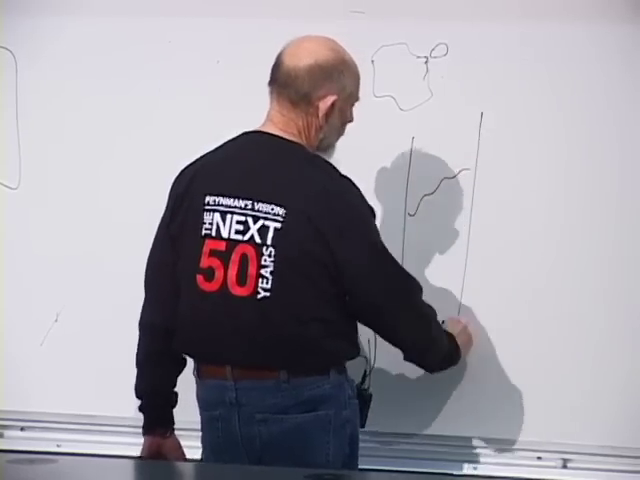
\includegraphics[width=0.72\textwidth]{lecture_06_figure_03.png}
\caption{Завершённые на доске схемы обмена: константа связи приписывается при испускании и ещё раз при поглощении.}
\lectureframe{00:11:30.000}
\end{figure}

В струнно-теоретической версии фотон заменяется гравитоном, а электрический заряд — на \(g_s\). Один фактор сопровождает испускание, а другой — поглощение, так что сила гравитационного взаимодействия масштабируется как \(g_s^2\).

На больших расстояниях то же взаимодействие должно воспроизводить закон тяготения Ньютона,
\begin{equation}
F_{\mathrm{grav}}\sim G_N\frac{M_1M_2}{r^2}.
\end{equation}
Массы и обратноквадратичная зависимость описывают источники и распространение; здесь нам важен множитель связи, который их умножает.

\begin{figure}[htbp]
\centering
\begin{tikzpicture}[x=1cm,y=1cm]
  \node[font=\small\bfseries] at (1.8,3.55) {electromagnetism};
  \draw[line width=0.8pt] (0,0) -- (0,3);
  \draw[line width=0.8pt] (3.6,0) -- (3.6,3);
  \draw[line width=0.8pt] plot[smooth] coordinates {(0,1.5) (0.45,1.72) (0.9,1.28) (1.35,1.72) (1.8,1.28) (2.25,1.72) (2.7,1.28) (3.15,1.72) (3.6,1.5)};
  \node[below] at (0,1.42) {\(e\)};
  \node[below] at (3.6,1.42) {\(e\)};
  \node[font=\small] at (1.8,0.25) {exchange strength \(\propto e^2\)};
  \node[font=\small\bfseries] at (7.2,3.55) {string gravity};
  \draw[line width=0.8pt,rounded corners=6pt] (5.4,0) -- (5.2,0.7) -- (5.5,1.5) -- (5.25,2.3) -- (5.4,3);
  \draw[line width=0.8pt,rounded corners=6pt] (9,0) -- (9.2,0.7) -- (8.9,1.5) -- (9.15,2.3) -- (9,3);
  \draw[line width=0.8pt] plot[smooth] coordinates {(5.5,1.5) (5.95,1.72) (6.4,1.28) (6.85,1.72) (7.3,1.28) (7.75,1.72) (8.2,1.28) (8.65,1.72) (8.9,1.5)};
  \node[below] at (5.5,1.42) {\(g_s\)};
  \node[below] at (8.9,1.42) {\(g_s\)};
  \node[font=\small] at (7.2,0.25) {exchange strength \(\propto g_s^2\)};
\end{tikzpicture}
\caption{Аналогия для подсчёта степеней константы связи. Каждый конец обмениваемого кванта даёт по одному фактору взаимодействия.}
\end{figure}

Это наблюдение почти определяет постоянную Ньютона. Константа связи \(g_s\) безразмерна, тогда как в четырёх измерениях \(G_N\) имеет размерность квадрата длины. Доступная микроскопическая длина — \(\ell_s\), поэтому
\begin{equation}
G_N\sim g_s^2\ell_s^2.
\label{eq:l06-newton-string}
\end{equation}
Объединяя это с уравнением~\eqref{eq:l06-planck-area}, получаем
\begin{equation}
\ell_p\sim g_s\ell_s.
\label{eq:l06-planck-string}
\end{equation}

\begin{figure}[htbp]
\centering
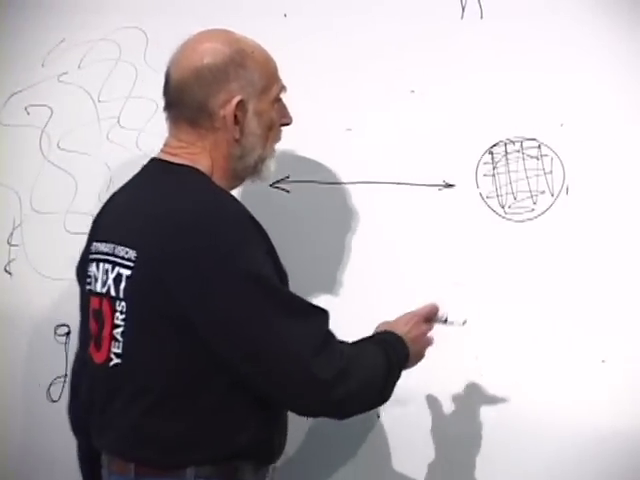
\includegraphics[width=0.72\textwidth]{lecture_06_figure_04.png}
\caption{Основные соотношения, оставленные на доске: \(\ell_p^2=G_N\) и \(\ell_p\sim g_s\ell_s\).}
\lectureframe{00:15:45.000}
\end{figure}

Уравнение~\eqref{eq:l06-newton-string} — это упрощённое соотношение, используемое на протяжении всей этой лекции.\editorialnote{В компактифицированной теории струн эффективная четырёхмерная постоянная Ньютона зависит также от объёма компактификации и от конвенций с коэффициентами порядка единицы. В лекции эти данные опускаются, чтобы выделить масштабирование соответствия.}

\begin{classroomqa}
\audiencequestion{Является ли \(g_s\) больше или меньше единицы, и какая длина больше?\lecturetimestamp{00:16:00}}
\lecturerresponse{Мы работаем при слабой связи, \(g_s<1\). Тогда из \(\ell_p\sim g_s\ell_s\) следует, что длина струны больше планковской длины. Сильная связь требует другого описания и здесь не нужна.}
\end{classroomqa}

\section{Подсчёт для чёрной дыры}

Опуская постоянную Больцмана и численные множители, энтропия Бекенштейна--Хокинга равна
\begin{equation}
S_{\mathrm{BH}}=\frac{A}{4G_N}sim\frac{A}{G_N}sim\frac{A}{\ell_p^2}.
\label{eq:l06-bh-area}
\end{equation}
Множитель \(1/4\) точен в полуклассической формуле, но в этом аргументе на уровне масштабирования он не играет роли.

\begin{classroomqa}
\audiencequestion{Указывает ли индекс ``BH'' на чёрную дыру или на Бекенштейна--Хокинга?\lecturetimestamp{00:16:51}}
\lecturerresponse{Для наших целей он может напоминать и об одном, и о другом. Важно то, что энтропия — это площадь горизонта, измеренная в единицах планковской площади.}
\end{classroomqa}

Для четырёхмерной чёрной дыры Шварцшильда,
\begin{equation}
R_s=2G_NM,
\qquad
A=4\pi R_s^2.
\end{equation}
Отбрасывая \(2\) и \(4\pi\), как это делается в лекции,
\begin{align}
S_{\mathrm{BH}}
&\sim \frac{R_s^2}{G_N}
\sim \frac{(G_NM)^2}{G_N} \\
&\sim M^2G_N
\sim M^2\ell_p^2.
\label{eq:l06-bh-mass}
\end{align}
Именно эту форму мы будем сравнивать со струнным подсчётом.

\section{Длинная струна как случайное блуждание}

Начнём с маленькой струны и будем закачивать в неё энергию. Типичная сильно возбуждённая струна не остаётся аккуратной петлёй. Она превращается в длинный запутанный объект, как леска на безнадёжно запутавшейся катушке. У этой путаницы есть энтропия, потому что огромное число конфигураций макроскопически выглядит одинаково.

Чтобы их подсчитать, заменим пространство решёткой, рёбра которой имеют длину \(\ell_s\). Узлы — это вершины, рёбра — линии, а элементарные квадраты — плакеты. Струна представляется связной последовательностью рёбер. Эта модель намеренно груба, но её экспоненциальный подсчёт состояний воспроизводит нужное масштабирование.

\begin{figure}[htbp]
\centering
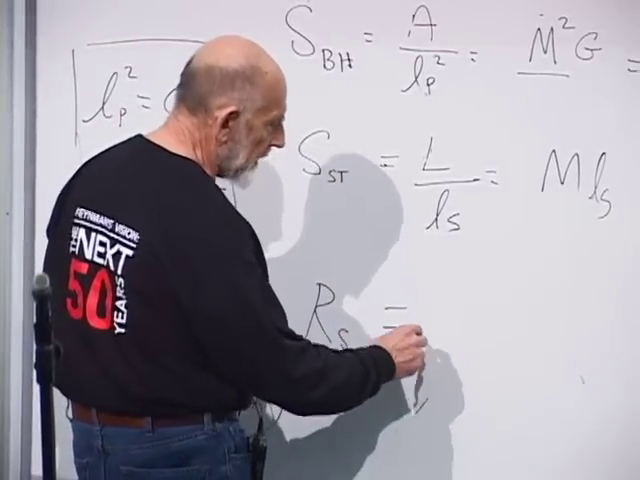
\includegraphics[width=0.72\textwidth]{lecture_06_figure_05.png}
\caption{Двумерная решёточная модель. Синий отрезок отмечает один шаг струны; в каждом узле учитываются все четыре возможных продолжения.}
\lectureframe{00:23:50.000}
\end{figure}

\begin{classroomqa}
\audiencequestion{Сколько вариантов есть на каждом шаге этого модельного блуждания?\lecturetimestamp{00:22:43}}
\lecturerresponse{Четыре на квадратной решётке, поскольку немедленный шаг назад разрешён. В трёх измерениях их было бы шесть. Другая решётка изменит конкретное число, но не тот факт, что число блужданий растёт экспоненциально с числом рёбер.}
\end{classroomqa}

Если у струны \(n\) рёбер, то двумерный модельный подсчёт даёт
\begin{equation}
\Omega_n\sim4^n.
\label{eq:l06-walk-count}
\end{equation}
Есть один исключительный прямой путь, но это лишь одно состояние среди \(4^n\). Типичный путь многократно складывается и образует запутанный клубок. При больших \(n\) почти каждая случайно сгенерированная конфигурация качественно похожа на любую другую.

Энтропия — это логарифм числа макроскопически неразличимых конфигураций:
\begin{equation}
S_{\mathrm{st}}=\log\Omega_n\sim n\log4\sim n.
\label{eq:l06-string-entropy-n}
\end{equation}

\begin{classroomqa}
\audiencequestion{Почему энтропия оказывается пропорциональной \(n\), а не \(4^n\)?\lecturetimestamp{00:25:39}}
\lecturerresponse{Энтропия есть логарифм числа состояний. Поэтому \(\log(4^n)=n\log4\), а множитель \(\log4\) — это константа порядка единицы, которую мы опустим.}
\end{classroomqa}

Если \(L\) — это контурная длина, получаемая, если проследить струну от одного конца до другого, то
\begin{equation}
n=\frac{L}{\ell_s},
\qquad
S_{\mathrm{st}}\sim\frac{L}{\ell_s}.
\label{eq:l06-string-entropy-length}
\end{equation}
Здесь \(L\) — не диаметр спутанного клубка. Это значительно большее расстояние, измеряемое вдоль струны.

Теперь перейдём от контурной длины к массе. При \(c=\hbar=1\) масса имеет размерность обратной длины. Поэтому одно звено размера струны имеет массу порядка
\begin{equation}
m_{\mathrm{link}}\sim\frac{1}{\ell_s}.
\label{eq:l06-link-mass}
\end{equation}

\begin{classroomqa}
\audiencequestion{Почему масса одного звена должна масштабироваться как \(1/\ell_s\)?\lecturetimestamp{00:29:20}}
\lecturerresponse{В этих единицах масса имеет размерность обратной длины, и \(\ell_s\) — единственная доступная длина. Эквивалентно, натяжение струны порядка \(1/\ell_s^2\), умноженное на длину звена \(\ell_s\), даёт тот же результат.}
\end{classroomqa}

Тогда для полной струны имеем
\begin{equation}
M\sim n m_{\mathrm{link}}
\sim\frac{n}{\ell_s}
\sim\frac{L}{\ell_s^2},
\qquad
L\sim M\ell_s^2.
\label{eq:l06-string-mass}
\end{equation}
Подстановка в уравнение~\eqref{eq:l06-string-entropy-length} даёт
\begin{equation}
S_{\mathrm{st}}\sim M\ell_s.
\label{eq:l06-string-entropy-mass}
\end{equation}
Решёточное случайное блуждание не учитывает ограничений мирового листа и численных коэффициентов, но экспоненциальный рост спектра сильно возбуждённой струны даёт то же ведущее масштабирование.\editorialnote{Конструкция со случайным блужданием — это мнемоника для плотности струнных состояний на высоких уровнях, а не буквальная дискретизация фундаментальной струны.}

\section{Несовпадение, с которого начинается аргумент}

Теперь имеются два ответа
\begin{equation}
S_{\mathrm{BH}}\sim M^2\ell_p^2,
\qquad
S_{\mathrm{st}}\sim M\ell_s.
\label{eq:l06-two-entropies}
\end{equation}
Они похожи друг на друга, но при фиксированной массе и произвольной константе связи не равны. Выражение для чёрной дыры квадратично по \(M\); струнное выражение линейно. Нельзя просто объявить горячую струну чёрной дырой, не объяснив, как встречаются эти два режима.

\begin{figure}[htbp]
\centering
\includegraphics[width=0.78\textwidth]{lecture_06_figure_06.png}
\caption{Сопоставление на доске в чистом виде: энтропия чёрной дыры сверху, энтропия длинной струны снизу, а слева сохранены соотношения Планка--струны.}
\lectureframe{00:33:20.000}
\end{figure}

На этом лекция прервалась. Эта пауза полезна: несовпадение — не провал идеи, а указание на то, что нужно сравнивать одно и то же состояние, меняя силу гравитации.

\section{Поворачивая ручку константы связи}

Будем держать \(\ell_s\) фиксированной и представим, что \(g_s\) можно менять. При \(g_s=0\) струны не расщепляются и не сливаются, а гравитация исчезает, поскольку \(G_N\sim g_s^2\ell_s^2\). Тогда состояние с достаточно большой энергией представляет собой длинную слабо взаимодействующую струну.

Медленно увеличим \(g_s\). Струнные взаимодействия становятся возможными и, что важнее для данного рассуждения, гравитация усиливается.

\begin{classroomqa}
\audiencequestion{По мере увеличения \(g_s\) не состоит ли первый эффект просто в том, что струна распадается на более короткие струны?\lecturetimestamp{00:36:29}}
\lecturerresponse{Расщепление и слияние становятся возможными, но держите \(\ell_s\) фиксированной и прослеживайте состояние с высокой энтропией. Главный эффект состоит в том, что растёт \(G_N\), так что собственная гравитация длинной струны стягивает спутанный клубок внутрь.}
\end{classroomqa}

Объект сжимается и становится плотнее. Его гравитационная потенциальная энергия отрицательна, так что сжатие уменьшает его полную энергию и тем самым массу.

\begin{classroomqa}
\audiencequestion{Увеличивается или уменьшается энергия, когда собственная гравитация стягивает струну?\lecturetimestamp{00:37:48}}
\lecturerresponse{Она уменьшается. Энергия связи становится более отрицательной. Масса вдоль этого пути не обязана оставаться фиксированной, хотя мы продолжаем отслеживать то же самое состояние.}
\end{classroomqa}

В конце концов размер объекта становится сравнимым с его радиусом Шварцшильда. После этого естественным становится описание как чёрной дыры. Более сильное начальное возбуждение достигает этого условия при меньшей связи, потому что более массивному объекту нужна меньшая сила гравитации, чтобы образовать горизонт.

\begin{figure}[htbp]
\centering
\resizebox{0.95\linewidth}{!}{%
\begin{tikzpicture}[x=1cm,y=1cm,>=Latex]
  \draw[->,line width=0.9pt] (0,0) -- (11,0) node[right] {increasing \(g_s\)};
  \node[draw,rounded corners,align=center,minimum width=2.6cm,minimum height=1.15cm] at (1.8,1.5) {long excited string\\weak self-gravity};
  \node[draw,rounded corners,align=center,minimum width=2.6cm,minimum height=1.15cm] at (5.5,1.5) {correspondence point\\\(R_s\sim\ell_s\)};
  \node[draw,circle,align=center,minimum size=1.8cm] at (9.3,1.5) {black\\hole};
  \draw[->,line width=0.8pt] (3.15,1.5) -- (4.1,1.5) node[midway,above,font=\small] {contracts};
  \draw[->,line width=0.8pt] (6.9,1.5) -- (8.25,1.5);
  \node[font=\small,align=center] at (5.5,-0.65) {same family of states followed slowly;\\binding energy and mass may change};
\end{tikzpicture}
}
\caption{Путь соответствия при фиксированной \(\ell_s\). Обращение стрелки возвращает состояние чёрной дыры к состоянию длинной струны.}
\end{figure}

\begin{classroomqa}
\audiencequestion{Следует ли представлять \(g_s\) между нулём и единицей?\lecturetimestamp{00:40:18}}
\lecturerresponse{Да. Рассуждение остаётся в режиме слабой связи. Если \(g_s\) очень мало, то состояние должно быть соответственно очень массивным, прежде чем оно станет чёрной дырой. Нам не нужно входить в плохо контролируемый режим \(g_s>1\).}
\end{classroomqa}

В мысленном эксперименте это медленное изменение обратимо.

\begin{classroomqa}
\audiencequestion{Если снова уменьшать связь, пока гравитация больше не сможет удерживать чёрную дыру вместе, во что она превращается?\lecturetimestamp{00:41:37}}
\lecturerresponse{В длинную струну. При исчезающей гравитации всё в этой конструкции должно описываться струнными состояниями. Поворот ручки в одну сторону отображает струну в чёрную дыру; обратный поворот отображает чёрную дыру в струну.}
\end{classroomqa}

При фиксированной полной энергии и в фиксированном объёме доминирующей высокоэнтропийной конфигурацией по существу оказывается одна длинная струна, а не огромное число коротких струн. Это утверждение здесь не выводится. Оно следует из статистической механики струн вблизи режима Хагедорна и ещё будет рассмотрено.

\section{Что видит внешний наблюдатель}

Где находится струна, когда объект описывается как чёрная дыра? Во внешнем описании она не исчезает внезапно. Время Шварцшильда отодвигает кажущееся пересечение на сколь угодно позднее время, так что струнные степени свободы описываются как накапливающиеся на горизонте или вблизи него.

\begin{figure}[htbp]
\centering
\includegraphics[width=0.72\textwidth]{lecture_06_figure_07.png}
\caption{Сопоставление на доске между макроскопическим горизонтом, где структура на струнном масштабе образует лишь тонкий размытый слой, и меньшим горизонтом, радиус которого приближается к масштабу петли.}
\lectureframe{00:45:30.000}
\end{figure}

При \(R_s\gg\ell_s\) чёрная дыра макроскопична, а структура струнного масштаба образует лишь тонкий слой по сравнению с радиусом горизонта. По мере того как радиус уменьшается до \(\ell_s\), различие между гладкой чёрной дырой и протяжённой струной теряет смысл. Это внешнее описание с растянутым горизонтом; его не следует путать с координатно-независимым утверждением о том, что падающее внутрь вещество никогда не пересекает регулярный горизонт.\editorialnote{В лекции используется внешнее описание, знакомое по принципу дополнительности чёрных дыр. Выражение ``на горизонте'' обозначает степени свободы, различаемые внешним описанием, а не отдельный вывод их ковариантного местоположения.}

Переход происходит, когда
\begin{equation}
R_s\sim\ell_s.
\label{eq:l06-correspondence-radius}
\end{equation}
Ниже струнного масштаба геометрия Шварцшильда не может разрешить структуру, которая, как предполагается, должна поддерживать её. Петли флуктуируют прочь от предполагаемого горизонта, и состояние правильнее называть струной.

\section{Точка соответствия}

Подставим \(R_s\sim G_NM\) в уравнение~\eqref{eq:l06-correspondence-radius}:
\begin{equation}
G_NM\sim\ell_s.
\end{equation}
Затем подставим \(G_N\sim g_s^2\ell_s^2\):
\begin{equation}
M g_s^2\ell_s^2\sim\ell_s,
\qquad
M g_s^2\ell_s\sim1.
\label{eq:l06-correspondence-condition}
\end{equation}

\begin{figure}[htbp]
\centering
\includegraphics[width=0.72\textwidth]{lecture_06_figure_08.png}
\caption{Завершённая алгебра перехода на доске: \(R_s\sim\ell_s\) приводит к заключённому в рамку безразмерному условию \(Mg_s^2\ell_s\sim1\).}
\lectureframe{00:49:50.000}
\end{figure}

Один из слушателей заметил, к чему ведёт это условие. В точке соответствия,
\begin{align}
S_{\mathrm{BH}}
&\sim M^2\ell_p^2
\sim M^2g_s^2\ell_s^2 \\
&=(M\ell_s)(Mg_s^2\ell_s)
\sim M\ell_s
\sim S_{\mathrm{st}}.
\label{eq:l06-entropy-preview}
\end{align}

\begin{classroomqa}
\audiencequestion{Следует ли уже из этих уравнений, что энтропии чёрной дыры и струны становятся равными?\lecturetimestamp{00:50:18}}
\lecturerresponse{Да. Именно к этому и ведёт вычисление. Необходимые ингредиенты уже выписаны на доске, но в лекции их полное объединение откладывается, чтобы можно было внимательно проследить логику соответствия.}
\end{classroomqa}

Уравнение~\eqref{eq:l06-entropy-preview} — это однострочный алгебраический набросок, неявно содержащийся в этом обмене репликами. Оно устанавливает масштабирование, а не точный коэффициент \(1/4\). Для точных микроскопических совпадений требуются лучше контролируемые чёрные дыры и более детальные струнные конструкции.\editorialnote{Лекция останавливается до того, как уравнение~\eqref{eq:l06-entropy-preview} будет представлено как завершённый вывод. Оно выписано здесь, потому что аудитория явно распознаёт это равенство и все необходимые соотношения уже появились.}

\section{Почему энтропию можно перенести через соответствие}

Остаётся ещё один логический ингредиент. Предположим, что управляющий параметр, такой как магнитное поле или \(g_s\), изменяется достаточно медленно, при том что система изолирована, а эволюция обратима. Энергии, размеры и связанность могут меняться, но энтропия сохраняется:
\begin{equation}
\Delta S=0.
\label{eq:l06-adiabatic-entropy}
\end{equation}
Лекция связывает это с сохранением информации. Энтропия измеряет информацию, скрытую грубозернистым описанием; медленное обратимое изменение гамильтониана перестраивает состояния, не стирая этой информации.

\begin{classroomqa}
\audiencequestion{Требует ли постоянство энтропии, чтобы на этом пути не было фазового перехода?\lecturetimestamp{00:54:01}}
\lecturerresponse{Да, состояние должно быть возможно непрерывно прослеживать. У конечной системы не бывает строго неаналитического термодинамического фазового перехода того типа, который возникает при бесконечном объёме, и если изменение достаточно медленно, соответствие можно рассматривать как плавный кроссовер.}
\end{classroomqa}

Адиабатический здесь используется в более сильном, квазистатическом и обратимом смысле. Адиабатический, но необратимый процесс может порождать энтропию; существенны медленность и возможность отслеживать состояние.\editorialnote{Термодинамическое утверждение \(\Delta S=0\) требует обратимого адиабатического пути. В квантовомеханическом смысле соответствующая идея состоит в том, чтобы при изменении параметра следовать одному и тому же набору состояний без неконтролируемых переходов между уровнями.}

\begin{classroomqa}
\audiencequestion{Почему одна длинная струна должна иметь большую энтропию, чем несколько более коротких струн, несущих ту же суммарную массу?\lecturetimestamp{00:54:44}}
\lecturerresponse{Это противоречит интуиции, но явный подсчёт высокоэнергетических состояний в фиксированном объёме отдаёт предпочтение компоненте с длинной струной. Доказательство откладывается; для настоящего рассуждения нам нужно лишь то, что чёрная дыра соответствует струнному сектору максимальной энтропии, а не разреженному газу из очень большого числа коротких струн.}
\end{classroomqa}

Поэтому рабочая стратегия такова:
\begin{enumerate}
\item Начните с чёрной дыры массой \(M_0\) при константе связи \(g_{s,0}\).
\item Медленно уменьшайте \(g_s\), оставаясь в том же семействе состояний с высокой энтропией.
\item Остановитесь при \(R_s\sim\ell_s\), где описание в терминах чёрной дыры сменяется описанием в терминах длинной струны.
\item Подсчитайте число струнных состояний, используя \(S_{\mathrm{st}}\sim M\ell_s\).
\item Перенесите эту энтропию обратно по обратимому пути к исходной чёрной дыре.
\end{enumerate}

\begin{figure}[htbp]
\centering
\includegraphics[width=0.72\textwidth]{lecture_06_figure_09.png}
\caption{Принцип, оставленный на доске при изложении стратегии: адиабатическое изменение \(g_s\) не меняет \(S\).}
\lectureframe{00:56:40.000}
\end{figure}

Теория струн дала гораздо более точные подсчёты энтропии для заряженных, вращающихся, суперсимметричных, почти экстремальных и многомерных чёрных дыр. Обсуждение нейтральной шварцшильдовской дыры здесь — это грубый аргумент соответствия: он выявляет параметрическую плотность состояний и физический кроссовер, а не точную защищённую вырожденность.\editorialnote{Точное согласие наиболее убедительно для специальных чёрных дыр, у которых подсчёт состояний защищён при изменении константы связи. В настоящей лекции намеренно даётся простейшая версия с точностью до порядка величины.}

\begin{classroomqa}
\audiencequestion{Может ли состояние при выключении гравитации превратиться в две струны, а не ровно в одну?\lecturetimestamp{00:58:25}}
\lecturerresponse{Существует конечная вероятность того, что получится небольшое число длинных струн, и вариант с двумя, а не с одной, не меняет ведущего масштабирования энтропии. Изменило бы рассуждение дробление на огромный газ коротких струн; высокоэнергетический статистический подсчёт не благоприятствует такому исходу.}
\end{classroomqa}

Чёрная дыра — это максимум энтропии, который можно упаковать в область, а длинная струна — соответствующее высокоэнтропийное состояние в отсутствие гравитации. Теперь эти два описания связаны, но ещё не доведены до точного расчёта. Следующий шаг — аккуратно повторить алгебру и спросить, насколько далеко можно доверять этому соответствию.

\chapter{Энтропия чёрных дыр, голография и пространство де Ситтера}

\lectureoverview{Мы завершаем аргумент соответствия, начатый на предыдущей лекции. Сильно возбуждённая струна обладает энтропией, пропорциональной её массе, тогда как шварцшильдовская чёрная дыра обладает энтропией, пропорциональной её площади. Эти две формулы связаны не отождествлением сильно гравитирующей чёрной дыры со свободной струной, а медленным изменением струнной константы связи до тех пор, пока эти два описания не встретятся. Затем закон площади естественным образом приводит к голографическому принципу, а в заключительной части лекции вводятся расширяющееся пространство и геометрия де Ситтера, горизонт которой будет изучаться далее.}

\section{Возвращение к задаче подсчёта}

В подсчёте для длинной струны оставалась одна недоговорённость. Если фиксированная полная длина распределена между несколькими струнами, то одинаковые струны одной и той же длины неразличимы. Тем не менее их положения в ящике входят в состояние, а сам ящик выбирается примерно того размера, который занимает соответствующая одиночная длинная струна.

\begin{classroomqa}
\audiencequestion{Различаются ли короткие струны между собой, и учитываются ли их положения?\lecturetimestamp{00:00:37}}
\lecturerresponse{Струны с одинаковыми свойствами неразличимы, но их положения в ящике учитываются. Сравнение проводится при фиксированном объёме, выбранном так, чтобы он совпадал с областью, занимаемой длинной струной.}
\end{classroomqa}

После этого можно сформулировать цель. Мы соберём короткий список уравнений и используем его, чтобы получить масштабное поведение энтропии чёрной дыры. Не потребуется ни интеграл, ни бесконечная сумма. Трудность не алгебраическая; она состоит в том, чтобы знать, какие величины можно сравнивать и на каком этапе рассуждения.

\section{Натуральные единицы и планковская площадь}

Положим
\begin{equation}
c=\hbar=1,
\label{eq:l07-natural-units}
\end{equation}
но оставим ньютоновскую постоянную в явном виде. Первое следствие состоит в том, что время и длина имеют одинаковые размерности. Соотношение для фотона
\begin{equation}
E=\frac{\hbar c}{\lambda}
\end{equation}
и соотношение массы и энергии \(E=mc^2\) тогда дают
\begin{equation}
[M]=L^{-1}.
\label{eq:l07-mass-dimension}
\end{equation}
Следовательно, массу можно выражать как обратную длину.

\begin{figure}[htbp]
\centering
\includegraphics[width=0.62\textwidth]{lecture_07_figure_02.png}
\caption{Соглашение о натуральных единицах в начале рассуждения о размерностях. Формула для энергии дополняется уравнениями, приведёнными выше.}
\lectureframe{00:03:27.900}
\end{figure}

Чтобы определить размерность \(G_N\), используем ньютоновское ускорение только как средство учёта размерностей:
\begin{equation}
a\sim\frac{G_NM}{R^2}.
\end{equation}
Поскольку \(T\) и \(L\) имеют одинаковую размерность, \([a]=L/T^2=L^{-1}\). Вместе с уравнением~\eqref{eq:l07-mass-dimension} это даёт
\begin{equation}
[G_N]=L^2.
\end{equation}
В этих единицах ньютоновская постоянная имеет размерность площади. Определяя планковскую длину как
\begin{equation}
G_N=\ell_p^2,
\label{eq:l07-planck-area}
\end{equation}
мы сразу понимаем, почему \(A/G_N=A/\ell_p^2\) безразмерно: оно измеряет площадь в единицах планковской площади.

\section{Струнная константа связи и сила гравитации}

Теперь гравитацию нужно перевести на язык струн. Полезная картина — это процесс обмена. Когда струна самопересекается, она может расщепиться и вновь соединиться. Маленькая петля замкнутой струны может быть испущена одним объектом и поглощена другим; когда это возбуждение является гравитоном, процесс опосредует гравитацию. Один множитель взаимодействия возникает при испускании, а другой — при поглощении, так что сила обмена содержит \(g_s^2\).

Константа связи \(g_s\) безразмерна. Точнее, это константа связи на уровне амплитуды, тогда как вероятность или скорость процесса начинается с порядка \(g_s^2\).\editorialnote{В лекции \(g_s\) иногда называется вероятностью, а затем это исправляется на квадратный корень из вероятности. Пертурбативная константа связи относится к уровню амплитуды.} Поскольку \(G_N\) имеет размерность площади, всё ещё не хватает масштаба длины. Его даёт фундаментальная струнная длина \(\ell_s\), масштаб одного элементарного колебания струны:
\begin{equation}
G_N\sim g_s^2\ell_s^2,
\qquad
\ell_p\sim g_s\ell_s.
\label{eq:l07-planck-string}
\end{equation}

\begin{figure}[htbp]
\centering
\includegraphics[width=0.72\textwidth]{lecture_07_figure_05.png}
\caption{Соотношение для константы связи на доске: \(G_N=\ell_p^2\) и \(g_s^2\ell_s^2\sim\ell_p^2\).}
\lectureframe{00:12:15.000}
\end{figure}

При слабой связи, \(g_s\ll1\), планковская длина намного меньше струнной длины. Уменьшение \(g_s\) ослабляет гравитацию, оставляя элементарный струнный масштаб фиксированным.\editorialnote{Для эффективной четырёхмерной теории в \(G_N\) также входят данные компактификации и численные соглашения. В этом рассуждении о масштабах они считаются фиксированными и опускаются.}

\section{Подсчёт для длинной струны}

Энтропия подсчитывает элементарные выборы, необходимые для задания состояния. Заменим сильно возбуждённую струну блужданием по квадратной решётке. В каждой вершине следующее звено может быть направлено в одну из четырёх сторон. Описывать элементарный выбор как один выбор из четырёх возможностей или как два бинарных выбора меняет лишь константу порядка единицы. Существенно число шагов.

Если \(L\) — контурная длина струны, а каждый шаг имеет длину \(\ell_s\), то требуется
\begin{equation}
N=\frac{L}{\ell_s}
\end{equation}
шагов. Число блужданий растёт экспоненциально, схематически как \(\Omega_N\sim q^N\), где \(q\) имеет порядок единицы, и потому
\begin{equation}
S_{\mathrm{str}}=\log\Omega_N\sim N\sim\frac{L}{\ell_s}.
\label{eq:l07-string-entropy-length}
\end{equation}

\begin{figure}[htbp]
\centering
\includegraphics[width=0.68\textwidth]{lecture_07_figure_03.png}

\vspace{0.7em}
\begin{tikzpicture}[scale=0.82]
  \draw[step=0.8cm,gray!45,thin] (0,0) grid (6.4,4.0);
  \draw[very thick,blue!60!black]
    (0.8,0.8)--(1.6,0.8)--(1.6,1.6)--(2.4,1.6)--(2.4,2.4)--
    (3.2,2.4)--(3.2,1.6)--(4.0,1.6)--(4.0,2.4)--(4.8,2.4)--
    (4.8,3.2)--(5.6,3.2);
  \draw[<->,thick] (0.8,-0.35)--(1.6,-0.35);
  \node[below] at (1.2,-0.35) {step \(\ell_s\)};
  \node[align=center] at (8.1,2.0) {\(N=L/\ell_s\) steps\\[0.3em]\(S_{\mathrm{str}}\sim N\)};
\end{tikzpicture}
\caption{Решёточная модель на доске и её приведённая в порядок интерпретация как случайного блуждания. Число выборов определяется контурной длиной, а не диаметром спутанного клубка.}
\lectureframe{00:17:20.000}
\end{figure}

Масса также подсчитывается по тем же элементарным сегментам. Сегмент длины \(\ell_s\) имеет масштаб массы
\begin{equation}
m_{\mathrm{seg}}\sim\frac{1}{\ell_s}.
\end{equation}

\begin{classroomqa}
\audiencequestion{Элементарному сегменту приписывается длина \(\ell_s\)?\lecturetimestamp{00:18:56}}
\lecturerresponse{Да. Его характерная длина равна \(\ell_s\), поэтому в натуральных единицах его характерная масса равна \(1/\ell_s\).}
\end{classroomqa}

Складывая массы \(L/\ell_s\) сегментов, получаем
\begin{equation}
M\sim\frac{L}{\ell_s}\frac{1}{\ell_s}
=\frac{L}{\ell_s^2},
\qquad
L\sim M\ell_s^2.
\label{eq:l07-string-mass}
\end{equation}
Кинетическая и потенциальная энергии колеблющейся струны здесь сжаты в это масштабное соотношение; более подробное статистико-механическое рассмотрение даёт ту же зависимость. Подстановка в уравнение~\eqref{eq:l07-string-entropy-length} приводит к формуле для струны, которая нам понадобится:
\begin{equation}
S_{\mathrm{str}}\sim M\ell_s.
\label{eq:l07-string-entropy-mass}
\end{equation}

\begin{figure}[htbp]
\centering
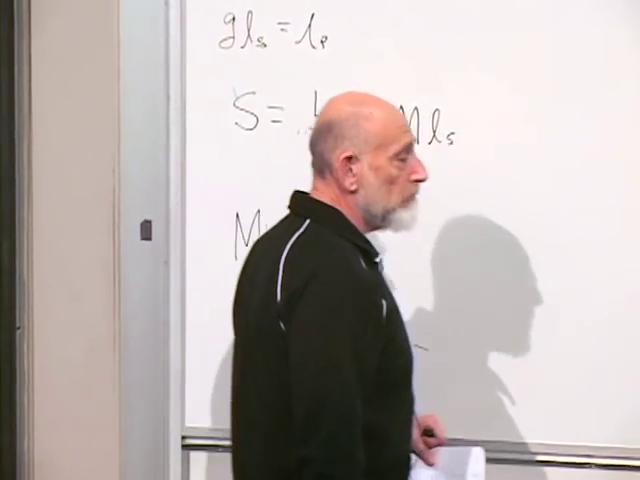
\includegraphics[width=0.66\textwidth]{lecture_07_figure_04.png}
\caption{Столбец со струнной стороны, собранный перед сравнением: \(\ell_p\sim g_s\ell_s\), \(S_{\mathrm{str}}\sim L/\ell_s\sim M\ell_s\) и \(M\sim L/\ell_s^2\).}
\lectureframe{00:21:57.800}
\end{figure}

\section{Почему свободная струна — это ещё не чёрная дыра}

Со стороны гравитации точная полуклассическая формула имеет вид
\begin{equation}
S_{\mathrm{BH}}=\frac{A}{4G_N}.
\label{eq:l07-bh-exact}
\end{equation}

\begin{classroomqa}
\audiencequestion{Какой численный коэффициент должен стоять в знаменателе?\lecturetimestamp{00:23:28}}
\lecturerresponse{Четыре. Аргумент соответствия восстановит масштабную зависимость, но он слишком груб, чтобы определить этот точный множитель.}
\end{classroomqa}

Для четырёхмерной шварцшильдовской чёрной дыры
\begin{equation}
R_s=2G_NM,
\qquad
A=4\pi R_s^2.
\end{equation}
Если, как в лекции, опустить численные множители,
\begin{align}
S_{\mathrm{BH}}
&\sim\frac{A}{G_N}
\sim\frac{(G_NM)^2}{G_N} \\
&\sim M^2G_N
\sim M^2\ell_p^2.
\label{eq:l07-bh-scaling}
\end{align}

\begin{figure}[htbp]
\centering
\includegraphics[width=0.72\textwidth]{lecture_07_figure_06.png}
\caption{Завершённое сравнение на доске: струнная энтропия — это длина в струнных единицах, тогда как энтропия чёрной дыры — площадь в планковских единицах.}
\lectureframe{00:25:35.000}
\end{figure}

Сходство между уравнениями~\eqref{eq:l07-string-entropy-mass} и \eqref{eq:l07-bh-scaling} наводит на мысль о связи, но это не одна и та же формула. Было бы неверно просто назвать исходную чёрную дыру свободной струной и выполнить подстановку. Подсчёт для свободной струны не учитывает притяжение между частями струны — именно то взаимодействие, которое сжимает её в чёрную дыру и понижает её полную энергию за счёт отрицательной энергии связи.

Ошибка хорошо знакома по примеру звезды. Горячий газ звёздной массы, помещённый в слишком большой ящик, не является моделью звезды, даже при той же температуре. Самогравитация изменяет равновесный размер и связь между энергией и энтропией. Отслеживать каждое самовзаимодействие длинной струны было бы трудно, поэтому мы не будем этого делать.

\begin{classroomqa}
\audiencequestion{Если от длинной струны отделяется маленькая петля, её энтропия уменьшается. Означает ли это, что обмен гравитонами понижает энтропию гравитирующей системы?\lecturetimestamp{00:28:48}}
\lecturerresponse{Нет, не в том равновесном обменном процессе, который используется здесь. Виртуальные возбуждения испускаются и поглощаются в обоих направлениях; эта схема не означает буквальную потерю постоянного фрагмента струны. Единственная цель этой схемы здесь — установить два множителя связи и, следовательно, зависимость от \(g_s^2\).}
\end{classroomqa}

\section{Адиабатическая игра соответствия}

Вместо этого начнём там, где гравитацией можно пренебречь. При \(g_s\to0\) струны пересекаются, не расщепляясь и не соединяясь, и самогравитационное притяжение исчезает. Увеличивайте \(g_s\), удерживая \(\ell_s\) фиксированным: гравитация усиливается, сильно возбуждённая струна сжимается и в конце концов становится чёрной дырой. Медленно поверните этот параметр обратно, и чёрная дыра должна вернуться в струнное состояние. Она может перейти в небольшое число длинных струн, но подсчёт состояний при высоких энергиях из предыдущей лекции говорит, что доминирующий сектор содержит одну длинную струну, а не огромный газ из коротких.

\begin{classroomqa}
\audiencequestion{Что удерживается фиксированным при изменении константы связи?\lecturetimestamp{00:32:19}}
\lecturerresponse{Фиксированной удерживается струнная длина \(\ell_s\), а значит и элементарный струнный масштаб массы \(1/\ell_s\). Регулятор изменяет \(g_s\) и, следовательно, \(G_N\sim g_s^2\ell_s^2\).}
\end{classroomqa}

Изменение должно быть медленным, изолированным и обратимым. При этих условиях энтропия является адиабатическим инвариантом:
\begin{equation}
\Delta S=0.
\label{eq:l07-adiabatic}
\end{equation}
Одной лишь медленности недостаточно, если происходят диссипативные или неконтролируемые переходы. Здесь ``адиабатический'' означает, что одно и то же семейство состояний можно непрерывно прослеживать.\editorialnote{Это термодинамический смысл адиабатичности, связанный с обратимыми процессами. Необратимый процесс может быть адиабатическим в смысле отсутствия теплопередачи и всё же производить энтропию.}

Пусть рассматриваемая чёрная дыра имеет массу \(M_0\) и константу связи \(g_{s,0}\). До использования формулы площади, которую мы пытаемся объяснить, анализ размерностей говорит лишь, что энтропия нейтральной невращающейся чёрной дыры является некоторой функцией безразмерной комбинации
\begin{equation}
S_{\mathrm{BH}}=f(M\ell_p)
=f(Mg_s\ell_s).
\label{eq:l07-entropy-function}
\end{equation}
При фиксированной \(\ell_s\) изоэнтропический путь, следовательно, сохраняет
\begin{equation}
Mg_s=M_0g_{s,0}
\label{eq:l07-adiabat}
\end{equation}
постоянной, при условии что прослеживается одна и та же ветвь состояний.

По мере уменьшения \(g_s\) отрицательная энергия связи устраняется, так что масса \(M\) вдоль этого пути возрастает. Соответствующая струнная конфигурация тоже становится менее тесно связанной и расплывается. Однако формальный радиус Шварцшильда на адиабате ведёт себя как \(R_s\sim Mg_s^2\ell_s^2\sim g_s\ell_s\) и потому уменьшается.\editorialnote{В устном обсуждении к объекту, освобождаемому от гравитационной связи, применяется слово ``растёт''. Это не следует понимать так, будто радиус Шварцшильда вдоль выведенной адиабаты увеличивается.}

\begin{classroomqa}
\audiencequestion{Увеличивается объект или уменьшается по мере ослабления гравитации?\lecturetimestamp{00:36:28}}
\lecturerresponse{Его струнная структура высвобождается и расширяется, тогда как масса увеличивается, поскольку отрицательная энергия связи устраняется. Радиус, приписываемый формулой чёрной дыры, уменьшается, пока не достигает струнного масштаба, где такое описание в терминах чёрной дыры перестаёт быть полезным.}
\end{classroomqa}

\section{Две кривые и их пересечение}

Отложим массу по вертикали, а струнную константу связи — по горизонтали. Уравнение ~\eqref{eq:l07-adiabat} задаёт гиперболу, \(M\propto g_s^{-1}\).

\begin{classroomqa}
\audiencequestion{Какой вид имеет кривая с постоянным произведением \(Mg_s\)?\lecturetimestamp{00:44:08}}
\lecturerresponse{Гипербола. Это адиабата, проходящая через рассматриваемую точку \((g_{s,0},M_0)\).}
\end{classroomqa}

Вторая кривая отмечает кроссовер между описаниями. Чёрную дыру уже нельзя разрешить как обычную геометрию Шварцшильда, когда её радиус меньше элементарного колебания струны. Поэтому точку соответствия мы оцениваем из условия
\begin{equation}
R_s\sim\ell_s.
\label{eq:l07-correspondence-radius}
\end{equation}
Используя \(R_s\sim MG_N\) и уравнение ~\eqref{eq:l07-planck-string}, получаем
\begin{equation}
Mg_s^2\ell_s^2\sim\ell_s,
\qquad
Mg_s^2\sim\frac{1}{\ell_s}.
\label{eq:l07-transition-curve}
\end{equation}
Таким образом, кривая перехода убывает как \(M\propto g_s^{-2}\), круче, чем адиабата.

\begin{figure}[htbp]
\centering
\includegraphics[width=0.70\textwidth]{lecture_07_figure_07.png}

\vspace{0.6em}
\begin{tikzpicture}[x=1cm,y=0.78cm]
  \draw[->] (0.4,0.4)--(7.0,0.4) node[right] {\(g_s\)};
  \draw[->] (0.4,0.4)--(0.4,6.5) node[above] {\(M\)};
  \draw[thick,black] plot[smooth] coordinates {(1.0,5.6) (1.5,4.0) (2.2,2.9) (3.2,2.1) (4.6,1.55) (6.3,1.2)};
  \draw[very thick,red!70!black] plot[smooth] coordinates {(1.25,6.0) (1.55,4.55) (2.0,3.15) (2.7,2.0) (3.8,1.25) (5.8,0.78)};
  \fill (2.05,3.1) circle (2pt) node[above right] {\((g_{s,*},M_*)\)};
  \node[black,rotate=-17] at (4.75,1.9) {\(Mg_s=M_0g_{s,0}\)};
  \node[red!70!black,rotate=-25] at (4.45,0.95) {\(Mg_s^2=1/\ell_s\)};
  \node at (5.75,3.5) {black hole};
  \node at (1.15,1.25) {string};
\end{tikzpicture}
\caption{График с доски и его аккуратная интерпретация. Чёрная адиабата пересекает более крутую красную кривую соответствия в точке, где объект становится струноподобным.}
\lectureframe{00:49:35.000}
\end{figure}

В точке пересечения \((M_*,g_{s,*})\) два уравнения имеют вид
\begin{align}
M_*g_{s,*} &= M_0g_{s,0}, \\
M_*g_{s,*}^2 &\sim \frac{1}{\ell_s}.
\end{align}
Возведём первое уравнение в квадрат и разделим на второе:
\begin{equation}
M_*
\sim M_0^2g_{s,0}^2\ell_s.
\end{equation}
Умножая на \(\ell_s\),
\begin{equation}
M_*\ell_s
\sim M_0^2g_{s,0}^2\ell_s^2
\sim M_0^2G_{N,0}.
\label{eq:l07-crossover-result}
\end{equation}

\begin{figure}[htbp]
\centering
\includegraphics[width=0.68\textwidth]{lecture_07_figure_08.png}
\caption{Завершённая алгебра перехода, включая \(M_*\ell_s=M_0^2g_{s,0}^2\ell_s^2=M_0^2G_{N,0}\).}
\lectureframe{00:54:40.000}
\end{figure}

\begin{classroomqa}
\audiencequestion{После деления уравнений двух кривых \(\ell_s\) должно оказаться в числителе или в знаменателе?\lecturetimestamp{00:52:41}}
\lecturerresponse{В числителе. Деление на \(1/\ell_s\) равносильно умножению на \(\ell_s\), поэтому \(M_*\sim M_0^2g_{s,0}^2\ell_s\).}
\end{classroomqa}

В точке перехода применима струнная формула, так что
\begin{equation}
S_*\sim M_*\ell_s.
\end{equation}
Энтропия вдоль пути не изменялась. Сочетая это утверждение с уравнением ~\eqref{eq:l07-crossover-result}, получаем энтропию исходной чёрной дыры:
\begin{equation}
S_{\mathrm{BH}}(M_0)
\sim M_0^2G_{N,0}
\sim M_0^2\ell_{p,0}^2.
\label{eq:l07-final-correspondence}
\end{equation}
Это и есть искомое масштабирование по закону площади.

\section{Что соответствие доказывает и чего не доказывает}

Эта конструкция не утверждает, что исходная, сильно гравитирующая чёрная дыра является свободной струной. Она переводит объект в режим, где подсчёт струнных состояний надёжен, считывает там энтропию и переносит её обратно вдоль обратимого пути. Переход является кроссовером, а не резко локализованной фазовой границей, поэтому эта оценка не может определить коэффициент \(1/4\) в уравнении ~\eqref{eq:l07-bh-exact}.

Тем не менее та же логика работает на уровне параметрических оценок для заряженных чёрных дыр, чёрных объектов в других размерностях и протяжённых чёрных бран. Более симметричные и суперсимметричные примеры допускают защищённые подсчёты состояний, сохраняющие точную информацию при изменении константы связи; эти методы восстанавливают численные коэффициенты, но вводят математический аппарат, не нужный для настоящего концептуального аргумента.

Наиболее важно то, что это вычисление даёт микроскопическую интерпретацию. Энтропия служит свидетельством скрытой структуры. Гидродинамика описывает плотность, давление и течение, не упоминая молекулы; энтропия жидкости показывает, что такие микроскопические степени свободы существуют. Общая теория относительности аналогично описывает горизонт, не показывая его микросостояния. Подсчёт струнных состояний показывает, что непротиворечивая квантовая теория гравитации может содержать достаточно состояний, чтобы объяснить энтропию чёрной дыры.

\begin{classroomqa}
\audiencequestion{Что означало бы \(S\sim M^3\ell_p^3\) вместо квадратичного результата?\lecturetimestamp{00:59:41}}
\lecturerresponse{Это выглядело бы как закон объёма. Обычное вещество в комнате или чашке кофе имеет энтропию, пропорциональную объёму; квадратичный ответ особенный, потому что через \(R_s\sim M\ell_p^2\) он пропорционален площади горизонта.}
\end{classroomqa}

Этот результат свидетельствует о том, что энтропия Бекенштейна--Хокинга — не просто формальная термодинамическая аналогия. Он указывает на микроскопические гравитационные степени свободы, хотя элементарный вывод не делает эти степени свободы видимыми по отдельности.

\section{От максимальной энтропии к голографии}

Теперь мы меняем вопрос. Вместо того чтобы спрашивать об энтропии заданного состояния, спросим о наибольшей энтропии, совместимой с данной областью.

Начнём с обычной решёточной модели комнаты. Разобьём объём на ячейки размера \(V_{\mathrm{cell}}\), и пусть каждой ячейке соответствует один вопрос с ответом да или нет: занята или пуста. Сасскинд даёт воображаемому атому нарочито нелепое название ``мясоний'', чтобы никакие реалистические атомные детали не отвлекали от подсчёта. Если
\begin{equation}
N=\frac{V}{V_{\mathrm{cell}}},
\end{equation}
то число конфигураций и максимальная энтропия равны
\begin{equation}
\Omega=2^N,
\qquad
S_{\max}=\log\Omega=N\log2
\sim\frac{V}{V_{\mathrm{cell}}}.
\label{eq:l07-volume-count}
\end{equation}

\begin{figure}[htbp]
\centering
\includegraphics[width=0.68\textwidth]{lecture_07_figure_09.png}
\caption{Комната, разделённая на ячейки, с двумя состояниями на ячейку. Здесь подсчитывается максимальная энтропия, а не энтропия упорядоченной комнаты, занятой слушателями.}
\lectureframe{01:05:20.000}
\end{figure}

Реальная комната намного ниже этого максимума. Состояние, которое хаотически исследовало бы все эти варианты заполнения ячеек, было бы чрезвычайно горячим. От игрушечной модели сохраняется обычное ожидание, что число независимых степеней свободы, а следовательно и максимальная энтропия, масштабируются с объёмом.

Гравитация опровергает это ожидание. Рассмотрим сферическую область с площадью границы \(A\), начальной энтропией \(S_{\mathrm{i}}\) и массой \(M\), меньшей, чем масса \(M_{\mathrm{BH}}\) чёрной дыры, которая как раз заполнила бы сферу. Если бы \(M\) было больше, горизонт уже выходил бы за выбранную границу.

Теперь отправим внутрь оболочку массой \(M_{\mathrm{BH}}-M\). Её состав несущественен; в лекции допускаются свет, обычное вещество или даже швейцарский сыр. Устроим так, чтобы она сколлапсировала. Конечное состояние — чёрная дыра, горизонт которой как раз заполняет область, с энтропией
\begin{equation}
S_{\mathrm{f}}=\frac{A}{4G_N}.
\end{equation}
Второй закон требует
\begin{equation}
S_{\mathrm{i}}\le S_{\mathrm{f}}
=\frac{A}{4G_N}.
\label{eq:l07-holographic-bound}
\end{equation}

\begin{figure}[htbp]
\centering
\includegraphics[width=0.70\textwidth]{lecture_07_figure_10.png}

\vspace{0.5em}
\begin{tikzpicture}[scale=0.88]
  \draw[thick] (0,0) circle (1.35);
  \draw[very thick,red!70!black] (0,0) circle (2.05);
  \fill[gray!25] (0,0) circle (1.32);
  \node at (0,0) {\(M,S_{\mathrm{i}}\)};
  \draw[-{Latex[length=3mm]},thick,red!70!black] (3.5,0)--(2.15,0);
  \node[align=center,right] at (3.5,0) {incoming shell\\\(M_{\mathrm{BH}}-M\)};
  \node[below] at (0,-2.2) {final horizon area \(A\)};
\end{tikzpicture}
\caption{Конструкция с оболочкой. Внутрь посылается достаточно дополнительной массы, чтобы образовалась чёрная дыра, горизонт которой как раз заполняет выбранную область.}
\lectureframe{01:13:30.000}
\end{figure}

Поскольку чёрная дыра такого размера является допустимым состоянием и насыщает это неравенство, максимальная энтропия равна
\begin{equation}
S_{\max}=\frac{A}{4G_N}.
\label{eq:l07-holographic-maximum}
\end{equation}
Это и есть голографический принцип в его счётной формулировке: максимальное число независимых степеней свободы в гравитирующей области масштабируется с площадью её границы, приблизительно по одной степени свободы порядка единицы на каждую планковскую площадь, а не с числом заключённых внутри планковских объёмов.\editorialnote{Аргумент с оболочкой предполагает, что область можно охватить и заставить сколлапсировать указанным образом. Для более общих пространств-времён требуются ковариантные энтропийные ограничения, но сферический аргумент передаёт принцип, используемый в лекции.}

Несоответствие огромно. Интуиция локальной теории поля подсказывает, что выборы, сделанные в разных внутренних точках, должны комбинироваться независимо, давая закон объёма. Гравитация говорит, что достаточно большое число таких выборов само бы сколлапсировало, и чёрная дыра даёт большую допустимую энтропию. Поэтому граничный подсчёт — не малая поправка к объёмному; это иная организация гильбертова пространства.

\begin{classroomqa}
\audiencequestion{Что происходит для очень большой Вселенной с примерно однородной плотностью?\lecturetimestamp{01:15:48}}
\lecturerresponse{Этот вопрос требует космологии, а не статической сферической конструкции. Именно он мотивирует немедленный переход к расширяющимся решениям уравнений Эйнштейна.}
\end{classroomqa}

\begin{classroomqa}
\audiencequestion{Связано ли ограничение по площади с принципом неопределённости?\lecturetimestamp{01:16:03}}
\lecturerresponse{Лекция оставляет этот вопрос открытым и затем переходит к космологии.}
\end{classroomqa}

\section{Расширяющееся пространство}

Мы не будем здесь выводить космологические решения из уравнений Эйнштейна; мы просто запишем решения и научимся их читать. Пространственные срезы могут быть положительно искривлёнными и замкнутыми, отрицательно искривлёнными и гиперболическими или плоскими. В дальнейшем обсуждении возьмём пространственно-плоские евклидовы срезы в нестационарном пространстве-времени.

\begin{classroomqa}
\audiencequestion{Каков пространственно-временной аналог обычного евклидова пространства?\lecturetimestamp{01:19:37}}
\lecturerresponse{Пространство Минковского. Рассматриваемая здесь космологическая модель имеет плоские пространственные срезы, но не является пространством-временем Минковского, поскольку её пространственная метрика меняется со временем.}
\end{classroomqa}

Знакомая картинка с воздушным шаром описывает замкнутую расширяющуюся поверхность размерностью на единицу меньше. Susskind вспоминает, как пытался провести эту демонстрацию с большим размеченным шаром; маркер ослабил резину и привёл к буквальному хлопку. Этот случай также обнаруживает концептуальный изъян аналогии. Когда обычный шарик расширяется, молекулы резины расходятся, и материал истончается, пока не рвётся. В космологическом пространстве локальные законы не размываются. Чтобы сохранить аналогию, нужно воображать, что всё новые молекулы резины непрерывно вставляются, так что каждый малый участок сохраняет одни и те же локальные свойства. В плоской модели замените шарик большим листом, который равномерно растягивают наружу и так же пополняют новым материалом.

Математически расширение входит в метрику:
\begin{equation}
\begin{aligned}
ds^2&=-dt^2+a(t)^2d\mathbf{x}^2,\\
d\mathbf{x}^2&=\delta_{ij}\,dx^i dx^j
=dx^2+dy^2+dz^2.
\end{aligned}
\label{eq:l07-frw-metric}
\end{equation}

\begin{figure}[htbp]
\centering
\includegraphics[width=0.72\textwidth]{lecture_07_figure_11.png}
\caption{Пространственно-плоская расширяющаяся метрика, записанная на доске.}
\lectureframe{01:25:10.000}
\end{figure}

Точки, сохраняющие фиксированные пространственные координаты, называются сопутствующими. Если две такие точки имеют координатное расстояние \(\Delta x\), то их собственное расстояние в момент \(t\) равно
\begin{equation}
D(t)=a(t)\Delta x.
\label{eq:l07-proper-distance}
\end{equation}
Их координаты не меняются, но метрическое расстояние между ними меняется. Дифференцируя при фиксированном \(\Delta x\),
\begin{equation}
V=\dot D=\dot a\,\Delta x
=\frac{\dot a}{a}D.
\end{equation}
Введём параметр Хаббла
\begin{equation}
H(t)=\frac{\dot a(t)}{a(t)}.
\label{eq:l07-hubble-parameter}
\end{equation}
Тогда
\begin{equation}
V=H(t)D,
\label{eq:l07-hubble-law}
\end{equation}
что и есть закон Хаббла при фиксированном космическом времени.

\begin{figure}[htbp]
\centering
\includegraphics[width=0.68\textwidth]{lecture_07_figure_12.png}
\caption{Записанный на доске закон удаления при фиксированном времени: \(V=D\,\dot a/a\).}
\lectureframe{01:29:10.000}
\end{figure}

Название ``постоянная Хаббла'' может вводить в заблуждение. Вообще говоря, \(H(t)\) меняется со временем. Пространственно постоянным является отношение \(V/D\) для любой пары сопутствующих точек на одном и том же временном срезе.

\begin{classroomqa}
\audiencequestion{Для далёких галактик чьё время входит в это соотношение? Мы наблюдаем их на более ранней эпохе.\lecturetimestamp{01:31:10}}
\lecturerresponse{Уравнение~\eqref{eq:l07-hubble-law} относится к одновременному срезу. Наблюдение идёт вдоль направленного в прошлое светового луча и фиксирует далёкую галактику в более ранний момент, поэтому связь между измеренным красным смещением и расстоянием требует всей истории вдоль светового конуса, а не одного мгновенного значения \(H\).}
\end{classroomqa}

\begin{figure}[htbp]
\centering
\includegraphics[width=0.66\textwidth]{lecture_07_figure_13.png}
\caption{Пространственно-временной рисунок, используемый, чтобы отличить расстояние на срезе равного времени от того, что наблюдатель видит вдоль направленного в прошлое светового луча.}
\lectureframe{01:33:20.000}
\end{figure}

\section{Масштаб Хаббла и расширение де Ситтера}

В единицах \(c=1\) уравнение~\eqref{eq:l07-hubble-law} даёт скорость удаления, равную единице, на расстоянии
\begin{equation}
D_H=\frac{1}{H}.
\label{eq:l07-hubble-radius}
\end{equation}
Более удалённые сопутствующие точки могут иметь \(V>1\) или даже \(V\gg1\), не нарушая специальную теорию относительности. Они не пролетают мимо локального наблюдателя быстрее света; их собственное расстояние растёт, потому что расширяется геометрия между ними.\editorialnote{В общей зависящей от времени космологии \(1/H\) — это радиус Хаббла, а не автоматически горизонт событий. Он становится постоянным масштабом горизонта в случае де Ситтера, обсуждаемом далее.}

Во многих старых замедляющихся космологических моделях \(H(t)\) уменьшается, а \(1/H(t)\) растёт, так что области, когда-то удалявшиеся сверхсветово, позднее могут войти в причинный контакт. Напротив, обсуждаемая в лекции картина на поздних временах стремится к положительной постоянной \(H\). Тогда \(1/H\) остаётся фиксированным, и уравнение расширения принимает вид
\begin{equation}
\frac{\dot a}{a}=H,
\qquad
\dot a=Ha.
\label{eq:l07-constant-h}
\end{equation}

\begin{classroomqa}
\audiencequestion{Каковы единицы измерения постоянного параметра Хаббла?\lecturetimestamp{01:38:24}}
\lecturerresponse{Обратное время. Эквивалентно, при \(c=1\) это обратная длина. Величина \(H^{-1}\) задаёт и время расширения, и масштаб расстояния; в лекции приводится пример порядка величины — около пятнадцати миллиардов лет.}
\end{classroomqa}

Решение уравнения~\eqref{eq:l07-constant-h} имеет вид
\begin{equation}
a(t)=a_0e^{Ht}.
\label{eq:l07-desitter-scale-factor}
\end{equation}

\begin{classroomqa}
\audiencequestion{Какая функция имеет скорость изменения, пропорциональную самой себе?\lecturetimestamp{01:39:04}}
\lecturerresponse{Экспонента. Следовательно, масштабный фактор равен \(a_0e^{Ht}\), тогда как пространственный коэффициент \(a(t)^2\) в метрике растёт как \(e^{2Ht}\).}
\end{classroomqa}

\begin{figure}[htbp]
\centering
\includegraphics[width=0.70\textwidth]{lecture_07_figure_14.png}
\caption{Уравнения при постоянном \(H\) и их экспоненциальное решение на доске.}
\lectureframe{01:39:30.000}
\end{figure}

Пространство-время с таким экспоненциальным расширением — это пространство де Ситтера. Его постоянный масштаб Хаббла задаёт горизонт событий на конечном собственном расстоянии. Эта геометрия в некотором смысле дополняет картину чёрной дыры: наблюдатель остаётся внутри космологического горизонта, тогда как достаточно далёкие объекты удаляются и уже никогда не смогут послать сигналы, которые достигнут его. Горизонт чёрной дыры скрывает внутреннюю область от внешнего наблюдателя; горизонт де Ситтера скрывает внешнюю часть области, доступной наблюдателю. В отличие от обычной испаряющейся чёрной дыры, идеальная геометрия де Ситтера рассматривается здесь как сохраняющаяся во времени. Здесь это сравнение только начинается. В следующей лекции подробнее рассматриваются горизонт, его термодинамика и загадки, которые он создаёт для космологии.

\chapter{Энергия вакуума и горизонты де Ситтера}

\lectureoverview{Энергия вакуума не похожа на обычную материю: она не выделяет предпочтённую инерциальную систему отсчёта и не разрежается по мере расширения Вселенной. Как только учитывается гравитация, этот на первый взгляд безобидный выбор нуля энергии изменяет геометрию пространства-времени. Мы выведем закон при доминировании материи \(a(t)\propto t^{2/3}\), сопоставим его с законом при доминировании вакуума \(a(t)\propto e^{Ht}\), а затем перепишем пространство-время де Ситтера в конформных координатах. Получающаяся причинная диаграмма обнаруживает зависящий от наблюдателя горизонт событий на фиксированном собственном расстоянии.}

\section{Квантовые флуктуации в вакууме}

Начнём с вопроса, который задаёт мотив всей лекции. Квантовая теория поля приписывает пустому пространству энергию. Означает ли это, что реальные электрон--позитронные пары непрерывно возникают из ничего?

\begin{classroomqa}
\audiencequestion{Происходят ли в вакууме в действительности рождение и аннигиляция электрон--позитронных пар, или это лишь удобный способ учёта?\lecturetimestamp{00:00:06}}
\lecturerresponse{Виртуальные пары вносят вклад в энергию вакуума, но это не обычные частицы, за появлением которых можно наблюдать в пустом пространстве. Они представляют собой флуктуации квантового основного состояния и существуют лишь в пределах, допустимых для виртуального процесса.}
\end{classroomqa}

Наиболее наглядную модель даёт гармонический осциллятор. Классически он может оставаться неподвижным в минимуме своего потенциала. Квантовомеханически точное положение в минимуме и точно нулевой импульс несовместимы. Основное состояние является компромиссом между этими двумя требованиями и сохраняет энергию нулевых колебаний
\begin{equation}
E_0=\frac{1}{2}\hbar\omega.
\label{eq:l08-zero-point}
\end{equation}
Это наименьшая энергия, которой может обладать осциллятор. Соответствующее состояние не является возбуждённым и не представляет собой поток наблюдаемых частиц.

Свободное поле разлагается на нормальные моды, каждая из которых ведёт себя как осциллятор. Электромагнитное поле в резонаторе — привычный пример. Каждая мода даёт вклад вида, указанного в уравнении~\eqref{eq:l08-zero-point}; электронное, кварковое и другие квантовые поля вносят собственные флуктуации основного состояния. Суммирование этих вкладов даёт то, что мы называем энергией вакуума. Печально известное несоответствие между наивными микроскопическими оценками и наблюдаемым космологическим масштабом реально, но оно не является темой этой лекции.

\begin{classroomqa}
\audiencequestion{Будет ли ещё обсуждаться расхождение примерно в \(120\) порядков величины?\lecturetimestamp{00:02:59}}
\lecturerresponse{Здесь — нет. Нынешняя цель состоит в том, чтобы понять космологические горизонты: как космологические уравнения приводят к ускоренному расширению и почему ускоренное расширение создаёт горизонты событий.}
\end{classroomqa}

\begin{classroomqa}
\audiencequestion{Является ли ультрафиолет--инфракрасное соотношение из прошлой лекции частью сегодняшнего обсуждения?\lecturetimestamp{00:03:59}}
\lecturerresponse{Возможно, мы вернёмся к нему позже, но в намеченную аргументацию оно не входит. Непосредственный путь ведёт от энергии вакуума к космологии, а затем к горизонтам.}
\end{classroomqa}

\section{Почему энергия вакуума инвариантна относительно преобразований Лоренца}

Следующий вопрос кажется элементарным, но выявляет определяющее свойство энергии вакуума. Если пустое пространство имеет положительную плотность энергии, почему оно не ведёт себя как оптическая среда и не изменяет скорость света?

\begin{classroomqa}
\audiencequestion{Не должна ли положительная плотность энергии вакуума оказывать преломляющее действие, заставляя свет распространяться немного медленнее?\lecturetimestamp{00:04:35}}
\lecturerresponse{Обычное вещество может делать это, потому что задаёт предпочтённую систему покоя. Энергия вакуума иная: она не выделяет такой системы, и каждый инерциальный наблюдатель получает одно и то же значение плотности энергии вакуума. Поэтому локальные измерения света сохраняют инвариантную скорость \(c\).}
\end{classroomqa}

Нужно различать симметрию законов и симметрию конкретного состояния. Уравнения физики могут быть инвариантны относительно трансляций, хотя Stanford — не Berkeley, а Земля — не межзвёздное пространство. Трансляция \emph{всей} физической конфигурации оставляет законы неизменными; реальное распределение материи не обязано выглядеть одинаково в каждой точке. Точно так же уравнения, инвариантные относительно вращений, не делают эту аудиторию вращательно симметричной.

То же различие относится и к преобразованиям Лоренца. У газа есть система покоя. Наблюдатель, движущийся относительно него, видит движущиеся молекулы и другую плотность энергии, так что состояние газа не лоренц-инвариантно, хотя управляющие им уравнения таковы. Обычное вещество, ванны излучения и лабораторная аппаратура — всё это нарушает симметрию, выделяя особые состояния движения или направления.

Энергия вакуума — особая форма материи, которая этого не делает. Представьте себе детектор, показывающий плотность энергии вакуума. В состоянии покоя он даёт некоторое значение \(\rho_{\rm vac}\). Разгоните детектор и повторите измерение: результат не изменится. В релятивистской записи это свойство выражается тензором энергии-импульса, пропорциональным метрике,
\begin{equation}
T_{\mu\nu}^{\rm vac}=-\rho_{\rm vac}g_{\mu\nu},
\qquad
p_{\rm vac}=-\rho_{\rm vac}.
\label{eq:l08-vacuum-stress}
\end{equation}
\editorialnote{Соотношение для давления на доске не выводится. Это ковариантная формулировка двух определяющих свойств, на которых строится лекция: лоренц-инвариантности и постоянной плотности при расширении.}

Локальная оговорка существенна. Для светового луча, проходящего мимо наблюдателя, измерения с помощью близлежащих часов и линеек дают скорость \(c\). Если же спрашивать о скорости далёкого светового луча относительно нас в расширяющейся геометрии, нужно выбрать координаты и задать правило сравнения удалённых событий. Эта координатная скорость не обязана равняться \(c\), хотя каждый локальный наблюдатель измеряет \(c\).

\begin{classroomqa}
\audiencequestion{В этом обсуждении энергия вакуума и космологическая постоянная — синонимы?\lecturetimestamp{00:11:57}}
\lecturerresponse{Да. Это два способа поместить один и тот же член в уравнения Эйнштейна: его можно описывать как космологическую постоянную в геометрической части или как лоренц-инвариантный вакуумный тензор энергии-импульса в части источников.}
\end{classroomqa}

\section{Что разрежается, а что нет}

Заполним большую область нерелятивистскими частицами массы \(m\). Предположим, что на масштабах, достаточно больших для усреднения по галактикам и скоплениям, распределение однородно. Если сопутствующий объём содержит \(N\) частиц, то плотность материи в нём равна
\begin{equation}
\rho_m=\frac{Nm}{V}.
\end{equation}
Когда каждый линейный размер удваивается, объём возрастает в \(2^3=8\), тогда как \(N\) и \(m\) остаются неизменными. Поэтому плотность падает до одной восьмой прежнего значения. Обычная материя разрежается, потому что те же самые частицы занимают больший физический объём.

Излучение тоже разрежается, причём быстрее. Его концентрация падает вместе с объёмом, а длина волны каждого фотона растягивается, и его энергия уменьшается из-за красного смещения. Позже мы запишем результат \(\rho_r\propto a^{-4}\), но решать космологию, в которой доминирует излучение, сегодня вечером не будем.

Энергия вакуума — исключение:
\begin{equation}
\rho_{\rm vac}(t)=\text{constant}.
\label{eq:l08-rho-vac-constant}
\end{equation}
Она не образует сгустков, не выделяет ни направления, ни инерциальной системы отсчёта и не становится менее плотной по мере расширения пространства. Если сопутствующий объём растёт, содержащаяся в нём энергия вакуума растёт пропорционально его объёму.

\editorialnote{Постоянная плотность не означает постоянную полную энергию вакуума внутри расширяющегося сопутствующего объёма. Ковариантный закон сохранения энергии-импульса,
\(\dot\rho+3H(\rho+p)=0\), выполняется потому, что энергия вакуума имеет отрицательное давление \(p_{\rm vac}=-\rho_{\rm vac}\). Член, соответствующий работе, в точности обеспечивает изменение полной энергии вакуума в этом объёме.}

\section{Гравитация чувствительна к выбору нуля энергии}

В лабораторной физике без гравитации сдвиг всех энергий на одну и ту же константу обычно ничего не меняет. Спектры зависят от разностей: от энергии между возбуждённым и невозбуждённым атомом или между состоянием с частицей и состоянием без неё. Кажется, что пустое пространство не даёт никакого эталона, относительно которого можно было бы измерить его абсолютную энергию.

Гравитация меняет постановку вопроса. Масса есть энергия, энергия является источником гравитации, и потому энергия вакуума гравитирует. Константа, невидимая в атомном переходе, может искривлять пространство-время.

Уравнение Эйнштейна отделяет геометрию от источников:
\begin{equation}
G_{\mu\nu}=8\pi G_N T_{\mu\nu},
\label{eq:l08-einstein}
\end{equation}
в единицах, где \(c=1\). Тензор Эйнштейна \(G_{\mu\nu}\) строится из метрики \(g_{\mu\nu}(x)\) и её производных. Тензор энергии-импульса \(T_{\mu\nu}\) содержит плотность энергии, плотность импульса, давление и напряжения, создаваемые веществом и негравитационными полями. Энергия вакуума относится к этой части источников точно так же, как и обычная материя.\editorialnote{Во вступительном устном пояснении \(8\pi/3\) кратко связывается с тензорным уравнением. Множитель \(1/3\) относится к приведённому ниже уравнению Фридмана для пространственно плоского случая, а не к уравнению~\eqref{eq:l08-einstein}.}

\begin{figure}[htbp]
\centering
\includegraphics[width=0.62\textwidth]{lecture_08_figure_02.png}
\caption{Геометрическая часть уравнения Эйнштейна, построенная из метрики пространства-времени \(g_{\mu\nu}(x)\).}
\lectureframe{00:21:58.820}
\end{figure}

\section{Сведение геометрии к масштабному фактору}

Выберем теперь простейшую однородную расширяющуюся геометрию с плоскими пространственными срезами:
\begin{equation}
ds^2=-dt^2+a(t)^2\,d\mathbf{x}^2,
\qquad
d\mathbf{x}^2=dx^2+dy^2+dz^2.
\label{eq:l08-frw-metric}
\end{equation}
Координатные метки \(\mathbf{x}\) нанесены на бесконечный резиновый лист. Они не обязаны двигаться, но их физические расстояния меняются. Две сопутствующие точки, разделенные на \(\Delta\mathbf{x}\), имеют при фиксированном \(t\) собственное расстояние
\begin{equation}
D(t)=a(t)\lvert\Delta\mathbf{x}\rvert.
\label{eq:l08-proper-distance}
\end{equation}
Итак, вся временная зависимость этой высокосимметричной геометрии заключена в одной функции — масштабном факторе \(a(t)\). Постоянное \(a\) дает плоское пространство-время Минковского после пространственного масштабирования. Зависящее от времени \(a\) может оставлять каждый пространственный срез плоским, делая при этом искривленным всё пространство-время.

\begin{classroomqa}
\audiencequestion{Для координатных меток \(x=7\) и \(x=13\) их координатное расстояние равно \(4\)?\lecturetimestamp{00:27:40}}
\lecturerresponse{Нет. Оно равно \(13-7=6\), так что их физическое расстояние равно \(6a(t)\). Это уточнение полезно: \(x\) задает сопутствующее положение, тогда как умножение на \(a(t)\) дает физическое расстояние.}
\end{classroomqa}

Для этой метрики и пространственно однородной плотности энергии одна компонента уравнения Эйнштейна принимает вид уравнения Фридмана для пространственно плоского случая,
\begin{equation}
\left(\frac{\dot a}{a}\right)^2
=\frac{8\pi G_N}{3}\rho(t).
\label{eq:l08-friedmann}
\end{equation}
Отношение
\begin{equation}
H(t)\equiv\frac{\dot a(t)}{a(t)}
\label{eq:l08-hubble-definition}
\end{equation}
есть параметр Хаббла. На данном этапе это определение, и оно может зависеть от времени.

\begin{figure}[htbp]
\centering
\includegraphics[width=0.90\textwidth]{lecture_08_figure_03.png}
\caption{Плоская расширяющаяся метрика и уравнение Фридмана после того, как на доске был восстановлен недостающий множитель \(1/a^2\).}
\lectureframe{00:30:30.000}
\end{figure}

\paragraph{Картина энергетического баланса.}
Для этой картины энергетического баланса уравнение~\eqref{eq:l08-friedmann} схематически записывается как
\begin{equation}
-\frac{3}{8\pi G_N}H^2+\rho=0.
\label{eq:l08-energy-heuristic}
\end{equation}
Энергия материи положительна, тогда как гравитационная степень свободы, представленная расширяющимся масштабным фактором, несет отрицательный кинетический член. В этой редуцированной задаче равенство нулю суммы отрицательной гравитационной энергии и положительной энергии материи служит удобной мнемонической схемой.

\editorialnote{Уравнение~\eqref{eq:l08-energy-heuristic} является гамильтоновым ограничением в сильно симметричной минисуперпространственной модели, а не координатно-независимой теоремой о том, что любая произвольная вселенная обладает глобально сохраняющейся полной энергией, равной нулю. В лекции оно используется как эвристическая интерпретация ограничения Фридмана.}

\section{Расширение с доминированием материи}

Вернемся к сопутствующему математическому ящику с координатной длиной стороны \(\Delta x=1\). Его физическая длина стороны равна \(a(t)\), так что его физический объем равен \(a(t)^3\). Если он содержит \(N\) нерелятивистских частиц массы \(m\), то
\begin{equation}
\rho_m(t)=\frac{Nm}{a(t)^3}
=\frac{\rho_0}{a(t)^3}.
\label{eq:l08-matter-density}
\end{equation}
Сами частицы не расширяются; расширяется их среднее расстояние друг от друга.

\begin{figure}[htbp]
\centering
\includegraphics[width=0.84\textwidth]{lecture_08_figure_04.png}
\caption{Метрика и уравнение Фридмана по мере того, как строится аргумент с сопутствующим ящиком.}
\lectureframe{00:36:07.940}
\end{figure}

Подстановка в уравнение~\eqref{eq:l08-friedmann} дает
\begin{equation}
\left(\frac{\dot a}{a}\right)^2
=\frac{8\pi G_N\rho_0}{3a^3}.
\end{equation}
Положим \(K=8\pi G_N\rho_0/3\) и выберем ветвь расширения:
\begin{align}
\dot a^2&=\frac{K}{a},\\
\dot a&=\sqrt{K}\,a^{-1/2},\\
a^{1/2}\,da&=\sqrt{K}\,dt.
\label{eq:l08-matter-separated}
\end{align}

\begin{classroomqa}
\audiencequestion{Как следует решать уравнение с разделенными переменными?\lecturetimestamp{00:38:15}}
\lecturerresponse{Проинтегрировать обе части. Интеграл от \(a^{1/2}\,da\) равен \(\frac{2}{3}a^{3/2}\), а не \(\frac{3}{2}a^{3/2}\); \(\frac{3}{2}\) — это новый показатель степени, а \(\frac{2}{3}\) — коэффициент.}
\end{classroomqa}

Соответственно,
\begin{equation}
\frac{2}{3}a^{3/2}
=\sqrt{K}\,(t-t_B),
\end{equation}
где \(t_B\) — постоянная интегрирования, задающая выбранное начало отсчета времени. С точностью до нормировки и сдвига по времени,
\begin{equation}
a(t)\propto (t-t_B)^{2/3}.
\label{eq:l08-matter-solution}
\end{equation}

\begin{figure}[htbp]
\centering
\includegraphics[width=0.86\textwidth]{lecture_08_figure_05.png}
\caption{Подстановка плотности материи и разделение переменных, приводящие к \(a^{1/2}da\propto dt\).}
\lectureframe{00:38:30.000}
\end{figure}

Кривая \(t^{2/3}\) растет медленнее прямой. Ее наклон уменьшается, поэтому вселенная с доминированием материи расширяется с замедлением. В ньютоновском языке, использованном в лекции, частицы сначала расходились, а их взаимное гравитационное притяжение непрерывно уменьшает скорость расхождения.

\begin{figure}[htbp]
\centering
\includegraphics[width=0.86\textwidth]{lecture_08_figure_06.png}
\caption{Сравнение на доске линейного расширения с вогнутым вниз законом для материи \(a(t)\propto t^{2/3}\).}
\lectureframe{00:40:00.000}
\end{figure}

Для ориентировки, для излучения имеем
\begin{equation}
\rho_r\propto a^{-4},
\end{equation}
а не \(a^{-3}\): разрежение объема дает три степени, а космологическое красное смещение добавляет еще одну. Соответствующий масштабный фактор тоже можно найти, но лекция намеренно оставляет это упражнение в стороне.

\section{Расширение с доминированием вакуумной энергии}

Теперь поместим в правую часть уравнения Фридмана только вакуумную энергию. Поскольку \(\rho_{\rm vac}\) постоянно,
\begin{equation}
\left(\frac{\dot a}{a}\right)^2
=\frac{8\pi G_N}{3}\rho_{\rm vac}
\equiv H^2.
\label{eq:l08-de-sitter-friedmann}
\end{equation}
Следует различать два употребления \(H\). Уравнение~\eqref{eq:l08-hubble-definition} определяет вообще говоря зависящую от времени величину \(\dot a/a\). Уравнение~\eqref{eq:l08-de-sitter-friedmann} утверждает, что во вселенной с чисто вакуумной энергией эта величина равна постоянной
\begin{equation}
H=\sqrt{\frac{8\pi G_N\rho_{\rm vac}}{3}}.
\end{equation}
Выбирая ветвь расширения, получаем
\begin{equation}
\dot a=Ha,
\end{equation}
и, следовательно,
\begin{equation}
a(t)=C e^{Ht}.
\label{eq:l08-exponential-solution}
\end{equation}
Постоянная интегрирования \(C\) фиксирует произвольную нормировку сопутствующих координат. Рост, пропорциональный текущему значению \(a\), есть экспоненциальный рост.

\begin{figure}[htbp]
\centering
\includegraphics[width=0.88\textwidth]{lecture_08_figure_07.png}
\caption{Уравнение при доминировании вакуумной энергии \((\dot a/a)^2=H^2\), его форма первого порядка \(\dot a=Ha\) и экспоненциальное решение.}
\lectureframe{00:47:45.000}
\end{figure}

Закон Хаббла для сопутствующих объектов имеет вид
\begin{equation}
v_{\rm rec}=HD.
\label{eq:l08-hubble-law}
\end{equation}
В этом чистом случае де Ситтера собственное расстояние, при котором скорость удаления равна \(c\), постоянно:
\begin{equation}
D_H=\frac{c}{H},
\label{eq:l08-hubble-radius}
\end{equation}
или \(D_H=H^{-1}\) в единицах \(c=1\), использовавшихся на доске. Этот фиксированный масштаб снова появится геометрически как радиус горизонта событий де Ситтера.\editorialnote{Радиус Хаббла не является автоматически горизонтом событий в произвольной зависящей от времени космологии. Это отождествление работает здесь потому, что \(H\) постоянно в точном пространстве де Ситтера.}

В лекции предлагается мысленный эксперимент для детектора вакуумной энергии. Разместите два очень легких пробных тела вдали от других источников, первоначально покоящихся относительно сопутствующего потока, и сделайте их взаимное притяжение пренебрежимо малым. Их расстояние подчиняется экспоненциальному расширению. Эффект слишком мал для земной установки, но космические расстояния и глубина взгляда в прошлое делают ту же физику наблюдаемой.

\section{От доминирования материи к доминированию вакуумной энергии}

Реальная космологическая модель, рассматриваемая в лекции, содержит оба члена:
\begin{equation}
H(t)^2
=\frac{8\pi G_N}{3}
\left(\frac{\rho_0}{a(t)^3}+\rho_{\rm vac}\right).
\label{eq:l08-mixed-friedmann}
\end{equation}
При малых \(a\) доминирует член материи, потому что \(a^{-3}\) велико, и решение напоминает \(t^{2/3}\). По мере роста вселенной материя разрежается, тогда как вакуумная энергия остается фиксированной. В конце концов постоянный член берет верх, и масштабный фактор загибается вверх к \(e^{Ht}\).

\begin{figure}[htbp]
\centering
\includegraphics[width=0.87\textwidth]{lecture_08_figure_08.png}
\caption{Качественный переход, изображенный в лекции: раннее замедляющееся расширение с доминированием материи, за которым следует поздний экспоненциальный рост с доминированием вакуумной энергии.}
\lectureframe{00:53:30.000}
\end{figure}

\begin{classroomqa}
\audiencequestion{Экспоненциальное решение содержит постоянную интегрирования. Откуда мы знаем, что она не чрезвычайно мала?\lecturetimestamp{00:52:41}}
\lecturerresponse{Мы ее измеряем. Смотреть дальше во Вселенную значит смотреть дальше в прошлое, поэтому наблюдения на разных расстояниях восстанавливают более ранний участок кривой расширения, а не только ее сегодняшнее значение.}
\end{classroomqa}

В лекции сообщается, что доступные тогда наблюдения поздней Вселенной согласовывались с экспоненциальной ветвью примерно на уровне 5 процентов и что эти данные выглядели убедительными, хотя и не столь точными, как прецизионное измерение вроде свойств электрона. Это следует читать как историческую оценку лекции, а не как современное утверждение о точности.

\begin{classroomqa}
\audiencequestion{Не приводит ли загибающаяся вверх кривая расширения в конечном счете к тому, что мы не сможем проследить наблюдения назад до Большого взрыва или космического микроволнового фона?\lecturetimestamp{00:55:05}}
\lecturerresponse{Этот вопрос не рассматривается как вопрос об экстраполяции графика. Существенный инвариантный вопрос — существует ли горизонт событий, и именно к этому причинному вопросу мы теперь переходим.}
\end{classroomqa}

\section{Связанные системы и далекое будущее}

Если экспоненциальное расширение продолжается, всякая компонента, которая разрежается, становится пренебрежимо малой по сравнению с \(\rho_{\rm vac}\). Это не означает, что сами атомы, солнечные системы или галактики растягиваются. Системы, удерживаемые достаточно сильно, чтобы оставаться связанными, не следуют потоку Хаббла.

\begin{classroomqa}
\audiencequestion{Начнут ли галактики, которые сегодня не участвуют в расширении, в конце концов расширяться, когда станет доминировать вакуумная энергия?\lecturetimestamp{00:57:44}}
\lecturerresponse{Связанные системы остаются связанными. Млечный Путь и Андромеда принадлежат к близкой структуре, которая останется вместе, тогда как достаточно далекие галактики, уже движущиеся вместе с расширением, продолжают удаляться и в конце концов уходят за наш горизонт.}
\end{classroomqa}

Важно различать \emph{притяжение} и \emph{связанность}. Ракета, запущенная со скоростью, превышающей скорость убегания, остается под действием притяжения Земли, однако не возвращается. Точно так же обычное гравитационное притяжение может быть наибольшей локальной силой между двумя галактиками, хотя их относительная орбита при этом не является связанной.

\begin{classroomqa}
\audiencequestion{Наша галактика гравитационно ассоциирована с группой. Преодолевает ли ускоренное расширение в конце концов это притяжение?\lecturetimestamp{00:59:17}}
\lecturerresponse{Вместе остаётся только действительно связанная часть локальной структуры. Описательного ярлыка «скопление» недостаточно; связанность означает, что относительное движение лежит ниже скорости убегания. Более далёкие галактики могут испытывать притяжение и тем не менее удаляться со скоростью, превышающей скорость убегания.}
\end{classroomqa}

Для наглядности в лекции относительное радиальное ускорение схематически представлено как сумма притягивающего члена, обратно пропорционального квадрату расстояния, и вакуумного члена, линейного по расстоянию:
\begin{equation}
\ddot r\sim-\frac{G_NM}{r^2}+H^2r.
\label{eq:l08-newtonian-vacuum}
\end{equation}
В идеализированном пределе де Ситтера коэффициенты не зависят от времени. Второй член растёт только потому, что растёт \(r\); он не возникает из-за постепенного уменьшения \(G_N\).

\editorialnote{Уравнение~\eqref{eq:l08-newtonian-vacuum} — это ньютоновская эвристика для относительного ускорения, а не дополнительный закон силы, фундаментальный для общей теории относительности. В точном пространстве де Ситтера соседние свободно падающие мировые линии имеют относительное ускорение, пропорциональное \(H^2r\).}

\begin{figure}[htbp]
\centering
\includegraphics[width=0.88\textwidth]{lecture_08_figure_09.png}
\caption{Сравнение на доске притяжения, обратно пропорционального квадрату расстояния, с эффективным вакуумным отталкиванием, линейно растущим с расстоянием.}
\lectureframe{01:04:10.000}
\end{figure}

\begin{classroomqa}
\audiencequestion{Усиливается ли сам направленный наружу эффект со временем?\lecturetimestamp{01:01:18}}
\lecturerresponse{При фиксированном расстоянии — нет. Его коэффициент постоянен. Свободно удаляющиеся объекты расходятся всё дальше, и тогда член, пропорциональный \(r\), больше, потому что расстояние между ними больше.}
\end{classroomqa}

\begin{classroomqa}
\audiencequestion{Можно ли описать суммарный эффект как постепенное уменьшение ньютоновской постоянной?\lecturetimestamp{01:02:30}}
\lecturerresponse{Нет. \(G_N\) остаётся постоянной. При заданном расстоянии оба коэффициента не меняются; с расстоянием меняется только относительная важность притяжения \(1/r^2\) и члена, пропорционального \(r\).}
\end{classroomqa}

\begin{classroomqa}
\audiencequestion{Были ли те же самые галактики гравитационно связанными в ранней Вселенной, до того как энергия вакуума стала существенной?\lecturetimestamp{01:05:03}}
\lecturerresponse{Преобладание обычного притяжения само по себе не означает связанности. Многие галактики уже удалялись примерно со скоростью убегания или быстрее. Позднее энергия вакуума определяет, замедляется ли крупномасштабное расширение к повторному коллапсу или, наоборот, ускоряется, но утверждения «какая сила больше» и «орбита связана» остаются разными.}
\end{classroomqa}

Таким образом, наблюдатель далёкого будущего может жить внутри слившейся локальной структуры, тогда как каждая несвязанная галактика станет ненаблюдаемой. Не имея исторических записей, такой наблюдатель мог бы вполне разумно заключить, что Вселенная почти пуста. Именно это причинное одиночество, а не разрушение локальных объектов, физически подводит нас к горизонту.

\section{Что означает горизонт событий}

После перерыва положим
\begin{equation}
a(t)=e^{Ht}
\end{equation}
и запишем метрику в виде
\begin{equation}
ds^2=-dt^2+e^{2Ht}d\mathbf{x}^2.
\label{eq:l08-de-sitter-metric}
\end{equation}

\begin{classroomqa}
\audiencequestion{Как называется пространство-время, описываемое этой метрикой?\lecturetimestamp{01:08:13}}
\lecturerresponse{Это пространство-время де Ситтера, обычно сокращённо называемое пространством де Ситтера. Его горизонты важны, потому что Вселенная с доминированием вакуумной энергии на поздних временах приближается к этой геометрии.}
\end{classroomqa}

Перед тем как рисовать его причинную структуру, напомним роль диаграммы Пенроуза. Бесконечные интервалы сжимаются в конечное изображение, тогда как светоподобные лучи остаются под углом \(45^\circ\). В плоском пространстве-времени массивные объекты оканчиваются в будущей времениподобной бесконечности, световые лучи — в светоподобной бесконечности, и у инерциального наблюдателя, который может ждать сколь угодно долго, нет горизонта событий, навсегда исключающего некоторую область пространства-времени.

\begin{figure}[htbp]
\centering
\includegraphics[width=0.80\textwidth]{lecture_08_figure_10.png}
\caption{Диаграмма Пенроуза для плоского пространства-времени, используемая, чтобы различить времениподобные и светоподобные конечные пункты перед введением горизонта.}
\lectureframe{01:10:35.000}
\end{figure}

Диаграмма чёрной дыры даёт нужный контраст. Внешний наблюдатель может получать сигналы только от событий, лежащих в причинном прошлом будущей мировой линии этого наблюдателя. Даже когда время наблюдения стремится к бесконечности, внутренняя область остаётся исключённой. Граница между событиями, которые могут сообщаться с этим наблюдателем, и событиями, которые никогда не могут, и есть горизонт событий.

\begin{definition}Будущий горизонт событий наблюдателя — это граница множества событий, из которых причинный сигнал, направленный в будущее, вообще может достигнуть мировой линии этого наблюдателя.
\label{def:l08-event-horizon}
\end{definition}

\begin{figure}[htbp]
\centering
\includegraphics[width=0.80\textwidth]{lecture_08_figure_11.png}
\caption{Сопоставление с чёрной дырой: обратные световые конусы для сколь угодно поздних внешних наблюдений никогда не включают область за горизонтом событий.}
\lectureframe{01:13:50.000}
\end{figure}

Следовательно, горизонт событий — это глобальная причинная граница, а не просто расстояние, на котором некоторый объект сегодня случайно выглядит тусклым. Чтобы определить его положение, нужно знать, какие сигналы могут прийти даже после сколь угодно долгого ожидания.

\section{Сжатие бесконечного будущего}

Пространственные координаты в уравнении~\eqref{eq:l08-de-sitter-metric} уже пробегают бесконечный плоский срез. Мы оставим их без изменения и сожмём только время. Введём конформное время \(T\), потребовав
\begin{equation}
dt^2=e^{2Ht}dT^2.
\label{eq:l08-conformal-definition}
\end{equation}
Взяв корень, соответствующий направлению в будущее, и перегруппировав члены, получаем
\begin{equation}
dT=e^{-Ht}dt.
\end{equation}

\begin{classroomqa}
\audiencequestion{Чему равен интеграл, включая знак?\lecturetimestamp{01:17:25}}
\lecturerresponse{Это \(-H^{-1}e^{-Ht}\). Аддитивная константа лишь сдвигает начало отсчёта \(T\), поэтому выберем её так, чтобы бесконечное будущее приходилось на \(T=0\).}
\end{classroomqa}

Итак,
\begin{equation}
T=-\frac{1}{H}e^{-Ht},
\qquad -\infty<T<0.
\label{eq:l08-conformal-time}
\end{equation}
При \(t\to-\infty\) имеем \(T\to-\infty\). Когда собственное время \(t\to+\infty\), \(T\to0^{-}\). Бесконечное будущее помещено на конечную горизонтальную линию \(T=0\); ни один наблюдатель не достигает её за конечное собственное время.

\begin{figure}[htbp]
\centering
\includegraphics[width=0.86\textwidth]{lecture_08_figure_12.png}
\caption{Интеграл для конформного времени и отображение бесконечного будущего \(t\to+\infty\) в \(T=0^{-}\).}
\lectureframe{01:19:10.000}
\end{figure}

Из уравнения~\eqref{eq:l08-conformal-time},
\begin{equation}
HT=-e^{-Ht},
\qquad
e^{2Ht}=\frac{1}{H^2T^2}.
\label{eq:l08-conformal-factor}
\end{equation}
Подстановка \(dt=e^{Ht}dT\) в уравнение~\eqref{eq:l08-de-sitter-metric} затем даёт
\begin{equation}
ds^2=\frac{1}{H^2T^2}
\left(-dT^2+d\mathbf{x}^2\right).
\label{eq:l08-conformal-metric}
\end{equation}
Выражение в скобках — это метрика Минковского. Вся геометрия де Ситтера теперь заключена в общем конформном множителе, который расходится при \(T\to0^{-}\).

\begin{figure}[htbp]
\centering
\includegraphics[width=0.87\textwidth]{lecture_08_figure_13.png}
\caption{Алгебра, связывающая \(e^{2Ht}\) с \(1/(H^2T^2)\) и подготавливающая конформный вид метрики.}
\lectureframe{01:22:50.000}
\end{figure}

\begin{classroomqa}
\audiencequestion{Какое условие определяет траекторию светового луча в этой метрике?\lecturetimestamp{01:23:49}}
\lecturerresponse{Световой луч идёт по нулевой траектории, \(ds^2=0\). Поэтому общий конформный множитель сокращается, и вдоль выбранного пространственного направления остаётся \(dT=\pm dx\).}
\end{classroomqa}

На диаграмме \((T,x)\) световые лучи являются прямыми линиями под углом \(45^\circ\):
\begin{equation}
\frac{dx}{dT}=\pm1.
\label{eq:l08-null-lines}
\end{equation}
Координатная картина сильно сжата вблизи \(T=0\), но она в точности сохраняет то, что нам нужно: какие события могут сообщаться.

\begin{figure}[htbp]
\centering
\includegraphics[width=0.86\textwidth]{lecture_08_figure_14.png}
\caption{Конформная метрика в тот момент, когда условие нулевого интервала \(ds^2=0\) используется для получения световых лучей под углом \(45^\circ\).}
\lectureframe{01:24:05.000}
\end{figure}

\section{Алиса и Боб в пространстве де Ситтера}

Поместим Алису в фиксированную сопутствующую точку \(x=0\). Её мировая линия поднимается вертикально и оканчивается на диаграмме при \(T=0\), хотя её наручным часам требуется бесконечное собственное время, чтобы туда добраться. Проведём из этой конечной точки направленные в прошлое светоподобные лучи. Они ограничивают наибольшую область, из которой Алиса вообще может когда-либо получить сигнал. События вне её остаются навсегда недоступными.

\begin{figure}[htbp]
\centering
\includegraphics[width=0.88\textwidth]{lecture_08_figure_15.png}
\caption{Предельный прошлый световой конус Алисы. Его светоподобная граница — это её зависящий от наблюдателя горизонт событий де Ситтера.}
\lectureframe{01:28:50.000}
\end{figure}

Этот горизонт индивидуален. У другого наблюдателя другая будущая конечная точка и, следовательно, другой предельный прошлый световой конус. Предположим, что в какой-то момент Боб находится внутри причинной области Алисы и они обмениваются сообщениями. Если позднее Боб, следуя потоку Хаббла, пересекает горизонт Алисы, сигналы, испущенные после этого пересечения, не могут достичь Алисы, сколько бы она ни ждала. У Боба есть собственный горизонт, и со временем он утрачивает соответствующую возможность принимать поздние сигналы от Алисы.

\begin{figure}[htbp]
\centering
\includegraphics[width=0.88\textwidth]{lecture_08_figure_16.png}
\caption{Алиса и Боб с их различными причинными границами. Сопутствующий Боб может выйти из причинного прошлого Алисы, хотя раньше они обменивались сигналами.}
\lectureframe{01:30:20.000}
\end{figure}

Если Алиса и Боб держатся за руки или, реалистичнее, остаются связанными при фиксированном собственном расстоянии, их разделение по сопутствующим координатам убывает как \(a^{-1}\). На конформной диаграмме их кривые сближаются, но это не означает, что их собственное расстояние обращается в нуль. Растущий конформный множитель компенсирует сокращение координатного промежутка, и связь остаётся возможной сколь угодно долго.

\begin{classroomqa}
\audiencequestion{Может ли Боб видеть Алису в тот же самый момент после того, как их разделят горизонты?\lecturetimestamp{01:31:43}}
\lecturerresponse{Ни один наблюдатель никогда не видит далёкое событие «в тот же самый момент» в этом буквальном смысле; наблюдение всегда относится к событию в прошлом световом конусе. Более точное утверждение состоит в том, что после пересечения горизонта никакой вновь испущенный сигнал с другой мировой линии не может прийти.}
\end{classroomqa}

В космологическом приложении к далёкому будущему Алиса представляет наш локальный связанный остаток, а Боб — каждую несвязанную далёкую галактику. Галактики не исчезают внезапно в некоторый конечный момент по часам Алисы. Их более поздние сигналы растягиваются на всё более длинные интервалы и смещаются ко всё большим длинам волн, пока не становятся физически необнаружимыми.

\begin{classroomqa}
\audiencequestion{Действительно ли теория говорит, что в далёком будущем не останется видимых далёких галактик?\lecturetimestamp{01:33:38}}
\lecturerresponse{Несвязанные галактики уходят за горизонт событий локального наблюдателя. Их последние видимые сигналы приходят со всё большей задержкой и испытывают всё большее красное смещение, так что для практических целей наблюдаемой остаётся только локальная связанная структура.}
\end{classroomqa}

\section{Красное смещение на горизонте}

На диаграмме всё ещё можно провести старый световой сигнал от Боба, достигающий Алисы при очень позднем конформном времени, из-за чего может показаться, что она продолжает его видеть. Физическое содержание заключено в интервалах между этими сигналами и в их энергии. Равные интервалы на часах Боба приходят, будучи разделены всё большими интервалами собственного времени Алисы. Частоты и энергии фотонов убывают:
\begin{equation}
\nu_{\rm received}\longrightarrow0,
\qquad
E_{\rm received}=h\nu_{\rm received}\longrightarrow0.
\end{equation}
Изображение Боба замедляется, краснеет и тускнеет. Предельный сигнал несёт исчезающе мало пригодной к использованию информации.

\begin{figure}[htbp]
\centering
\includegraphics[width=0.89\textwidth]{lecture_08_figure_17.png}
\caption{Состояние доски в конце лекции: сравнение красного смещения на горизонте де Ситтера с привычной внешней картиной горизонта чёрной дыры.}
\lectureframe{01:36:20.000}
\end{figure}

\begin{classroomqa}
\audiencequestion{Похоже ли это на чёрную дыру, где внешний наблюдатель никогда не видит, как падающий объект пересекает горизонт?\lecturetimestamp{01:36:09}}
\lecturerresponse{Да. В обоих случаях наблюдатель получает сигналы со всё большим красным смещением и никогда непосредственно не видит завершения пересечения. Причинная диаграмма показывает, какие более поздние излучённые сигналы никогда не смогут прийти; красное смещение объясняет, как затухает последняя наблюдаемая информация.}
\end{classroomqa}

Эта аналогия вызывает вопрос о температуре.

\begin{classroomqa}
\audiencequestion{Как Алиса могла бы измерить температуру непосредственно над горизонтом?\lecturetimestamp{01:39:34}}
\lecturerresponse{Операционально она могла бы спустить термометр на тросе, не дать ему пересечь горизонт и затем поднять обратно. Наблюдатель в пространстве де Ситтера мог бы представить себе аналогичный эксперимент вблизи космологического горизонта. В квантовой теории горизонты обладают температурой, но в этой лекции мы останавливаемся на классической геометрии и откладываем этот расчёт.}
\end{classroomqa}

Никакая формула для температуры де Ситтера здесь не выводится. Излучение Хокинга упоминается лишь как предварительное указание на квантовую поправку к этой классической картине.

\section{Постоянный радиус горизонта}

Конформную диаграмму можно перевести обратно в исходную временную координату. Для двух сопутствующих точек с фиксированным координатным расстоянием выполняется
\begin{equation}
D(t)=e^{Ht}\lvert\Delta x\rvert,
\end{equation}
поэтому их собственное расстояние растёт экспоненциально.

\begin{classroomqa}
\audiencequestion{Как выглядит то же движение в исходной, непреобразованной временной координате?\lecturetimestamp{01:41:14}}
\lecturerresponse{При фиксированных сопутствующих координатах вся пространственная метрика растёт как \(e^{2Ht}\); следовательно, собственные расстояния растут как \(e^{Ht}\). Если обратить преобразование координат, это расширение становится явным.}
\end{classroomqa}

Горизонт ведёт себя иначе, потому что сопутствующее координатное расстояние от Алисы до него не фиксировано. Из нулевой линии под углом \(45^\circ\), оканчивающейся в \(T=0\), следует, что расстояние до горизонта на срезе, где \(T<0\), равно
\begin{equation}
\Delta x_H=-T=\frac{1}{H}e^{-Ht}.
\label{eq:l08-coordinate-horizon}
\end{equation}
Умножая на масштабный фактор, получаем
\begin{equation}
D_H(t)=a(t)\Delta x_H
=e^{Ht}\frac{e^{-Ht}}{H}
=\frac{1}{H}.
\label{eq:l08-fixed-horizon}
\end{equation}
Восстанавливая единицы, имеем \(D_H=c/H\). Координатный зазор уменьшается, масштаб метрики растёт, а их произведение остаётся постоянным.

\begin{classroomqa}
\audiencequestion{С течением времени расстояние от Алисы до горизонта растёт, уменьшается или остаётся тем же?\lecturetimestamp{01:42:42}}
\lecturerresponse{Оно остаётся тем же. Его координатное расстояние уменьшается, тогда как конформный множитель растёт, так что собственный радиус горизонта остаётся фиксированным и равным \(H^{-1}\) в единицах, где \(c=1\).}
\end{classroomqa}

\begin{figure}[H]
\centering
\includegraphics[width=0.90\textwidth]{lecture_08_figure_18.png}
\caption{Итоговое состояние доски: у последовательных горизонтальных срезов координатное расстояние до горизонта уменьшается, но собственное расстояние остаётся тем же.}
\lectureframe{01:43:20.000}
\end{figure}

\begin{classroomqa}
\audiencequestion{Продолжает ли Алиса видеть прошлое, спроецированное на горизонт, потому что старые изображения так и не исчезают полностью?\lecturetimestamp{01:43:45}}
\lecturerresponse{Классически изображения сохраняются лишь в предельном смысле: из-за неограниченно растущего красного смещения их всё труднее и труднее обнаружить. В этом утверждении опущено излучение Хокинга, связанное с горизонтом, которое изменит квантовое описание.}
\end{classroomqa}

Тем самым лекция завершается на чётко определённой границе. Энергия вакуума породила экспоненциальное расширение; экспоненциальное расширение породило фиксированный, зависящий от наблюдателя горизонт событий; а частоты сигналов вблизи этого горизонта стали исчезающе малы. Температура горизонта и излучение Хокинга относятся к тому, что будет дальше. Предполагая, как говорит Susskind, что мы не пересекаем горизонты друг друга, встретимся снова на следующей лекции.

\chapter{Горизонты де Ситтера и космологическая вероятность}

\lectureoverview{Горизонт — это не просто причинная граница. Для стационарного наблюдателя это тепловая система: термометр, удерживаемый на собственном расстоянии \(\rho\) от горизонта, показывает температуру порядка \(1/(2\pi\rho)\), тогда как гравитационное красное смещение делает излучение, наблюдаемое вдали, гораздо более холодным. Мы перенесем этот урок о черных дырах в пространство де Ситтера, выведем фиксированный радиус горизонта \(H^{-1}\) и запишем метрику статической области наблюдателя. Во второй половине лекции термодинамика доводится до ее тревожных следствий: конечная энтропия де Ситтера, возвраты Пуанкаре, больцмановские мозги, вечная инфляция и проблема меры. В заключительном обсуждении точные суперсимметричные структуры теории струн отделяются от все еще неизвестной схемы, которая могла бы описывать наш мир.}

\section{Что означает, что горизонт горячий}

Мы начинаем до формальной лекции с вопроса, который задает направление всему вечеру.

\begin{classroomqa}
\audiencequestion{У космологического горизонта нет черной дыры. За счет какого механизма он тем не менее может быть горячим?\lecturetimestamp{00:00:17}}
\lecturerresponse{Механизм тот же, что и у горизонта черной дыры. Полезно поставить вопрос операционально: что показывает термометр, удерживаемый вблизи горизонта, и какое излучение достигает наблюдателя далеко от него?}
\end{classroomqa}

Первый опыт локален. Пусть термометр удерживается на фиксированном собственном расстоянии \(\rho\) от любого гладкого неэкстремального горизонта. Достаточно близко к горизонту геометрия принимает универсальную риндлеровскую форму, и термометр показывает
\begin{equation}
T_{\rm local}(\rho)\simeq \frac{1}{2\pi\rho}
\label{eq:l09-local-temperature}
\end{equation}
в единицах, где \(\hbar=c=k_B=1\). При восстановлении констант получаем
\begin{equation}
k_B T_{\rm local}(\rho)\simeq \frac{\hbar c}{2\pi\rho}.
\end{equation}
Расходимость при \(\rho\to0\) не означает, что падающий наблюдатель сталкивается с обычной материальной печью. Это температура, приписываемая наблюдателем, который остается неподвижным прямо вне горизонта и потому должен ускоряться всё сильнее.

Вступительный разговор также разводит три понятия, которые легко смешать: энергию, температуру и энтропию.

\begin{classroomqa}
\audiencequestion{Если посылать фотоны в черную дыру, измерим ли мы по-прежнему ту же энтропию, или изменяется только энергия?\lecturetimestamp{00:01:22}}
\lecturerresponse{Как только фотон становится недоступным за горизонтом, дополнительная информация оказывается скрытой. В упрощенном битовом языке, используемом здесь, один фотон может скрыть один дополнительный бит и тем самым увеличить энтропию. Энергия, температура и энтропия связаны, но они не взаимозаменяемы.}
\end{classroomqa}

\editorialnote{Для физической черной дыры изменение энтропии термодинамически задается соотношением \(dS=dE/T_H\); это не универсально один бит на фотон независимо от его энергии. Утверждение об одном бите — информационно-теоретическая идеализация лекции.}

Пригоризонтная область непрерывно испускает и вновь поглощает высокочастотные квантовые флуктуации. Для стационарного наблюдателя горизонт придает этим флуктуациям тепловой характер. Но это сразу порождает загадку. Если область сколь угодно горяча, почему далекого наблюдателя не ослепляют фотоны со сколь угодно большой энергией?

\section{Красное смещение и температура Хокинга}

Обычная горячая стена остается источником высокочастотного излучения, даже когда мы стоим далеко от нее. Горизонт отличается тем, что его излучению приходится подниматься, претерпевая гравитационное красное смещение. Скорость фотона остается \(c\); уменьшается его энергия,
\begin{equation}
E=\hbar\omega,
\qquad
\omega_{\rm received}<\omega_{\rm emitted}.
\end{equation}
Аналогия с кусочком мела, использованная в лекции, полезна лишь до этого места. Брошенный камень, поднимаясь, замедляется, тогда как фотон продолжает двигаться со скоростью света, а его частота и энергия уменьшаются.

Для шварцшильдовской черной дыры температура, измеряемая наблюдателем на бесконечности, равна
\begin{equation}
T_H=\frac{1}{8\pi M}
\label{eq:l09-hawking-natural}
\end{equation}
в единицах \(G_N=\hbar=c=k_B=1\). В обычных единицах,
\begin{equation}
T_H=\frac{\hbar c^3}{8\pi G_N M k_B}.
\label{eq:l09-hawking-full}
\end{equation}

\begin{figure}[htbp]
\centering
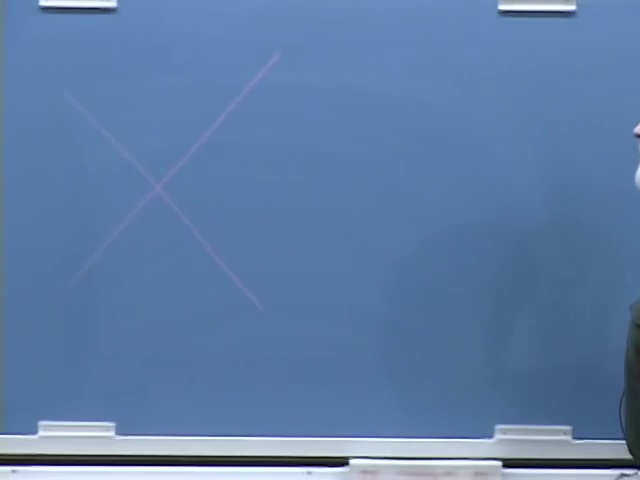
\includegraphics[width=0.68\textwidth]{lecture_09_figure_02.png}
\caption{Температура Хокинга \(T_H=1/(8\pi M)\) в естественных единицах.}
\lectureframe{00:08:12}
\end{figure}

Чем больше черная дыра, тем она холоднее. В лекции это объясняют, прослеживая назад типичный фотон. У тепловых фотонов характерная энергия \(E_\gamma\sim T_H\). Фотон, достигающий бесконечности с энергией порядка \(M^{-1}\), когда он возникает вблизи горизонта, имеет гораздо большую локальную энергию. Красное смещение между пригоризонтным слоем и бесконечностью сильнее для большей дыры, поэтому асимптотическая температура оказывается ниже.

\begin{classroomqa}
\audiencequestion{Если шварцшильдовское время замирает на горизонте, не следует ли нам прослеживать фотон, который изначально упал внутрь и увеличил массу дыры?\lecturetimestamp{00:04:19}}
\lecturerresponse{Для вопроса о температуре надо прослеживать фотоны, испускаемые наружу. Они начинаются с очень высокой локальной частоты, теряют энергию, выбираясь наружу, и приходят как излучение Хокинга. Судьба исходного падающего фотона — отдельный вопрос об информации.}
\end{classroomqa}

\section{Планковский слой и растянутый горизонт}

Насколько близко к горизонту можно доверять локальному соотношению из уравнения~\eqref{eq:l09-local-temperature}? В лекции планковская длина принимается за наименьшее осмысленное расстояние в полуклассическом описании. Это подсказывает наличие тонкого слоя примерно в одну планковскую длину снаружи от математического горизонта, заполненного флуктуациями планковского масштаба. Он непрерывно испускает и поглощает.

Большинство испущенных квантов не уходит. Лишь те, что направлены в очень узкий конус наружу, избегают падения обратно. Кванты, испущенные под произвольными углами, возвращаются к горизонту. Исходящие и входящие возбуждения сталкиваются, порождая пары и другие частицы; в этом смысле стационарное описание содержит тонкий слой чрезвычайно горячего вещества.

\begin{figure}[htbp]
\centering
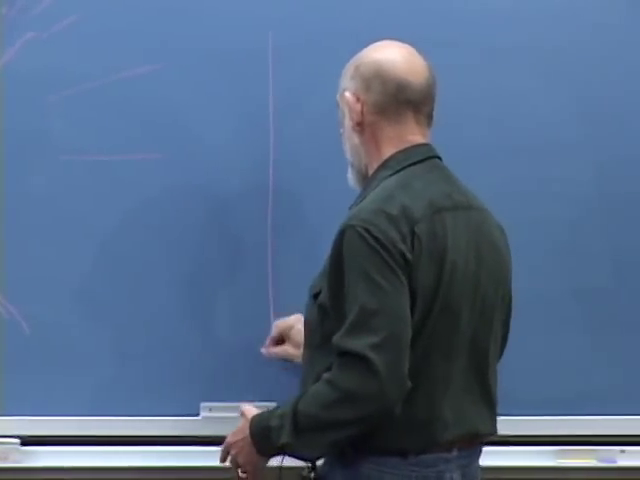
\includegraphics[width=0.74\textwidth]{lecture_09_figure_03.png}
\caption{Узкий конус выхода для пригоризонтного излучения. Большинство локально испущенных квантов возвращается к горизонту.}
\lectureframe{00:11:38}
\end{figure}

Существует и дополняющая пространственно-временная картина. Вдали от горизонта виртуальную флуктуацию можно схематически представить короткой замкнутой петлей: возбуждение частица–античастица возникает и исчезает прежде, чем оно сможет стать асимптотическим состоянием. Вблизи горизонта флуктуация может лежать по обе стороны причинной границы. Для внешнего наблюдателя внешняя часть выглядит как частица, испущенная горизонтом и позднее вновь поглощенная. Очень малая доля уходит и становится излучением Хокинга.

\begin{classroomqa}
\audiencequestion{На внешней диаграмме такая флуктуация простирается от \(t=-\infty\) до \(t=+\infty\)?\lecturetimestamp{00:15:00}}
\lecturerresponse{Точное классическое положение горизонта приводит к такому кажущемуся сингулярным описанию. На практике мы заменяем его растянутым горизонтом, времениподобной поверхностью примерно в одну планковскую длину снаружи. Тогда испускание и повторное поглощение происходят при конечных внешних временах.}
\end{classroomqa}

\begin{figure}[htbp]
\centering
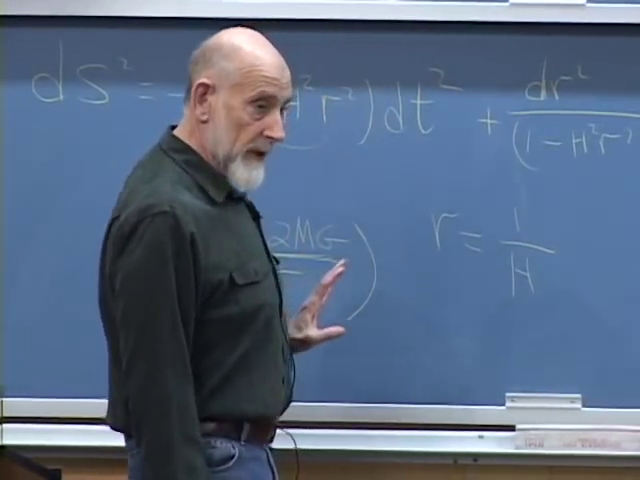
\includegraphics[width=0.72\textwidth]{lecture_09_figure_04.png}
\caption{Классический горизонт и расположенный рядом растянутый горизонт, используемый во внешнем описании.}
\lectureframe{00:15:52}
\end{figure}

Растянутый горизонт не является новой инвариантной границей. Это эффективная поверхность, помещаемая туда, где полуклассическая геометрия перестает быть надежной. Квантовые флуктуации материи и самой геометрии размывают точное положение на планковских масштабах. Эта конструкция сводит неопределенность к поверхности, на которой внешнее описание остается конечным.

В этом локальном рассуждении ничто не различает, принадлежит ли горизонт черной дыре или ускоренно расширяющейся Вселенной. Это и есть мост к пространству де Ситтера.

\section{Пространство де Ситтера в расширяющихся координатах}

Формальная лекция начинается с пространственно-плоского слоения пространства-времени де Ситтера,
\begin{equation}
ds^2=-dt^2+e^{2Ht}d\mathbf{x}^2,
\qquad
d\mathbf{x}^2=dx^2+dy^2+dz^2.
\label{eq:l09-flat-slicing}
\end{equation}
Константа \(H\) задает скорость расширения де Ситтера. Множитель появляется как \(e^{2Ht}\), потому что метрика измеряет квадрат расстояния; фиксированный координатный интервал имеет физическую длину
\begin{equation}
D(t)=e^{Ht}\lvert\Delta\mathbf{x}\rvert.
\end{equation}

\begin{figure}[htbp]
\centering
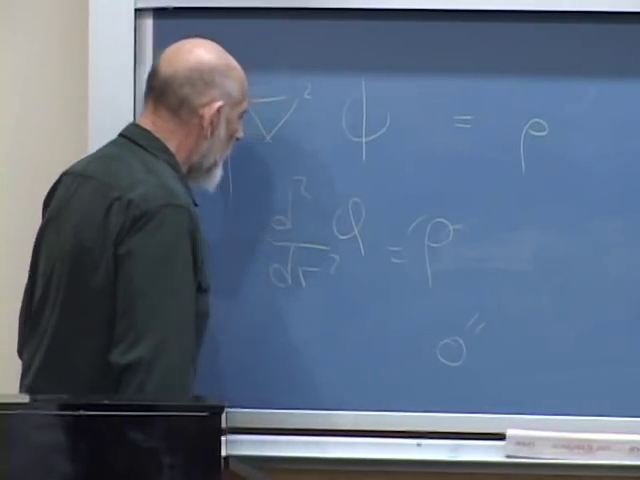
\includegraphics[width=0.78\textwidth]{lecture_09_figure_05.png}
\caption{Экспоненциально расширяющаяся метрика де Ситтера в плоских координатах.}
\lectureframe{00:18:50}
\end{figure}

Эти координаты наглядно показывают расширение, но помещают будущую бесконечность бесконечно далеко вверх по странице. Чтобы перенести ее на доску, введем конформное время
\begin{equation}
\eta=-\frac{1}{H}e^{-Ht},
\qquad
-\infty<\eta<0.
\label{eq:l09-conformal-time}
\end{equation}
Тогда
\begin{equation}
dt=\frac{d\eta}{-H\eta},
\qquad
e^{Ht}=-\frac{1}{H\eta},
\end{equation}
и уравнение~\eqref{eq:l09-flat-slicing} принимает вид
\begin{equation}
ds^2=\frac{1}{H^2\eta^2}
\left(-d\eta^2+d\mathbf{x}^2\right).
\label{eq:l09-conformal-metric}
\end{equation}
При \(t\to+\infty\) имеем \(\eta\to0^{-}\). Бесконечное собственное время сжато в конечную горизонтальную линию \(\eta=0\).

\editorialnote{Преобразование времени по ходу записи на доске несколько раз исправляется. Уравнение~\eqref{eq:l09-conformal-time} дает согласованную форму: раннее космическое время отображается в \(\eta\to-\infty\), а будущая бесконечность — в \(\eta\to0^{-}\).}

\begin{figure}[htbp]
\centering
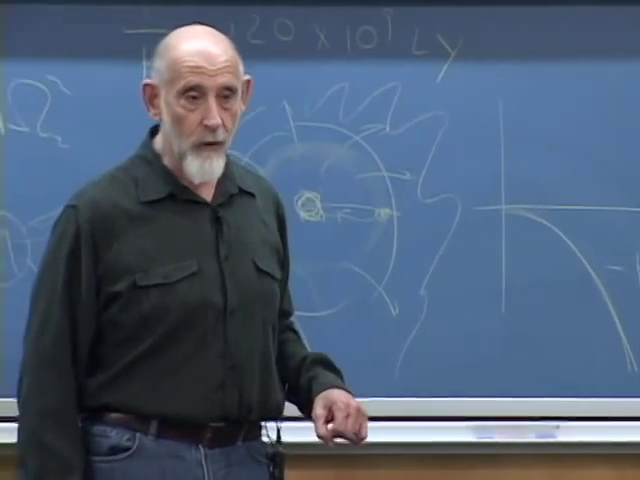
\includegraphics[width=0.82\textwidth]{lecture_09_figure_06.png}
\caption{Преобразование к конформному времени и конформно-плоская метрика.}
\lectureframe{00:21:24}
\end{figure}

Конформный множитель умножает и временной, и пространственный члены, поэтому не изменяет светоподобные направления. Для радиального светового луча,
\begin{equation}
ds^2=0
\quad\Longrightarrow\quad
-d\eta^2+dx^2=0
\quad\Longrightarrow\quad
\frac{dx}{d\eta}=\pm1.
\label{eq:l09-null-rays}
\end{equation}
Следовательно, на конформной диаграмме свет идет под углом \(45^\circ\). Поэтому смена координат полезна: причинная достижимость становится видимой.

\section{Причинная область одного наблюдателя}

Представьте наблюдателя, мировая линия которого продолжается в течение бесконечного собственного времени. На компактифицированной диаграмме она оканчивается в одной точке на \(\eta=0\). Любой сигнал, который он вообще может получить, лежит внутри обратного светового конуса этой конечной точки. События вне этого конуса никогда не могут послать ему сигнал, сколько бы он ни ждал.

\begin{figure}[htbp]
\centering
\includegraphics[width=0.78\textwidth]{lecture_09_figure_07.png}
\caption{Предельный обратный световой конус наблюдателя в конформных координатах де Ситтера.}
\lectureframe{00:24:38}
\end{figure}

У второго наблюдателя другой конус. Эти две доступные области перекрываются, но ни одна не охватывает все пространство-время. В дальнейшем мы примем точку зрения первого и будем называть этот обратный световой конус каузальной областью наблюдателя.

На рисунке кажется, будто область сжимается по направлению к будущему, но координатная ширина не есть собственное расстояние. На срезе при постоянном \(\eta\) квадрат физического расстояния между наблюдателем в точке \(x=0\) и горизонтом в точке \(x=\Delta x\) равен
\begin{equation}
D^2=\frac{(\Delta x)^2}{H^2\eta^2}.
\label{eq:l09-horizon-distance-start}
\end{equation}
Горизонт — нулевая линия под углом \(45^\circ\), оканчивающаяся при \(\eta=0\), поэтому
\begin{equation}
\Delta x=\lvert\eta\rvert.
\end{equation}
Подстановка дает
\begin{equation}
D_{\rm hor}^2=\frac{1}{H^2},
\qquad
D_{\rm hor}=\frac{1}{H}.
\label{eq:l09-horizon-radius}
\end{equation}
Координатное расстояние уменьшается, но конформный множитель растет ровно настолько, чтобы это скомпенсировать. Собственный радиус горизонта постоянен.

\begin{figure}[htbp]
\centering
\includegraphics[width=0.80\textwidth]{lecture_09_figure_08.png}
\caption{Вывод на доске, переводящий сжимающийся координатный интервал в фиксированное собственное расстояние \(H^{-1}\).}
\lectureframe{00:28:42}
\end{figure}

\section{Статическая область}

Постоянный радиус горизонта подсказывает координаты, приспособленные к центральному наблюдателю. Не выводя преобразование координат, в лекции записывают результат:
\begin{equation}
ds^2=
-\left(1-H^2r^2\right)d\tau^2
+\frac{dr^2}{1-H^2r^2}
+r^2d\Omega_2^2.
\label{eq:l09-static-patch}
\end{equation}
Коэффициенты зависят от \(r\), а не от \(\tau\). Эта координатная карта покрывает статическую область наблюдателя,
\begin{equation}
0\le r<\frac{1}{H}.
\end{equation}

\begin{figure}[htbp]
\centering
\includegraphics[width=0.88\textwidth]{lecture_09_figure_09.png}
\caption{Метрика статической области де Ситтера и ее сравнение с фактором Шварцшильда.}
\lectureframe{00:34:22}
\end{figure}

Сходство со Шварцшильдом видно сразу:
\begin{equation}
f_{\rm dS}(r)=1-H^2r^2,
\qquad
f_{\rm Schw}(r)=1-\frac{2G_NM}{r}.
\end{equation}
В обоих случаях горизонт в статических координатах находится там, где \(f(r)=0\). Для де Ситтера
\begin{equation}
1-H^2r^2=0
\quad\Longrightarrow\quad
r_H=H^{-1}.
\end{equation}
Здесь карта сингулярна, точно так же как координаты Шварцшильда сингулярны на горизонте черной дыры. Тем не менее глобальные геометрии различаются важным образом. Наблюдатель у черной дыры находится снаружи и смотрит внутрь; наблюдатель де Ситтера находится внутри и смотрит наружу.

\begin{classroomqa}
\audiencequestion{Как геометрия может быть статической, если свободно отпущенные частицы расходятся в экспоненциально расширяющейся Вселенной?\lecturetimestamp{00:36:06}}
\lecturerresponse{Статичность не означает, что каждая частица остается неподвижной. Это означает, что коэффициенты метрики и результат повторного эксперимента не зависят от момента начала. Отпустите сейчас две частицы — и они начнут ускоренно расходиться; повторите тот же эксперимент позже — и произойдет то же самое движение.}
\end{classroomqa}

\begin{classroomqa}
\audiencequestion{Наблюдают ли две расходящиеся частицы красное смещение друг друга?\lecturetimestamp{00:38:34}}
\lecturerresponse{Да. Их возрастающее разделение вызывает относительное красное смещение, хотя метрика, приспособленная к наблюдателю, не зависит от времени.}
\end{classroomqa}

\section{Температура, наблюдаемая изнутри}

Пригоризонтные структуры пространства Шварцшильда и де-ситтеровского пространства локально эквивалентны. Поэтому горизонт де Ситтера испускает и вновь поглощает тепловые кванты. Редкий фотон распространяется внутрь, к центральному наблюдателю, теряя энергию при подъеме по потенциалу статической области. Измеряемая в центре температура Гиббонса--Хокинга равна
\begin{equation}
T_{\rm dS}=\frac{H}{2\pi}
\label{eq:l09-de-sitter-temperature}
\end{equation}
в естественных единицах. Неподвижный термометр на радиусе \(r\) показывает значение с толмановским красным смещением
\begin{equation}
T_{\rm local}(r)=
\frac{T_{\rm dS}}{\sqrt{1-H^2r^2}},
\label{eq:l09-tolman}
\end{equation}
которое расходится при \(r\to H^{-1}\) и вблизи горизонта сводится к уравнению~\eqref{eq:l09-local-temperature}.

\editorialnote{В лекции масштаб получают из расстояния до горизонта и красного смещения, а не выписывают явно уравнения~\eqref{eq:l09-de-sitter-temperature} и \eqref{eq:l09-tolman}. Здесь указана стандартная нормировка этого рассуждения.}

Для наблюдаемого позднего ускорения в лекции используется оценка периода
\begin{equation}
H^{-1}\sim 20\times10^9\ {\rm light\ years}.
\label{eq:l09-lecture-horizon-estimate}
\end{equation}
Тогда типичный фотон горизонта имеет длину волны, сравнимую с миллиардами световых лет. Это не реликтовое микроволновое излучение; оно несравненно холоднее.

Операциональный мысленный эксперимент — это удочка космологического масштаба. Алиса остается при \(r=0\), прикрепляет термометр к очень длинному тросу, по которому также передаются данные, и позволяет космическому отталкиванию унести прибор наружу. Она останавливает его чуть не доходя до горизонта, ждет возвращения сигнала и обнаруживает большую локальную температуру. Термометр рядом с ней в центре показывает крошечное значение \(H/(2\pi)\). Один и тот же горизонт допускает оба показания, потому что они снимаются при разных гравитационных потенциалах.

\section{Пересечение горизонта}

Классическое внешнее описание напоминает знакомую историю с черной дырой. Боб в центре наблюдает, как Алиса удаляется. Ее сигналы испытывают все большее красное смещение и приходят все медленнее; она кажется распластанной по горизонту и в конце концов гаснет. Более поздняя путешественница, Джейн, выглядит как еще один, более тонкий слой в осадочной стопке у границы.

\begin{classroomqa}
\audiencequestion{С нашей точки зрения, проходят ли объекты вообще через космологический горизонт?\lecturetimestamp{00:45:30}}
\lecturerresponse{Не в классическом описании статического наблюдателя. Их сигналы краснеют и затухают, тогда как их видимое положение приближается к горизонту. Однако в их собственном свободнопадающем описании они пересекают его, не встречая локально сингулярной поверхности.}
\end{classroomqa}

\begin{classroomqa}
\audiencequestion{Горизонт горяч только для наблюдателей, которые остаются поблизости, не пересекая его? Падающий наблюдатель ведь не поджаривается просто от того, что проходит через него, верно?\lecturetimestamp{00:48:27}}
\lecturerresponse{В своей системе отсчета Алиса пересекает его гладко. Экстремальная температура относится к стационарному описанию. Если Боб настаивает на том, чтобы разрешать Алису все ближе к горизонту, ему приходится облучать ее все более короткими длинами волн. Такая попытка построить гейзенберговский микроскоп тогда вносит достаточно энергии, чтобы поджарить то, что он пытается наблюдать.}
\end{classroomqa}

Это не противоречие между двумя локальными событиями. Стационарный наблюдатель и падающий используют радикально разные измерения. Комплементарность горизонта ставит вопрос о том, как оба описания могут быть верны, не позволяя одному наблюдателю напрямую сравнить дублированную информацию.

\section{Ньютоновская модель отталкивания вакуума}

В этот момент студент спрашивает, что заменяет гравитационный колодец черной дыры. Сасскинд отвечает, строя ньютоновскую модель. Пусть \(\phi\) — гравитационный потенциал, так что ускорение пробной частицы равно
\begin{equation}
\mathbf{a}=-\boldsymbol{\nabla}\phi.
\end{equation}
Для обычного нерелятивистского вещества уравнение Пуассона имеет вид
\begin{equation}
\nabla^2\phi=4\pi G_N\rho.
\label{eq:l09-poisson}
\end{equation}

\begin{classroomqa}
\audiencequestion{Если эффекты черной дыры связаны с ее гравитационным колодцем, что служит соответствующим источником в пространстве де Ситтера?\lecturetimestamp{00:49:36}}
\lecturerresponse{Сама энергия вакуума дает пространственно однородный гравитационный источник. В ньютоновском описании она создает квадратичный потенциал, а не колодец вида \(1/r\).}
\end{classroomqa}

\begin{figure}[htbp]
\centering
\includegraphics[width=0.78\textwidth]{lecture_09_figure_10.png}
\caption{Уравнение Пуассона и схематическая радиальная форма второй производной, используемая в лекции.}
\lectureframe{00:51:38}
\end{figure}

На доске опускаются нормировка, члены сферической меры, давление и поначалу даже общий знак, так что упражнение сводится к
\begin{equation}
\frac{d^2\phi}{dr^2}\sim H^2.
\end{equation}
Существенный вывод состоит в том, что постоянный источник дает квадратичную функцию. При знаке, требуемом отталкиванием де Ситтера,
\begin{equation}
\phi_{\rm dS}(r)=-\frac{1}{2}H^2r^2,
\qquad
a_r=-\frac{d\phi_{\rm dS}}{dr}=H^2r.
\label{eq:l09-de-sitter-potential}
\end{equation}
Ускорение направлено наружу и растет линейно с расстоянием. Решение уравнения \(\ddot r=H^2r\) дает
\begin{equation}
r(\tau)=A e^{H\tau}+B e^{-H\tau},
\end{equation}
так что растущая ветвь воспроизводит экспоненциальное расхождение.

\begin{figure}[htbp]
\centering
\includegraphics[width=0.76\textwidth]{lecture_09_figure_11.png}
\caption{Уравнение для однородного источника и квадратичный потенциал де Ситтера.}
\lectureframe{00:53:32}
\end{figure}

\editorialnote{В общей теории относительности слабополевое ускорение однородной жидкости зависит от \(\rho+3p\), а не только от \(\rho\). Для вакуумной энергии \(p=-\rho\), так что \(\rho+3p=-2\rho\) и ускорение является отталкивающим. Уравнение~\eqref{eq:l09-de-sitter-potential} дает правильно нормированный результат де Ситтера; вычисление на доске намеренно отслеживает только квадратичную зависимость и знак.}

Поместим в центр обычную массу \(M\). Тогда качественный потенциал принимает вид
\begin{equation}
\phi(r)=-\frac{G_NM}{r}-\frac{1}{2}H^2r^2,
\label{eq:l09-combined-potential}
\end{equation}
а радиальное ускорение равно
\begin{equation}
a_r=-\frac{G_NM}{r^2}+H^2r.
\end{equation}
При малых \(r\) побеждает локальное притяжение; при больших \(r\) побеждает вакуумное отталкивание. Их баланс достигается при
\begin{equation}
r_\ast=\left(\frac{G_NM}{H^2}\right)^{1/3}.
\label{eq:l09-turnaround}
\end{equation}
Это аккуратная версия максимума потенциала из лекции. Это качественно объясняет, почему близкие гравитационно связанные системы могут оставаться связанными, тогда как достаточно далекие галактики ускоренно удаляются.

\begin{figure}[htbp]
\centering
\includegraphics[width=0.78\textwidth]{lecture_09_figure_12.png}
\caption{Обычное притяжение вида \(1/r\) в сочетании с перевернутым квадратичным потенциалом де Ситтера.}
\lectureframe{00:58:20}
\end{figure}

\begin{classroomqa}
\audiencequestion{Обычные силы по-прежнему важны, или вакуумное отталкивание в конце концов разрывает всякий остров материи?\lecturetimestamp{00:57:29}}
\lecturerresponse{Нужно учитывать все силы. На достаточно малых масштабах доминируют электромагнитное связывание и локальная гравитация. Вакуумное отталкивание становится существенным лишь на огромных расстояниях, задаваемых \(H^{-1}\) и масштабом равновесия, соответствующим данной связанной массе.}
\end{classroomqa}

\section{Один источник, несколько названий}

Теперь ненадолго остановимся на терминологии. В используемой модели энергия вакуума, космологическая постоянная и тёмная энергия — не три аддитивные субстанции. Это три описания одного и того же источника \(w=-1\). Можно говорить о постоянном члене в уравнении Эйнштейна, о лоренц-инвариантной плотности энергии вакуума или о компоненте, вызывающей ускорение на поздних временах.

\begin{classroomqa}
\audiencequestion{Присутствуют ли однородный ньютоновский источник и квантовая энергия вакуума одновременно как отдельные эффекты?\lecturetimestamp{00:59:14}}
\lecturerresponse{Нет. Однородная плотность — это ньютоновская модель того же самого источника. Энергия вакуума, космологическая постоянная и, в этой лекции, тёмная энергия обозначают одну физическую компоненту.}
\end{classroomqa}

\begin{classroomqa}
\audiencequestion{Имеет ли тогда одно и то же явление классическое описание и квантовое описание?\lecturetimestamp{01:00:32}}
\lecturerresponse{Его микроскопическое происхождение может быть квантово-механическим, подобно тому как часть массы электрона имеет квантовое происхождение. Как только эффективная плотность энергии известна, она входит в классические гравитационные уравнения как обычный источник. Окончательного происхождения наблюдаемого значения мы не знаем.}
\end{classroomqa}

В планковских единицах наблюдаемая плотность энергии вакуума чрезвычайно мала:
\begin{equation}
\rho_\Lambda\sim10^{-123}\rho_{\rm Pl},
\label{eq:l09-planck-smallness}
\end{equation}
с точностью до соглашения, используемого для планковской плотности. Именно это малое число и составляет проблему космологической постоянной. По той же причине горизонт так велик: в четырёх измерениях
\begin{equation}
H^2=\frac{8\pi G_N}{3}\rho_\Lambda,
\qquad
r_H=H^{-1}.
\end{equation}
Если бы \(H\) было больше, горизонт был бы меньше, температура де Ситтера в центре — выше, а отталкивающее ускорение \(H^2r\) — сильнее.

\begin{classroomqa}
\audiencequestion{Связана ли крошечная космологическая постоянная с постоянной Планка и квантовыми флуктуациями?\lecturetimestamp{01:03:27}}
\lecturerresponse{Наиболее ясное сравнение получается в безразмерных планковских единицах, где \(G_N=\hbar=c=1\). В этих единицах плотность вакуума примерно на \(123\) порядков величины меньше естественной планковской плотности. Объяснение этой иерархии — одна из центральных загадок фундаментальной физики.}
\end{classroomqa}

\begin{classroomqa}
\audiencequestion{Должна ли энергия вакуума быть в точности постоянной космологической постоянной? Может ли ускоряющая компонента уменьшаться и в конце концов установиться на нуле?\lecturetimestamp{01:04:52}}
\lecturerresponse{Это логически возможная альтернатива: динамическое поле тёмной энергии могло бы изменяться со временем. В лекции принимается случай постоянной не потому, что все альтернативы были доказаны невозможными, а потому, что доступные на тот момент наблюдения всё сильнее указывали на поведение, близкое к космологической постоянной.}
\end{classroomqa}

\section{Астрономия в далёком будущем}

В асимптотически де-ситтеровской вселенной структуры, не связанные гравитационно, в конце концов пересекают горизонт наблюдателя. Космическое микроволновое фоновое излучение из-за красного смещения уходит ниже порога обнаружения. Далёкие галактики исчезают. Уцелевший астроном может видеть лишь слившийся локальный гравитационный остров внутри в остальном тёмной области.

\begin{classroomqa}
\audiencequestion{Без телескопа кто-нибудь вообще заметил бы, что далёкие галактики исчезли?\lecturetimestamp{01:06:17}}
\lecturerresponse{Вероятно, нет. Серьёзная проблема глубже: даже при наличии развитых приборов у будущих наблюдателей может не оказаться далёких трассеров и микроволнового фона, по которым мы сегодня делаем вывод о расширении.}
\end{classroomqa}

Тогда старая картина «островной вселенной» могла бы показаться убедительной. Парадокс Ольберса не заставил бы прийти к иному выводу, потому что он предполагает бесконечную, статическую, однородную совокупность светящихся источников; будущий наблюдатель видел бы лишь конечное число звёзд локального острова. Тёмная энергия не создаёт непрерывно новые галактики из пустого пространства взамен исчезнувших.

В точном пространстве де Ситтера горизонт не сжимается вокруг локальной галактики. Его физический радиус остаётся равным \(H^{-1}\), что неизмеримо больше размера галактики. Исчезает же несвязанная материя, уносимая за эту фиксированную причинную границу.

\begin{classroomqa}
\audiencequestion{Могли бы звёзды, выброшенные из галактики, служить пробными телами для обнаружения крупномасштабной геометрии?\lecturetimestamp{01:11:25}}
\lecturerresponse{Некоторое время — да. Выброшенные объекты и световые сигналы на больших базах могли бы зондировать геометрию. Но эффект становится заметным лишь на расстояниях порядка значительной доли миллиарда световых лет, так что эксперимент занял бы космологическое время.}
\end{classroomqa}

\begin{classroomqa}
\audiencequestion{Откуда мы знаем, что далёкий горизонт уже не скрыл от нас большую часть вселенной?\lecturetimestamp{01:11:45}}
\lecturerresponse{Мы уже видим достаточно много галактик, красных смещений и фонового излучения, чтобы измерить расширение и восстановить крупномасштабную геометрию. Будущие наблюдатели, лишённые этих трассеров, столкнулись бы с намного более трудной задачей вывода.}
\end{classroomqa}

\begin{classroomqa}
\audiencequestion{Если бы горизонт лежал сразу за Андромедой, было бы его присутствие очевидно?\lecturetimestamp{01:12:19}}
\lecturerresponse{Да. Такой маленький горизонт потребовал бы гораздо большего \(H\), и возникающее отталкивание сильно изменило бы движение Андромеды. Измеренное значение, напротив, помещает асимптотический горизонт на несравненно больший масштаб.}
\end{classroomqa}

\begin{classroomqa}
\audiencequestion{Могут ли за нашим горизонтом происходить новые Большие взрывы?\lecturetimestamp{01:13:25}}
\lecturerresponse{События за горизонтом не видны ни нам, ни нашим потомкам. Родственная, но более точная возможность — нуклеация пузырей при вечной инфляции — будет рассмотрена позже в лекции.}
\end{classroomqa}

Имея ракеты, часы и несколько миллиардов лет, будущие наблюдатели могли бы отправить исследователей через значительную часть этой области и восстановить её метрику. Однако на обычных лабораторных или цивилизационных масштабах времени этот эффект почти недоступен. Это различие поправляет слишком сильное утверждение, будто расширение было бы невозможно обнаружить: оно операционально труднодоступно, а не запрещено в принципе.

\begin{classroomqa}
\audiencequestion{Могли бы будущие исследователи определить геометрию гораздо раньше, не дожидаясь теплового возврата?\lecturetimestamp{01:21:40}}
\lecturerresponse{Безусловно. Возврат не является предлагаемым измерением. Исследователи, обмениваясь световыми сигналами на базах в миллиарды световых лет, могли бы построить карту статического патча за несравненно более короткое, хотя всё же космологическое, время.}
\end{classroomqa}

\begin{classroomqa}
\audiencequestion{Стерло бы красное смещение всю информацию, возвращённую такими исследователями?\lecturetimestamp{01:23:24}}
\lecturerresponse{Нет, если они зондируют масштабы, лежащие далеко внутри горизонта. База порядка миллиарда световых лет уже чувствительна к расширению и при этом даёт лишь умеренное красное смещение. Эксперимент ограничен главным образом своей огромной длительностью.}
\end{classroomqa}

\section{Конечная энтропия и возврат}

В термодинамическом смысле статический патч не пуст. Его горизонт характеризуется площадью
\begin{equation}
A_H=4\pi H^{-2},
\end{equation}
температурой \(T_{\rm dS}=H/(2\pi)\) и энтропией
\begin{equation}
S_{\rm dS}=\frac{A_H}{4G_N}
=\frac{\pi}{G_NH^2}
\label{eq:l09-de-sitter-entropy}
\end{equation}
в единицах \(\hbar=c=k_B=1\). Энтропия конечна. Поэтому статический патч, с должной осторожностью, можно представлять как тепловую полость с конечной энтропией, возбуждения которой в стационарном описании сосредоточены вблизи горизонта.

Обычный ящик с газом в равновесии на коротких временах кажется лишённым особенностей, но статистическая механика не запрещает флуктуаций. Если макросостояние имеет дефицит энтропии \(\Delta S\) по сравнению с равновесием, его вероятность примерно равна
\begin{equation}
P\sim e^{-\Delta S}.
\label{eq:l09-fluctuation-probability}
\end{equation}
Соответствующее время ожидания растёт как
\begin{equation}
t\sim t_0 e^{\Delta S}.
\end{equation}
Для конечной системы время возвращения в состояние, сколь угодно близкое к более раннему, есть время возврата Пуанкаре,
\begin{equation}
t_{\rm rec}\sim H^{-1}e^{S_{\rm dS}}.
\label{eq:l09-recurrence}
\end{equation}
Поскольку \(S_{\rm dS}\) для нашего горизонта имеет порядок \(10^{120}\), в лекции этот масштаб кратко записывается как \(e^{10^{120}}\). Измеряется ли префактор в годах, хаббловских временах или микроскопических единицах, это несущественно по сравнению с двойной экспонентой.

\begin{figure}[htbp]
\centering
\includegraphics[width=0.76\textwidth]{lecture_09_figure_13.png}
\caption{Обсуждение возврата; на доске — огромный экспоненциальный масштаб времени ожидания.}
\lectureframe{01:16:24}
\end{figure}

До такого возврата меньшие флуктуации встречаются несравненно чаще. Все молекулы в комнате могли бы собраться в одном углу; мог бы ненадолго образоваться сложный вихрь; в шутливой иерархии лекции тепловое движение могло бы собрать слона. Чем меньше требуемый дефицит энтропии, тем дешевле флуктуация.

\begin{classroomqa}
\audiencequestion{Являются ли возвраты Пуанкаре именно следствием квантовой механики?\lecturetimestamp{01:25:44}}
\lecturerresponse{Нет. Возвраты и редкие флуктуации возникают уже в классической статистической механике. Их применение к пространству де Ситтера использует нашу нынешнюю физическую картину, которая когда-нибудь может быть пересмотрена, но термодинамика и статистические рассуждения — одни из самых надёжных известных нам структур.}
\end{classroomqa}

Само значение вероятности в будущей теории может обрести более глубокий смысл. Susskind этого не отрицает. Его более узкий тезис состоит в том, что отказ от статистической механики лишь потому, что ее следствия на больших временах странны, означал бы отбросить один из лучше всего проверенных структурирующих принципов физики.

\section{Мозги Больцмана и типичные наблюдатели}

Предположим, что тепловая флуктуация создает целое состояние, подобное Большому взрыву. Это требует огромного уменьшения энтропии. Флуктуация, создающая одну солнечную систему, менее затратна; уже теплая Земля обходится еще дешевле. Если требуется лишь один наблюдатель, то наименее затратная флуктуация могла бы создать только функционирующий мозг с кажущимися воспоминаниями. Такого гипотетического наблюдателя называют мозгом Больцмана.

Проблема не в том, логически ли возможна одна странная флуктуация. Проблема в том, предсказывает ли космологическая модель, что почти каждый наблюдатель является именно такой флуктуацией. Мы рассуждаем, исходя из наших наблюдений, предполагая, что не являемся фантастически нетипичными. Теория, в которой обычные наблюдатели со связными космическими историями экспоненциально уступают по численности изолированным тепловым мозгам, подрывает такой вывод.

Поэтому проблема мозгов Больцмана — это количественная проверка на согласованность. Сравнивают ожидаемую численность обычных наблюдателей с численностью наблюдателей, порожденных флуктуациями. Если преобладают последние, то либо вакуум должен распасться прежде, чем они начнут возникать в огромном количестве, либо нужно изменить меру, либо следует пересмотреть космологические предположения.

Более ранний вопрос об ультрафиолетово--инфракрасной связи здесь явно откладывается. Аргумент о рекуррентности не зависит от разрешения этого отдельного вопроса.

\section{Вечная инфляция и пузырьковые вселенные}

Далее в лекции, не пытаясь дать полный вывод, вводится вторая вероятностная проблема. В метастабильном вакууме де Ситтера может нуклеироваться пузырь, в котором энергия вакуума ниже. Стенка пузыря расширяется, а его внутренняя область может развиться в открытую вселенную Фридмана--Робертсона--Уокера. Тем временем окружающая инфлирующая область продолжает расширяться и нуклеирует новые пузыри.

\begin{figure}[htbp]
\centering
\includegraphics[width=0.74\textwidth]{lecture_09_figure_14.png}
\caption{Пузырь с меньшей энергией вакуума, изображенный внутри инфлирующего фона де Ситтера.}
\lectureframe{01:29:38}
\end{figure}

Ключевая особенность состоит в экспоненциальном росте числа областей. Новый физический объем возникает быстрее, чем его поглощают пузыри, так что число пузырьковых областей растет без границ. Разные пузыри могут перейти в разные низкоэнергетические состояния и потому проявлять разную эффективную физику.

Чтобы выявить статистическую трудность, Susskind сначала отходит от космологии и рассматривает экспоненциально растущую человеческую популяцию с конечными, но неизвестными ресурсами. Предположим, что наблюдатели типичны среди всех людей за все время существования популяции. Если население удваивается в каждом поколении, а затем заканчивается, то половина всех людей живет в последнем поколении, три четверти — в двух последних, а семь восьмых — в трех последних:
\begin{equation}
f_n=1-2^{-n}.
\label{eq:l09-last-generations}
\end{equation}
Тогда предположение о типичности помещало бы нас неприятно близко к концу, хотя об общем запасе ресурсов нам ничего не известно. Это предлагается не как надежное предсказание вымирания человечества. Это предупреждение о том, что при экспоненциальном росте результат подсчета определяется отсечкой.

Пример с подбрасыванием монеты яснее формулирует обычное предположение о типичности. Если много экспериментаторов каждый подбрасывает честную монету \(N\) раз, то подавляющее большинство получает
\begin{equation}
n_H=\frac{N}{2}+O(\sqrt{N}).
\end{equation}
Наблюдатель с экстремальным результатом должен прежде всего заподозрить плохую модель или плохую монету, а не без доказательств считать, что он находится в фантастически редком хвосте распределения. Космологическая вероятность опирается на то же интуитивное представление о типичности, но в бесконечной популяции ей нужен четко определенный способ подсчета.

\section{Граница Эшера и проблема меры}

Геометрическая аналогия Susskind — это работа M.\ C.\ Escher \emph{Circle Limit IV}, диск, замощенный ангелами и дьяволами, которые кажутся меньше по мере приближения к границе. В гиперболической геометрии, представленной на рисунке, эти фигуры эквивалентны; их кажущийся евклидов размер меняется только из-за проекции.

\begin{figure}[htbp]
\centering
\includegraphics[width=0.76\textwidth]{lecture_09_figure_15.png}
\caption{Нарисованный на доске суррогат экспоненциально размножающихся фигур Эшера у круговой границы.}
\lectureframe{01:37:54}
\end{figure}

Представьте, что у Эшера конечны время, чернила и терпение. У края он в конце концов останавливается, возможно оставляя некоторые фигуры незавершенными. Поскольку число фигур экспоненциально растет с гиперболическим радиусом, конечный внешний слой содержит фиксированную по порядку величины долю всех нарисованных фигур. Приблизительно половина может лежать в последнем слое, как бы далеко наружу ни сдвигали отсечку.

Теперь спросим об отношении числа ангелов к числу дьяволов. В идеальном бесконечном узоре симметрия подсказывает равенство один к одному. Однако при любом конечном подсчете немного иная граница может включить гораздо больше фигур одного типа. Поскольку большая часть подсчета сосредоточена у границы, малая деформация этой границы приводит к изменению ответа на величину порядка единицы.

\begin{figure}[htbp]
\centering
\includegraphics[width=0.76\textwidth]{lecture_09_figure_16.png}
\caption{Граница отсечки доминирует в подсчете в экспоненциально растущем узоре.}
\lectureframe{01:43:06}
\end{figure}

Та же неоднозначность возникает и в вечной инфляции. Подсчитайте синие и розовые пузырьковые вселенные до некоторой временной отсечки, а затем сдвиньте отсечку на более позднее время. Оба подсчета расходятся, и их отношение может чувствительно зависеть от того, что понимается под \emph{time} и как проведена поверхность отсечки. Вероятностная мера — это предписание, которое регуляризует бесконечную популяцию и извлекает относительные вероятности. То, что разные правдоподобные предписания не согласуются друг с другом, и есть проблема меры.

\begin{classroomqa}
\audiencequestion{Есть ли связь между этой проблемой отсечки и ренормализацией?\lecturetimestamp{01:45:43}}
\lecturerresponse{Есть аналогия. В квантовой теории поля вводят решетку или ультрафиолетовую отсечку, затем уточняют ее и ищут величины, нечувствительные к краевым деталям регуляризатора. Космологи надеются на столь же устойчивое извлечение относительных вероятностей из вечной инфляции, но в обсуждаемой здесь схеме пока нет столь же решающего предписания.}
\end{classroomqa}

Эту аналогию не следует преувеличивать. Ренормализация успешна, когда контролируемый поток выделяет наблюдаемые, не зависящие от регуляризатора. Проблема меры как раз и состоит в том, что аналогичные инвариантные вопросы и предельная процедура остаются неясными. Сказать, что, возможно, мы задаем неправильный вопрос, — не решение, пока не указан правильный.

\begin{classroomqa}
\audiencequestion{Является ли эта картина с пузырями тем же самым явлением, что и инфляция в ранней Вселенной?\lecturetimestamp{01:48:19}}
\lecturerresponse{Они тесно связаны. При вечной инфляции родительский фон продолжает инфлировать, в то время как внутренние области локальных пузырей проходят собственную космологическую эволюцию. Наша наблюдаемая Вселенная могла бы находиться внутри одной такой области.}
\end{classroomqa}

\section{Можно ли увидеть столкновения пузырей?}

При встрече двух пузырей их энергии вакуума не просто складываются. Области с разными вакуумными состояниями разделяет доменная стенка, и геометрия этой стенки определяет, что может наблюдать каждая из сторон. В зависимости от положения столкновения относительно нашего прошлого светового конуса его след может быть скрыт или видим.

\begin{classroomqa}
\audiencequestion{Что происходит при столкновении двух вакуумных пузырей?\lecturetimestamp{01:52:07}}
\lecturerresponse{Столкновение создает геометрию доменной стенки, поведение которой зависит от двух вакуумов и от натяжения стенки. При благоприятных причинных обстоятельствах возмущение может войти в нашу наблюдаемую область и оставить анизотропный след.}
\end{classroomqa}

В лекции обсуждается холодная область в космическом микроволновом фоне как возможный кандидат и указывается на поляризацию вокруг круговой особенности как на различающий признак. Это намеренно подается как возможность, а не как обнаружение. Убедительный сигнал столкновения был бы революционным, потому что дал бы прямое свидетельство в пользу существования соседних пузырьковых областей и сделал бы проблему меры экспериментально неотложной.

\begin{figure}[htbp]
\centering
\includegraphics[width=0.70\textwidth]{lecture_09_figure_17.png}
\caption{Круговая особенность на небе и ее возможная картина поляризации в обсуждении столкновений пузырей.}
\lectureframe{01:50:22}
\end{figure}

\editorialnote{Обсуждение холодного пятна фиксирует состояние наблюдательных данных и предложения на момент лекции. Сама по себе температурная аномалия не является свидетельством столкновения пузырей; потребовался бы детальный, коррелированный сигнал.}

\begin{classroomqa}
\audiencequestion{Являются ли пузыри четырехмерными и какова пространственная кривизна их внутренних областей?\lecturetimestamp{01:53:37}}
\lecturerresponse{Это области пространства-времени, а не трехмерные мыльные пузыри, эволюционирующие во внешнем времени. Их внутренние области, как правило, представляют собой открытые вселенные FRW с отрицательной пространственной кривизной. Столкновение возмущает эту геометрию, но не просто превращает отрицательную кривизну в положительную.}
\end{classroomqa}

\section{Что теория струн устанавливает, а чего не устанавливает}

Заключительное обсуждение начинается с предложения приписать вероятность тому, что теория струн верна. Susskind отказывается назвать число, потому что само утверждение слишком неоднозначно. Вместо этого он разделяет два утверждения.

Во-первых, существует жёстко ограниченная математическая структура, сочетающая квантовую механику и гравитацию. Она дала точные результаты и глубокие математические тождества, а её внутренняя согласованность выдержала очень тщательную проверку. В неформальной терминологии лекции это \emph{String Theory} с заглавной \(S\). Наиболее хорошо понятые версии в значительной мере опираются на суперсимметрию.

Во-вторых, наблюдаемый мир не суперсимметричен при доступных энергиях. Чтобы связать точные суперсимметричные конструкции с нашей несуперсимметричной Вселенной, нужны нарушение суперсимметрии и более широкая структура, которая не поддаётся контролю с той же точностью. В терминологии лекции это предполагаемое расширение — \emph{string theory} с маленькой \(s\).

\begin{classroomqa}
\audiencequestion{Можно ли приписать вероятность тому, что теория струн является правильной теорией природы?\lecturetimestamp{01:54:18}}
\lecturerresponse{Нельзя делать это ответственно, не уточнив, какое именно утверждение имеется в виду. Точные математические структуры существуют и включают квантовую гравитацию, но строго контролируемые суперсимметричные модели не являются буквально нашим наблюдаемым миром. По вопросу о том, содержит ли более широкое расширение наш мир, у физиков могут быть обоснованные предварительные мнения; говорить же о чётко определённой численной вероятности нельзя.}
\end{classroomqa}

Аналогия — с механикой до появления полного математического аппарата. Можно было знать \(F=ma\) и закон силы обратных квадратов, но уметь решать только высокосимметричные круговые орбиты. Этот решаемый сектор был бы подлинным, но не исчерпывал бы всей теории. Точно так же точные суперсимметричные струнные конструкции могут быть особой, необычно удобной для анализа областью более широкой структуры.

\begin{figure}[htbp]
\centering
\includegraphics[width=0.60\textwidth]{lecture_09_figure_18.png}
\caption{Вложенная картина лекции: строго контролируемые суперсимметричные струнные конструкции внутри предположительно более широкой структуры.}
\lectureframe{01:57:34}
\end{figure}

\begin{classroomqa}
\audiencequestion{Почему нельзя просто нарушить суперсимметрию в точной теории?\lecturetimestamp{01:57:02}}
\lecturerresponse{Многие приближённые конструкции исследуют нарушение суперсимметрии, но именно полностью контролируемой несуперсимметричной основы и не хватает. Можно выполнять вычисления, вводя стандартные приближения, не всегда зная точный объект, к которому эти приближения сходятся.}
\end{classroomqa}

\begin{classroomqa}
\audiencequestion{Исключает ли точная суперсимметричная теория существование более широкого, менее симметричного расширения, которое содержит наш мир?\lecturetimestamp{02:00:33}}
\lecturerresponse{Нет. Она устанавливает, что наблюдаемый мир не описывается одним лишь точным суперсимметричным сектором. Она не доказывает и не опровергает, что этот сектор связан с более широкой теорией, содержащей реалистичную физику.}
\end{classroomqa}

\begin{classroomqa}
\audiencequestion{Включают ли струнные конструкции нарушение симметрии, аналогичное нарушению симметрии в физике частиц?\lecturetimestamp{02:01:21}}
\lecturerresponse{По нарушению суперсимметрии проделана большая работа, и о суперсимметрической математике известно многое. Нерешённым остаётся вопрос о точной непертурбативной формулировке, которая сочетает реалистичное нарушение с полной теорией, а не только с контролируемыми приближениями.}
\end{classroomqa}

\begin{classroomqa}
\audiencequestion{Постулируется ли в теории струн специальная теория относительности, или она возникает как предсказание?\lecturetimestamp{02:03:02}}
\lecturerresponse{Лежащие в основе правила лоренц-инвариантны, хотя конкретный фон, заполненный материей, может выделять предпочтительную систему покоя. Гравитация ещё более неизбежна: струнный спектр содержит безмассовое возбуждение спина 2 с взаимодействиями гравитона.}
\end{classroomqa}

\begin{classroomqa}
\audiencequestion{Совместима ли теория струн с общей теорией относительности и независимостью от фона?\lecturetimestamp{02:04:11}}
\lecturerresponse{Её низкоэнергетическая гравитационная динамика согласуется с общей теорией относительности, а локальные фоны могут динамически изменяться. Тонкость связана с асимптотическими граничными условиями: они задают саму постановку задачи и, вообще говоря, не могут быть изменены локальной операцией внутри данного пространства-времени.}
\end{classroomqa}

Лекция завершается этим различием между надёжным математическим ядром и незавершённой физической экстраполяцией. Это не вердикт о том, что ядро бесполезно, и не утверждение, что экстраполяция установлена. Это констатация того, где заканчивается точное знание.

\end{document}